%%%%%%%%%%%%%%%%
% Ph.D. thesis %
%%%%%%%%%%%%%%%%

%\documentclass[11pt,openright,twoside,letterpaper,onecolumn]{report} %% USE THIS FOR DOUBLE SIDED
\documentclass[11pt,openright,oneside,letterpaper,onecolumn]{report}  %% USE THIS FOR SINGLE SIDED

\newcommand{\thesistitle}{
  Deterministic, Mutable, and Distributed Record-Replay
  for Operating Systems and Database Systems
}
\newcommand{\thesisauthor}{Nicolas Viennot}
\newcommand{\thesisyear}{2016}

%%%
%%% Packages
%%%
% \usepackage[dvips]{epsfig}
\usepackage{amsmath}
\usepackage{named}
\usepackage{fancyhdr}
\usepackage{afterpage}

\usepackage[pagebackref]{hyperref}
\hypersetup{
  pdftitle={\thesistitle},
  pdfauthor={\thesisauthor},
  bookmarks,
  bookmarksnumbered,
  bookmarksopen,
  pdfstartview={FitH},
  linktoc=page,
  colorlinks=true,
  citecolor=blue,
}
\usepackage[all]{hypcap}

\renewcommand*{\backreflastsep}{, }
\renewcommand*{\backreftwosep}{, }
\renewcommand*{\backref}[1]{}
\renewcommand*{\backrefalt}[4]{%
  \ifcase #1 %
No citations.% use \relax if you do not want the "No citations" message
  \or
(page #2).%
  \else
(pages #2).%
  \fi%
}

% \usepackage[hyphens]{url}
%
% We use the hyperref package and customize it for optimal PDF 
%
% \usepackage[dvipdfm,pdftitle={\thesistitle},pdfauthor={\thesisauthor},pdfpagemode={UseOutlines},letterpaper,bookmarks,bookmarksopen=true,pdfstartview={FitH},bookmarksnumbered=true,]{hyperref}

%%%
%%% Margins
%%%
\paperwidth=8.5in
\paperheight=11in

% 1in + hoffset + oddsidemargin + textwidth + marginparsep + marginparwidth
% For PhD at Columbia we have single side theses and 1.5in left margin
% The settings below leave 1.5 inch margin at the left and 1 inch at the right 
% for US Letter paper
\setlength{\hoffset}{0.0in}
\setlength{\oddsidemargin}{.5in}
\setlength{\textwidth}{6in}
\setlength{\evensidemargin}{0mm}

% 1in + voffset + topmargin + headheight + headsep + textheight + footskip 
% For PhD thesis we also need an extra inch at the bottom
% 1inch = 72 pt
\setlength{\voffset}{0.0in}
\setlength{\topmargin}{.0in}
\setlength{\headheight}{14pt}
\setlength{\headsep}{22pt}
\setlength{\textheight}{8.5in}
\setlength{\footskip}{0pt}

%%%
%%% Spacing
%%%
\newcommand{\singlespace}{\renewcommand{\baselinestretch}{1.15} \small \normalsize}
\newcommand{\oneandhalfspace}{\renewcommand{\baselinestretch}{1.3} \small \normalsize}
\newcommand{\doublespace}{\renewcommand{\baselinestretch}{1.5} \small \normalsize}
\newcommand{\normalspace}{\doublespace}
\footnotesep=1\baselineskip

%%%
%%% Counters depth
%%%
\setcounter{secnumdepth}{3}
\setcounter{tocdepth}{3}

%%%
%%% Title page.
%%%
\newcommand{\thesistitlepage}{
    \normalspace
    \thispagestyle{empty}
    \begin{center}
        \textbf{\LARGE \thesistitle} \\[1cm]
        \textbf{\LARGE \thesisauthor} \\[8cm]
        Submitted in partial fulfillment of the \\
        requirements for the degree \\
        of Doctor of Philosophy \\
        in the Graduate School of Arts and Sciences \\[4cm]
        \textbf{\Large COLUMBIA UNIVERSITY} \\[5mm]
        \thesisyear
    \end{center}
    \clearpage
}

%%%
%%% Copyright page.
%%%
\newcommand{\thesiscopyrightpage}{
    \thispagestyle{empty}
    \strut \vfill
    \begin{center}
      \copyright \thesisyear \\
      \thesisauthor \\
      All Rights Reserved
    \end{center}
    \cleardoublepage
}

%%%
%%% Abstract page.
%%%
\newcommand{\thesisabstract}{
    \thispagestyle{empty}
    \begin{center}
    \textbf{\LARGE ABSTRACT} \\[1cm]
     \textbf{\LARGE \thesistitle} \\[1cm]
     \textbf{\LARGE \thesisauthor} \\[1cm]
    \end{center}
    This dissertation shows that record-replay is useful beyond deterministic replay.

Application record and replay is the ability to record application execution and
replay it at a later time. Record-replay has many use cases including diagnosing and
debugging applications by capturing and reproducing hard to find bugs, providing
transparent application fault tolerance by maintaining a live replica of a running program,
and offline instrumentation that would be too costly to run in a production environment.
Different record-replay systems may offer different levels of replay faithfulness,
the strongest level being deterministic replay which guarantees an identical
reenactment of the original execution. However, such deterministic record-replay systems
can dramatically hinder application performance, rendering them unpractical in
certain application domains. Further, other use cases are incompatible with
deterministic record-replay. For example, in a primary-secondary database scenario,
the secondary database would be unable to serve additional traffic while being
replicated. No record-replay system fits all use cases.

We explore four record-replay systems with different semantics enabling different use cases.
We first present \scribe, an OS-level deterministic record-replay mechanism
that support multi-process applications on multi-core systems. One of the main
challenge is to record the interaction of threads running on different CPU cores
in an efficient manner.
\scribe introduces two new lightweight OS mechanisms, rendezvous point and sync
points, to efficiently record nondeterministic interactions such as related
system calls, signals, and shared memory accesses. \scribe allows the capture
and replication of hard to find bugs to facilitate debugging and serves as a
solid foundation for our two following systems.

We then present \racepro, a process race detection system to improve
software correctness. Process races occur when multiple processes access shared
operating system resources, such as files, without proper synchronization.
Detecting process races is difficult due to the elusive nature of these bugs,
and the heterogeneity of frameworks involved in such bugs.
\racepro is the first tool to detect such process races.
\racepro records application executions in deployed systems, allowing offline
race detection by analyzing the previously recorded log. \racepro then replays
the application execution and forces the manifestation of detected races to check their
effect on the application. Upon failure, \racepro reports potentially harmful
races to developers.

Third, we present \dora, a mutable record-replay system which allows a recorded
execution of an application to be replayed with a modified version of the
application. Mutable record-replay provides a number of benefits for
reproducing, diagnosing, and fixing software bugs. Given a recording and a
modified application, finding a mutable replay is challenging, and undecidable
in the general case. Despite the difficulty of the problem, we show a very
simple but effective algorithm to search for suitable replays.

Lastly, we present \synapse, a heterogeneous database replication system
designed for Web applications. Web applications are increasingly built using a
service-oriented architecture that integrates services using a variety of
databases. Often, the same data, needed by multiple services, must be
replicated across different databases and kept in sync. Unfortunately, the data
replication engines of these databases are vendor specific and not compatible with
each other. To solve this challenge, \synapse operates at the application level
to access a unified data representation through object relational mappers.
Additionally, \synapse leverages application semantics to replicate data
with good consistency semantics using mechanisms similar to \scribe.

    \cleardoublepage
}

%%%
%%% Miscellaneous
%%%
\newcommand{\draft}{
    \renewcommand{\normalspace}{\singlespace}
    \normalspace
    \chapter*{Draft. Version \today}
\clearpage }

\usepackage{xspace}
\usepackage{multirow}

\newcommand{\scribe}{{\scshape Scribe}}
\newcommand{\racepro}{\textsc{Racepro}\xspace}
\newcommand{\dora}{{\scshape Dora}}
\newcommand{\synapse}{Synapse\xspace}
\newcommand{\crowdtap}{Crowdtap\xspace}

\newcommand{\comment}[1]{}
\newcommand{\code}[1]{\texttt{#1}}
% \newcommand{\code}[1]{\small \tt{#1}}
\newcommand{\smallcaption}[1]{\caption[#1]{{\protect\small \protect\bf #1}}}

% units for results
\newcommand{\us}{\,$\mu$s}
\newcommand{\ms}{\,ms}
\newcommand{\secs}{\,s}
\newcommand{\KB}{\,KB}
\newcommand{\MB}{\,MB}
\newcommand{\GB}{\,GB}

\newcommand{\eg}{{\it e.g.}}
\newcommand{\ie}{{\it i.e.}}
\newcommand{\para}[1]{\vspace{.01in}\noindent{\bf #1}\hspace{.04in}}
\newcommand{\npage}[0]{540\xspace}
\newcommand{\nbug}[0]{150\xspace}
\newcommand{\npraceunconfirmed}[0]{58\xspace}
\newcommand{\nprace}[0]{109\xspace}
\newcommand{\nmrace}[0]{41\xspace}
\newcommand{\ntoctou}[0]{25\xspace}
\newcommand{\nnottoctou}[0]{84\xspace}
\newcommand{\norder}[0]{79\xspace}
\newcommand{\natomic}[0]{30\xspace}
\newcommand{\nracepro}[0]{10\xspace}
\newcommand{\nraceproold}[0]{6\xspace}
\newcommand{\nracepronew}[0]{4\xspace}
\newcommand{\toctou}[0]{\textsc{toctou}\xspace}


\usepackage{subfigure}
\usepackage{pifont}
\usepackage{wrapfig}
\usepackage[hyphens]{url}
\usepackage{booktabs}
\usepackage{multirow}
\usepackage{listings}
\usepackage{color}

\definecolor{grey}{rgb}{0.5,0.5,0.5}
\newcommand{\specialKeyword}[1]{\underline{{#1}}}
\lstset{
  frame=single,
  columns=fullflexible,
  basewidth={0.7em, 0.7em},
  basicstyle=\scriptsize,
  keywordstyle=\bf\color{black},
  commentstyle=\color{grey},
  frameround=tttt,
  escapeinside=\`\`,
  framesep=0pt, %leave this in so that the code listings aren't way in the margins. the box still goes a little bit out but i forget how to fix that. but it should def be fixed prior to submission!
  language=ruby,
  morekeywords={ *, include, field, after\_create, before\_create, before\_save,
                 after\_update, before\_filter, has\_many, has\_one, belongs\_to,
                 each, emebds\_many, embedded\_in, has\_and\_belongs\_to\_many,
                 after\_destroy}
}

\newcommand{\headingg}[1]{\noindent{\bf{#1}}} % at beginning of section -- no extra space
\newcommand{\heading}[1]{{\vspace{2pt}\noindent\bf{#1}}} % inside section
\newcommand{\headingi}[1]{{\vspace{0pt}\em{#1}}} % inside section
\newcommand{\headinggi}[1]{{\em{#1}}} % at beginning of section -- no extra space

\def\F{Fig.}


\begin{document}

% For the first pages we do not have numbering 
\pagestyle{empty}

\thesistitlepage
\thesiscopyrightpage

\thesisabstract

% In the "roman-numbered" section of the thesis, we have numbers at the bottom
% and we have to reduce the textheight of the text to make space for the number

\pagenumbering{roman}
\pagestyle{plain}

\setlength{\footskip}{0.5in}

\setcounter{tocdepth}{2}
\renewcommand{\contentsname}{Table of Contents}
\tableofcontents
\cleardoublepage

\listoffigures
\cleardoublepage

\listoftables 
\cleardoublepage

%%%
%%% Acknowledgments
%%%
acks

\cleardoublepage

%%%
%%% Dedication page
%%%
\thispagestyle{plain}
\strut \vfill
\centerline{\LARGE 
Dedication text
}
\vfill \strut
\cleardoublepage

%\draft   % Generates a draft version in single-space

%%%
%%% BODY
%%%
\pagestyle{headings}
\pagenumbering{arabic}

%
% In the "arabic" section of the thesis, we do not have numbers at  the
% bottom and we want to use the full length of the page to avoid vbox
% underfulls. We use the fancyheaders package to adapt the headers
% according to the  Columbia requirements.
%
\setlength{\textheight}{8.5in}
\setlength{\footskip}{0in}

% We change the pagestyle 
\fancypagestyle{plain} {%
\fancyhf{}
\fancyhead[LE,RO]{\thepage}
\fancyhead[RE,LO]{\itshape \leftmark}
\renewcommand{\headrulewidth}{0pt}
}
\pagestyle{plain}

\chapter{Introduction}
\label{ch:intro}

Deterministic application record and replay is the ability to record application
execution and deterministically replay it at a later time.  Record-replay has
many potential uses, including diagnosing and debugging applications by
capturing and reproducing hard to find bugs, dynamic application analysis by
performing costly instrumentation on replicas that replay application behavior
recorded on production systems, intrusion analysis by capturing intrusions
involving non-deterministic effects, and fault-tolerance by streaming
a live recording of a primary server execution to its replicas.

Many approaches have tried to provide transparent (i.e., which does not require
application changes) record-replay functionality, but have suffered from
fundamental limitations that make them unusable in many cases.  First, most
approaches only support replaying the recorded application execution, and do not
allow the replayed instance to {\em go live} to continue normal execution.
Allowing a replay to go live is necessary for most scenarios, including
any form of debugging that requires debugging past the end of a recorded execution,
or fault-tolerance which requires the replayed instance to be able to go live
when the primary fails, or time-travel execution in which an application can go
back in time and go live from any point in its recorded execution.

Transparent application execution record-replay mechanisms can be implemented at different levels:
hardware, VM, kernel, and userspace. Previous approaches that require
specialized hardware are not suitable for any deployments on the cloud.
Mechanisms implemented at the VM level suffer from performance issues
due to unnecessary kernel recording overhead.  Userspace record-replay systems
are not suitable for generic multi-processor support as they lack the ability to
instrument memory accesses efficiently. The only viable level for
a multi-processor, hardware agnostic, transparent, record-replay system is the
kernel level. However, implementing a record-replay system at the kernel level
is challenging. Delivering asynchronous events, for example signals or
scheduling decisions, can be very difficult to perform with perfect precision.
We later introduce two new lightweight OS mechanisms to solve this problem.

Application state record-replay mechanisms, a subset of application execution
record-replay mechanisms, are useful as well.  In distributed
databases, data replication provide fault tolerance and load balancing
features. Data replication often hide record-replay mechanisms.
Today, most large scale web applications rely on many different databases as
each database provides a specific feature-set. Unfortunately, the data replication
engines of these databases are not compatible with each other, and offer very
different consistency semantics. Because the same data often need to be
replicated across all these database, it is desirable to provide a
record-replay system compatible with many databases.

First, we present \scribe (\S\ref{ch:scribe}), an OS-level record-replay
mechanism. The main challenge when implementing such deterministic record-replay
system is to keep the recording overhead low. To incur minimal record overhead,
\scribe introduces two new lightweight OS mechanisms, rendezvous and sync
points, to efficiently record nondeterministic interactions such as related
system calls, signals, and shared memory accesses. For example, when
two concurrent processes access the same file, the original order in which
each access took place must be preserved when replaying.
Instead of recording the kernel scheduling decisions, \scribe piggy backs on
existing kernel synchronization primitives such as inode mutexes or file
descriptor locks, and records in which order these locks are taken by the kernel.
We call these rendezvous points, and they make a partial ordering of execution
based on system call dependencies sufficient for replay, avoiding the recording
overhead of maintaining an exact execution ordering.

Another difficult problem to achieve deterministic replay is to replay
asynchronous interactions that can occur at arbitrary times during the
execution. For example, POSIX signal delivery may occur at any point in the
application instruction flow. Previous work have developed complex techniques
of instrumenting applications with the use of hardware counter to precisely
locate where a signal was delivered in the instruction flow.
\scribe takes a different approach by delaying these asynchronous events
during the recording to a point where it is much easier to replay
deterministically. For example, when an application is being recorded,
instead of delivering a signal in the middle of the instruction flow, \scribe
delivers the signal at the next encountered sync point, such as a system call or
a deterministic page fault. In other words,
Sync points allow \scribe to convert asynchronous interactions that can occur at
arbitrary times into synchronous events that are much easier to record and
replay. In our evaluation, we show that the introduced delay is imperceptible
in application as sync points occur very frequently.

With multi-threaded applications, replaying accesses to shared memory is
difficult. The order in which each thread accesses a shared memory location must
be replayed deterministically. To solve this problem, instead of doing any sort
of binary instrumentation, \scribe leverages the MMU to monitor memory accesses
through page faults. \scribe implements a concurrent read, exclusive write
(CREW) protocol on shared pages. To do so, instead of having all threads share a
common page table, threads access memory through a per-thread page table, which
\scribe use to record access order with rendezvous points and sync points.
At a given point in time, a page may be accessed by only a single thread, the
owner. When another thread tries to access that same page, a fault occur,
and an ownership relinquish request is issued to the current owner, which is
processed at its next sync point. This lightweight mechanism allow low
overhead of recording shared memory interaction.

Our results show for the first time that (1) sync points are an effective,
lightweight mechanism for handling nondeterminism due to signals and shared
memory, (2) sync points occur often enough in real server and desktop
applications that the vast majority of asynchronous events are handled
instantaneously, and even when events are deferred, they are delayed for 25 to
220\us{} on average, (3) an operating system mechanism can record-replay real
multi-threaded and multi-process applications, (4) transparent, low-overhead
record-replay can be done for workloads across a wide range of server and
desktop applications, including Apache, MySQL, Firefox, Acrobat, OpenOffice,
parallel make, and MPlayer.  On a 4-CPU multiprocessor, \scribe{}'s recording
overhead was under 2.5\% for server applications, and less than 15\% for desktop
applications.  These results show for the first time a new level of transparent
record and replay performance on commodity multiprocessor systems that was not
previously possible. 

Second, we present \racepro (\S\ref{ch:racepro}), a process race detection
system to improve software correctness. Process races occur when multiple
processes access shared operating system resources, such as files, without
proper synchronization.
To better understand process races, we present the first study of real process
races. We study hundreds of real applications across six Linux distributions and
show that process races are numerous and a real threat to reliability and
security. Detecting harmful races is difficult for three key challenges.
The first is scope: process races are extremely heterogeneous.  They may involve
many different programs.  These programs may be written in different programming
languages, run within different processes or threads, and access diverse
resources. The second challenge is coverage: although
process races are numerous, each particular process race tends to be highly
elusive.  They are timing-dependent, and tend to surface only in rare
executions. Arguably worse than thread races, they may occur only under
specific software, hardware, and user configurations at specific sites.  It is
hopeless to rely on a few software vendors and beta testing sites to create all
possible configurations and executions for checking.  The third challenge is
algorithmic: what race detection algorithm can be used for detecting process
Existing algorithms assume well-defined load and store instructions and thread
synchronization primitives. However, the effects of system calls are often
under-specified and process synchronization primitives are very different from
those used in shared memory.

\racepro addresses these challenges with four ideas.  First, it checks deployed
systems \emph{in-vivo}.  While a deployed system is running, \racepro records
the execution without doing any checking.  \racepro then systematically checks
this recorded execution for races \emph{offline}.  By checking deployed systems,
\racepro mitigates the coverage challenge because all user machines together can
create a much larger and useful set of configurations and executions for
checking.  By decoupling recording and checking, \racepro reduces its
performance overhead on the deployed systems.
Second, \racepro uses the application transparent \scribe engine to record
deployed applications, mitigating the scope challenge, as no application source
code or modifications of the checked applications are required, mitigating the
scope challenge. Third, to detect process races in a recorded execution,
\racepro models each system call by what we call \emph{load and store
micro-operations} to shared kernel objects.  \racepro leverages \scribe's
rendezvous points to facilitate the modeling of these two operations with low
overhead.  Because these two operations are well-understood by existing race
detection algorithms, \racepro can leverage these algorithms, mitigating the
algorithmic challenge.  Fourth, to reduce false positives and negatives,
\racepro uses \emph{replay and go-live} to validate detected races.  A race
detected based on the micro-operations may be either \emph{benign} or
\emph{harmful}, depending on whether it leads to a \emph{failure}, such as a
segmentation fault or a program abort.  \racepro considers a change in the order
of the system calls involved in a race to be an \emph{execution branch}.  To
check whether this branch leads to a failure, \racepro replays the recorded
execution until the \emph{reordered} system calls then resumes live execution.
It then runs a set of built-in or user-provided checkers on the live execution
to detect failures, and emits a bug report only when a real failure is detected.

Our experimental results show that \racepro can be used in production
environments with only modest recording overhead.  Furthermore, we show that
\racepro can detect real bugs due to process races in widespread Linux
deployed systems, including several previously unknown bugs in shells,
databases, and makefiles.

Third, we present \dora (\S\ref{ch:dora}), a mutable record-replay system which
allows a recorded execution of an application to be replayed with a modified
version of the application. This feature, not available in previous
record-replay systems, enables powerful new functionality. In particular, \dora
can help reproduce, diagnose, and fix software bugs by replaying a version of a
recorded application that is recompiled with debugging information, reconfigured
to produce verbose log output, modified to include additional print statements,
or patched to fix a bug.
We introduce the concept of mutable replay. Adding a \code{printf()} call
to the replayed application is intuitively safe and the expected outcome clear,
but changing thousands of lines of code in the application may incur significant
differences from the original execution. Intuitively, a mutable replay system
must find a execution that corresponds as much as possible to the original
execution. We model the differences of two executions with a user-defined cost
function, and provide a generic one that works well in most cases.

\dora consists of three components: (1) a recorder that records application
execution to a log similar to the \scribe engine, (2) a replayer that can replay
a modified version of the application using the log, and (3) an explorer that
uses the replayer to find the execution of the modified program that best
corresponds to the log file. The recorder logs not only non-deterministic
interactions but also deterministic information such as system call arguments,
to allow the replayer to identify when a replay diverges from the original
execution early.
The explorer evaluates several possible execution paths to find a successful
mutable replay. It performs a best-first search for an execution of
the modified program that is as close to the original execution as
possible according to some cost function. It begins by replaying a
recorded execution on a modified program. When the replay diverges
from the original execution, the explorer tries to determine
why. For example, suppose the modified program made an unexpected
\code{printf()} call. This could be a new call to produce debugging
information, or it could simply occur earlier than expected because
code was deleted. The explorer chooses the most promising possibility
and communicates its decision to the replayer. This process repeats
until a successful execution is found.

{\dora} is designed to handle an wide range of real-world programs, including
multi-threaded applications. It can support a broad range of useful application
changes, but cannot support arbitrary changes; major changes to the process
layout or shared memory layout are not supported. Despite this limitation,
{\dora} is useful in a wide range of real-world use cases for testing,
debugging, and validating application changes. In fact, we even found a
previously unknown bug in Apache using {\dora}. {\dora}'s usefulness in practice
makes sense given that bug fixes tend to be relatively small and rarely change
core application semantics.

Lastly, we present \synapse (\S\ref{ch:synapse}), an heterogeneous database (DB)
replication system specifically designed for web applications. These web
applications behave very differently compared to traditional single-host
applications as they are distributed and have their state contained in
databases. Typically, web applications are comprised of many different
services, each implementing a specific feature, using a specific database.
For example, the recommendation feature of an e-commerce store can be
implemented in a separate service powered by a graph DB, while the store
frontend runs on a traditional SQL DB. These services share a common subset
of the data, for example the recommendation feature would share the product
and user data with the store frontend.
Application state modifications consist of database primitive changes, such as a
node insertion in a graph DB, or a row update in a SQL DB. 
Designing a system that allow this common data subset to be synchronized across
all the different DBs is challenging for four reasons. First, it should be
compatible with a vast number of DBs, whose layouts and engines may be
completely different. Second, it should be easy to use: orchestrating the data
flows inside the internal eco-system of services should be seamless for developers.
Third, it should provide good consistency guarantees at scale, and fourth
the replication mechanism should be failure tolerant. Specifically, network partitions
should not result in having half of the DBs missing some data.

\synapse fulfill these requirements with a key insight. Unlike previous work,
instead of operating at the DB level to perform replication, \synapse operates
at the application level. Typically, web applications are structured following
the model-view-controller (MVC) pattern. Data is accessed following an object-oriented
abstraction with {\em Models}, such as a \code{User} class with attributes such
as \code{email} and \code{name}. Models are implemented on top of Object/Relational Mappers (ORMs).
The ORM does the heavy lifting of interacting with the DB so developers
do not have to write DB queries. Over the years, many ORMs have been developed,
each one targeting a different DB. Thankfully, all these ORMs expose a similar API
to developers to interact with the DB. For example, invoking
\code{User.create()} would create a new user, regardless of the combination
ORM/DB.  \synapse interposes on these ORMs to monitor accesses to data objects.
This allow Synapse to replicate data from
one DB to another without developer intervention and with little DB-specific code.
Further, \synapse provides an easy-to-use API to describe data flows. Developers simply
annotate their models with \synapse's \code{publish} and \code{subscribe}
keywords to connect data models together.
Despite this simple API, developers can describe complex eco-systems
of services. \synapse provides causal consistency delivery semantics by
transparently intercepting and ordering all read and write queries to the DB in
a similar fashion to \scribe's rendezvous points. Finally \synapse provides
a fault-tolerant replication mechanism by implementing two phase commits all
the way from the source DB to the destination DB.

We have implemented \synapse for Ruby-on-Rails. We present some experimental
data showing that \synapse scales well up to 60,000 updates/second for various
workloads.  We and others have built or modified 14 web applications to share
data with one another via \synapse. Those built by others have been deployed in
production by a startup, \crowdtap.  The applications we built extend popular
open-source applications to integrate them into data-driven ecosystems.

\clearpage
\section{Transparent, Lightweight Application Execution Replay \\
on Commodity Multiprocessor Operating Systems}
\label{scribe:ch:scribe}

\subsection{Abstract}

We present \scribe{}, the first system to provide transparent,
low-overhead application record-replay and the ability to go live from
replayed execution.

\scribe{} introduces new lightweight operating system mechanisms,
rendezvous and sync points, to efficiently record nondeterministic
interactions such as related system calls, signals, and shared memory
accesses.  Rendezvous points make a partial ordering of execution
based on system call dependencies sufficient for replay, avoiding the
recording overhead of maintaining an exact execution ordering.  Sync
points convert asynchronous interactions that can occur at arbitrary
times into synchronous events that are much easier to record and
replay.

We have implemented \scribe{} without changing, relinking, or
recompiling applications, libraries, or operating system kernels, and
without any specialized hardware support such as hardware performance
counters.  It works on commodity Linux operating systems, and commodity
multi-core and multiprocessor hardware.  Our results show for the
first time that an operating system mechanism can correctly and
transparently record and replay multi-process and multi-threaded
applications on commodity multiprocessors.  \scribe{} recording overhead
is less than 2.5\% for server applications including Apache and MySQL,
and less than 15\% for desktop applications including Firefox,
Acrobat, OpenOffice, parallel kernel compilation, and movie playback.

\subsection{Introduction}

Deterministic application record and replay is the ability to record
application execution and deterministically replay it at a later time.
Record-replay has many potential uses, including diagnosing
and debugging applications by capturing and reproducing hard to find
bugs, dynamic application analysis by performing costly
instrumentation on replicas that replay application behavior recorded
on production systems, intrusion analysis by capturing intrusions involving
non-deterministic effects, and fault-tolerance by providing
replicas that replay execution and at the occurrence of a fault, go
live in place of the previously running application instance.  

Many approaches have tried to provide record-replay functionality, but
have suffered from fundamental limitations that make them 
unusable in many cases.  First, most approaches only
support replaying the recorded application execution, and do not allow
the replayed instance to go live and continue normal execution.  This
only works for simple debugging uses.  It does not work for most
scenarios, including any form of debugging that requires the 
replayed instance to go live, such as debugging past the end of a
recorded execution, fault-tolerance which requires the replayed
instance to be able to go live when the primary fails, or time-travel
execution in which an application can go back in time and go live
from any point in its recorded execution.  

Second, previous approaches either require application changes or rely
on specialized hardware that is not available.  Approaches requiring
application changes impose a recurring development cost on each
application to provide record-replay, and do not work for unmodified
applications.  Approaches requiring specialized hardware rely on
either hardware architectures that exist in simulation only, or assume
the availability of accurate instruction or branch counters to track
the precise timing of asynchronous events.  Such counters are not
available on many CPUs, and even when available, often do not have the
required level of accuracy because they were designed for performance
work where occasional missed counts in various corner cases were not
problematic.  For example, most Intel CPU revisions do not have
accurate enough branch or instruction counters, posing an enormous
problem for record-replay~\cite{andytucker}.   

Third, previous application transparent approaches either do not
support multiprocessor systems at all, or require using a virtual
machine monitor (VMM) and suffer significant
performance overhead on multiprocessor systems.   This overhead is
imposed on the recording of execution and can result in more than an
order of magnitude reduction in application
performance~\cite{smp-revirt}. Such
overhead is unacceptable even for debugging or analysis. Because
the recording must often be done on a production system to capture and 
identify real bugs for debugging or real application behavior for
analysis, minimizing recording overhead is
crucial to avoid any adverse impact on production application
execution. 

To address these problems, we introduce \scribe{}, the first system
to provide transparent, low-overhead application record-replay and the
ability to go live from replayed execution.  \scribe{}
uniquely combines transparency and low-overhead for application
execution recording based on two principles.  First, \scribe{}
primarily operates at the well-defined interface between applications
and the operating system to record and replay the execution of
multiple processes and threads in a consistent and coordinated manner.
Using a standard interface that applications already use avoids the
need to modify applications to enable record-replay, providing
transparency.  Using a higher-level interface avoids the need to track
and record low-level hardware and operating system
nondeterministic effects that have no impact on enabling deterministic
application replay, reducing overhead. Unlike VMM approaches, it also
enables finer granularity per application record-replay as opposed to
limiting record-replay to an entire operating system instance.
Second, \scribe{} observes that real applications
do frequent system activities such as I/O.  These activities can be
recorded efficiently with relative ease because their timing is
synchronous with the execution of the process performing the
activities.  Using these activities, \scribe{} converts
nondeterministic asynchronous interactions that are difficult to
record and replay efficiently without additional hardware support into 
synchronous interactions that can be recorded in software with low
overhead.  In other words, the timing of an application execution may
be perturbed in a manner that makes it easier to record efficiently
without sacrificing correctness or performance.  

Using these principles, \scribe{} introduces two novel mechanisms to
address the key challenge of 
handling nondeterministic execution.
First, \scribe{} introduces {\em rendezvous points} to record all
nondeterministic interactions between applications and the operating
system that involve system calls.  To be able to go live at any point
during replay, the effect of system calls inside the kernel must be
replayed; replaying just the outcome of system calls in user space is
not sufficient.  \scribe{} does not aim to replay
the exact scheduling order as in the original execution, but instead
uses rendezvous points to make a partial ordering of execution
based on system call dependencies sufficient for replay.  Since an
exact execution ordering is not needed, \scribe{} does not incur the
associated recording overhead and does not need hardware counters used
to maintain such an ordering.  \scribe{} also logs input data
delivered through system calls to account for nondeterminism due to
external input. 

Second, \scribe{} introduces {\em sync points} that correspond to
synchronous system events such as system calls and certain page faults 
to deterministically record the timing of nondeterministic events like
signals and shared memory interleavings.  For a target process or
thread, an asynchronous event such as a signal or shared memory access
by other processes or threads may occur at any time during the target
process's execution.  This is hard to replay since the event
must be replayed at the exact same instruction in the target process 
as during recording.  \scribe{} defers asynchronous events until sync
points occur to make their timing deterministic so that they are 
easier to efficiently record and replay.  Sync points do not require
hardware counters or application modifications that are necessary with
previous approaches, and do not adversely impact application
performance because they occur frequently enough in real server and
desktop applications due to operating system activities.   

\scribe{} fully supports record and replay of real multi-process
and multi-threaded applications, and  
enables an application to switch from being replayed to
running live at any point in time.
\scribe{} accomplishes all of this in an application transparent
manner, does not require changing, relinking, or recompiling
applications, libraries, or operating system kernels, does not require
any specialized hardware support, does not require a VMM or incur its
associated costs, and works on commodity multi-core and multiprocessor
hardware and operating systems.

We have implemented a \scribe{} Linux prototype and evaluated its
performance on multi-core and multiprocessor systems on a wide
range of real applications.  Our results show for the first time that
(1) sync points are an effective, lightweight mechanism for handling
nondeterminism due to signals and shared memory, (2) sync points occur
often enough in real server and desktop applications that the vast
majority of asynchronous events are handled instantaneously, and even
when events are deferred, they are delayed for 25 to 220\us{} on
average, (3) an operating system mechanism can record-replay real
multi-threaded and multi-process applications, (4) transparent,
low-overhead record-replay
can be done for workloads across a wide range of server and
desktop applications, including Apache, MySQL, Firefox, Acrobat,
OpenOffice, parallel make, and MPlayer.  On a 4-CPU multiprocessor,
\scribe{}'s recording overhead was under 2.5\% for server
applications, and less than 15\% for desktop applications.  These
results show for the first time a new level of transparent record and
replay performance on commodity multiprocessor systems that was not
previously possible. 

\subsection{Architecture Overview}
\label{scribe:sec:arch}

\scribe{} can record and replay the execution of a group of processes
and threads from any point in time.  We refer to a group of processes
and threads being recorded or replayed as a {\em session}.  \scribe{}
checkpoints the session at a desired starting time and records the
execution going forward.  It can then restart and replay the
session from the checkpoint.  Checkpoints can be taken at any time,
replay can be done at any later time as well as on another
machine, and replayed execution can go live at any time and continue
normal execution.  \scribe{}'s checkpoint-restart mechanism
provides a consistent checkpoint of process and filesystem state
based on Zap~\cite{dejaview,zap07,zap02}.
We only consider
execution replay on a machine with the same CPU type and features,
such as x86 MMX/SSE instructions, as where the execution was recorded.
For example, a process that uses MMX instructions when it is
recorded cannot be replayed on a machine without MMX instructions.   
We will use Linux semantics to describe how
record-replay is accomplished in further detail.

\scribe{} can start recording execution from a checkpoint of a
session, or it may begin with an empty session by launching a new
process.  To begin recording, a dedicated monitor process attaches
itself to the target process(es), setting a special {\em recording}
flag for each process to indicate that it is being recorded.  This flag is 
inherited via the \code{fork} and \code{clone} system calls, so that
new threads and children of a recorded process will automatically
become part of the recorded session.  Recording takes place in the
context of the recorded process.  \scribe{} uses
stubs to interpose on key operating system kernel entry points to
perform some processing before and after the entry points as needed.
For instance, when a recorded process executes a 
system call, \scribe{} produces events that describe the system
call and its outcome by recording information about the system call
before and after the system call executes.
\scribe{} records by intercepting all
interactions of processes with their environment, capturing
all nondeterminism in {\em events} that are stored in {\em log queues}
inside the kernel.  \scribe{} allocates a private kernel log queue for
each process.  Processes generate events during recording, and
append them to the log queue.  As processes fill their log queues
with events, the monitor pulls them from the queues and
saves them to permanent storage. Recording of a process ends when
the process exits, or when \scribe{} explicitly tells the monitor to
stop the recording.  

\begin{table*}[t]
\small
\begin{center}
\begin{tabular}{|c|l|l|l|}
  \hline\hline
  {\bf Event} & {\bf Description} & {\bf Payload} & {\bf Details} \\
  \hline
  {\em hw\_inst} & hardware instruction trap &
	op-code and data, e.g. \code{RDTSC} and 64-bit
	counter value 
	& Section~\ref{scribe:sec:arch} \\
  \hline
  {\em syscall\_ret} & system call return &
	system call return value
	& Section~\ref{scribe:sec:syscalls} \\
  \hline
  {\em copy\_data} & data transfer to/from user space &
	size and contents of data transfer
	& Section~\ref{scribe:sec:syscalls} \\
  \hline
  {\em page\_public} & make page public (not owned) &
	page address
	& Section~\ref{scribe:sec:memory} \\
  \hline
  {\em page\_share\_read} & make page shared read-only &
	page address, page sequence number
	& Section~\ref{scribe:sec:memory} \\
  \hline
  {\em page\_own\_write} & make page owned read/write &
	page address, page sequence number
	& Section~\ref{scribe:sec:memory} \\
  \hline
  {\em rendezvous} & resource synchronization &
	 resource sequence number
	& Section~\ref{scribe:sec:rendezvous} \\
  \hline
  {\em signal\_receive} & process received signal &
	signal number, whether or not in system call,
	signal data
	& Section~\ref{scribe:sec:sync} \\
  \hline
  {\em async\_reset} & force a sync point &
	process user space signature at forced sync point
	& Section~\ref{scribe:sec:sync} \\
  \hline
  \hline
\end{tabular}
\end{center}
\vskip -5mm
% \captionsetup{justification=centering}
\caption{\scribe{} record-replay events}
\label{scribe:tab:events}
\vskip -1mm
\end{table*}

\scribe{} can start replaying a session from the beginning of its
execution or from a restarted session.  To replay, the
monitor launches a new process, or restarts the desired session from
the respective checkpoint and marks all processes with a special
{\em replaying} flag.  A log queue is allocated for each process.
Thereafter, the monitor reads the recorded events from
storage and places the data in the respective log queues. 
 
The recorded events are consumed from the log queues to steer the
processes to follow the same execution paths they had
during recording.  Replay takes place in the context of the
process being replayed.  \scribe{} uses the same stubs for replay as
it did for recording to take control over process execution by
interposing on key operating system kernel entry points.  For example,
when a system call is invoked at replay, \scribe{} consumes an event
from the log queue to determine how to correctly replay the effect of
the system call.  Replay of a process ends when the process
terminates, or when all the recorded events have been consumed.

\scribe{} can also let the session {\em go live}, transitioning it
from controlled replay to live execution, by detaching the monitor
from the processes and flushing all remaining events.  To do this,
\scribe{} must do two things to ensure that the replayed session
is always in a state that allows it to transition to live execution.
First, \scribe{} needs to not only replay the application state in
user space, but also the corresponding state that is internally
maintained by the operating system on the application's behalf.
Second, \scribe{} must ensure that the replayed processes perceive the
underlying system to be the same as at the time of recording.  
System identifiers such as process IDs and network port numbers must
be perceived by processes to remain the same for them to run correctly
after they transition to live execution.  To guarantee this
even if the underlying system has changed, \scribe{} uses operating
system virtualization~\cite{zap02} to encapsulate processes in a
virtual execution environment that provides the same private,
virtualized view of the system when the session is replayed or goes
live as when it was recorded.  Processes only see virtual identifiers
that always stay the same.  Virtual identifiers are transparently
remapped by the environment to real operating system resource
identifiers, and the mappings are updated so that the session can go
live at any time.

The events that \scribe{} records and replays each contains two fields:
the event type, and a payload whose size and contents depend
on the event in question.  Events are not timestamped
because \scribe{} does not replay based on explicit event timing
information, and does not aim to repeat the exact scheduling
order as in the original execution; rather, it ensures that events are
ordered correctly by tracking dependencies among events.  Two events
are {\em related} if they access the same resource and at least one of
them modifies it, for instance a \code{write} and \code{read} on a
pipe.  \scribe{} tracks dependencies to preserve the partial order of
related events during replay.  

Table~\ref{scribe:tab:events} lists all
event types recorded and replayed by \scribe{}.  These events
correctly account for all sources of nondeterministic execution that
are needed to support deterministic replay: nondeterministic machine
instructions, system calls, signals, and shared memory interleavings.
External input is also a source of nondeterminism, but this occurs
through system calls.

The {\em hw\_inst} event is used for nondeterministic machine
instructions which interact directly with the hardware and bypass the
operating system.  There are three such instructions on x86 CPUs.
They all involve reading CPU counters and can be recorded by simply
trapping when they occur.  While trapping is expensive, these
instructions typically occur infrequently; standard binary
instrumentation techniques can be used to optimize performance. 
When a nondeterministic machine instruction occurs, \scribe{} records
a {\em hw\_inst} event whose payload is the instruction type and
its result.  For example, when the \code{RDTSC} instruction occurs,
\scribe{} records a {\em hw\_inst} event whose payload is the
\code{RDTSC} instruction opcode and the 64-bit value of the timestamp
counter.  During replay, \scribe{} returns the recorded result
instead of executing the instruction.

Section~\ref{scribe:sec:syscalls} describes the {\em syscall\_ret} and {\em
  copy\_data} events used for system calls and data transfer between
kernel and user space,
respectively.
Section~\ref{scribe:sec:memory} describes the {\em page\_public}, {\em
  page\_share\_read}, and {\em page\_own\_write} events used for
shared memory interleavings.  Section~\ref{scribe:sec:rendezvous} covers
the {\em rendezvous} event used for ordering access to shared
resources via system calls. Section~\ref{scribe:sec:sync} describes the {\em
  signal\_received} and {\em async\_reset} events used for signal
delivery and for recording of asynchronous events, respectively.

 	
  

\subsection{System Calls}
\label{scribe:sec:syscalls}

System calls are the predominant form for processes to interact with
the environment and with other processes. System call interposition is
used to record and replay the execution of system calls.
Unlike other approaches~\cite{liblog,jockey,flashback}, \scribe{} does
not simply feed processes with logged data to simulate the effect of
system calls.  This is not sufficient to enable replayed execution to
go live.  Instead, \scribe{} re-executes system calls during replay to
ensure that the corresponding in-kernel state of a replayed session is
updated properly so that it can transition to live execution at any
time.  We first describe the basics of how \scribe{} handles system
calls, then describe in Section~\ref{scribe:sec:rendezvous} how \scribe{}
handles nondeterminism due to system calls that access shared
resources. 

  

\subsubsection{Record}

During recording, \scribe{} always allows each system call to execute
and records its return value using the {\em syscall\_ret} event so
that the same values can be returned on replay.  The system call
number is not recorded since it will be available on replay when the
process executes the same system call.  
For system calls that create and terminate processes and threads,
namely \code{fork}, \code{clone}, and \code{exit}, \scribe{} also sets
up the log queues, arranges to control the execution of new processes
and threads when they are created, and performs proper cleanup as
processes and threads exit.
For system calls that transfer nondeterministic or external data from
kernel to user space, \scribe{} records the data to the log
queue of the calling process using the {\em copy\_data} event
so that the same data can be output by the system call on replay.
For example, Figure~\ref{scribe:fig:recplay} shows the recording of
\code{gettimeofday}, which outputs to a data structure a time value
which must be recorded. Similarly, all external input data, including
network inputs and data from special devices such
as \code{/dev/urandom}, are delivered via system calls, mainly
the \code{read} system call, and must be recorded.

Data from user space used as input for system calls never
needs to be recorded; it is always deterministic on replay since it
resides in the address space of a replayed process. The only exception
is if a buffer corresponds to mapped I/O memory, whose
contents are logged as well using the {\em copy\_data}
event. Similarly, \scribe{} does not record input from file
descriptors that refer to a local filesystem or to objects such as
pipes, because their state and contents during replay are controlled
by the replay and therefore deterministic.  In contrast, approaches
that use system call simulation must explicitly log such data,
significantly inflating the resulting log size. 

\subsubsection{Replay}

During replay, \scribe{} replays the system calls of each process
independently, unless system calls access shared resources as discussed
in Section~\ref{scribe:sec:rendezvous}.  When a replayed process invokes a
system call, \scribe{} intercepts it and uses the return value from the
corresponding {\em syscall\_ret} event in the log queue of the calling
process as the return value of the system call.  It does not return
the value from executing the actual system call, which may differ and
result in the replay diverging from the recorded execution. 

For system calls that transfer nondeterministic data from kernel to
user space, the data logged in the corresponding {\em copy\_data}
event is also returned on replay.  For example,
Figure~\ref{scribe:fig:recplay} shows the replay of the \code{gettimeofday} 
system call from an event log.

\begin{figure}[t]
  \scriptsize
  \begin{center}
  \begin{tabular}{lll}

    \hline	

    {\bf Record (action) \hfill $\rightarrow$ }
      & {\bf Event log \hfill $\rightarrow$ }
        & {\bf Replay (action)}
            \\

    \hline	

    ret = gettimeofday(K, NULL)
      &
        & (do nothing)
            \\

    (system call returned)
      & {\em syscall\_ret(ret)}
        &
            \\

    copy out: K$\rightarrow$u (size)
      & {\em copy\_data(size, K)}
        & copy out: K$\rightarrow$u (size)
            \\

    return(ret)
      &
        & return(ret)
            \\

    \hline	

  \end{tabular}
  \end{center}

  \vskip -5mm
  \smallcaption{Record-replay of \code{gettimeofday}:
    { \scriptsize
      To record, \scribe{} invokes the system call with an in-kernel
      buffer (K), logs the return value and input data, copies the
      data to the user buffer (u) and returns. To replay it copies
      the logged data to the user space buffer and returns the logged
      return value.
    }
  }
  \label{scribe:fig:recplay}
  \vskip -3mm
\end{figure}

Beyond dealing with the return value and nondeterministic data, we can
classify system calls into two categories: idempotent and non-idempotent.
Idempotent system calls do not modify the internal kernel state, and
therefore the underlying call does not even need to be executed. These
system calls typically query resource identifiers, such
as \code{getpid}, \code{getppid}, \code{getuid} and \code{getgid}, or 
transfer data about resources, such as \code{uname}, \code{getrusage}, 
\code{time}, \code{getitimer}, \code{gettimeofday},
and \code{sysinfo}.  Non-idempotent system calls modify system state
and therefore replay typically requires executing the underlying
system call. 

The processing of non-idempotent system calls varies for 
different system calls.  Most of these system calls are replayed
directly by executing them. Examples include \code{setsid},
\code{brk}, reading from and writing to a pipe, etc.  By executing
these system calls, \scribe{} guarantees that the state of all the
resources that belong to the session is correct at all times, and the
session may safely stop replaying, go live, and proceed to execute
normally. If a system call execution that was successful in the
original application execution fails during replay, \scribe{} aborts
the replay. 

  

For system calls that create and terminate processes and threads,
namely \code{fork}, \code{clone} and \code{exit}, \scribe{} sets up
the log queues, arranges to control the execution of new processes
and threads when they are created, and performs proper cleanup as
processes and threads exit. When creating processes and threads during
replay, \scribe{} relies on the underlying virtual namespace
to provide a method to select predetermined virtual process
identifiers so that processes can reclaim the same set of virtual
resource identifiers they had used during recording.  The same is true
for other system calls that allocate resources with identifiers
assigned by the kernel, such as IPC identifiers.

For system calls that carry out external I/O, the internal state of
file descriptors, such as file position, is updated even though data
may not be explicitly sent or received through the file descriptors. 
For example, for external input, \scribe{} replays the data to the
application from the log rather than fully execute the 
system call.  

For system calls that accept wildstar (catch-all) arguments,
such as \code{mmap} and \code{wait}, \scribe{} already knows the
outcome of the system call, e.g., which address or process was
selected. For deterministic replay, it simply substitutes
that outcome for the wildstar argument.

    

\subsubsection{Go Live}
\label{scribe:sec:golive}

In most cases, executing recorded system calls during replay is
sufficient to automatically replay the kernel state correctly, due to
the deterministic behavior of the application and the operating
system. For example, when an application creates and then writes to a
pipe, the kernel internally allocates a pipe object, populates the
process's file table with suitable file descriptors, and then places
data in the pipe's internal buffer. During replay, the application
will issue the same system calls, in the same partial order, and the
kernel will deterministically behave in the same way and reconstruct
the same internal state.

However, internal kernel state that is related to external entities is
unique in that it interacts with, and is affected by, state that is
not controlled by the session. How such state is handled is predicated
on what is assumed about the external environment when a session goes
live. We identify two scenarios: {\em stand-alone} execution assumes
that the original external links are non-existent, e.g. in debugging
use case, and {\em switch-over} execution assumes that they remain 
as is, e.g. for replica execution.

In stand-alone replay, internal kernel state linked to outside the
session would become meaningless once the session goes live. Thus,
\scribe{} needs to cast meaningful state that gracefully reflects the
new status of the resources it represents. It does so by partially
executing select system calls that create or manipulate this state.

To illustrate this concept, consider network connections created via
\code{connect} and \code{accept} system calls. Since \code{connect}
attempts to create a connection to the external world, \scribe{} skips
its invocation during stand-alone replay. A successful \code{accept}
will receive an incoming connection into a new socket. To replay
this, \scribe{} creates a new, disconnected, socket instead. The end
result in both cases, is that the socket remains closed; should the
application thereafter go live, it will perceive a network disconnect
upon the next attempt to read or write the socket.
  
  

Switch-over replay, on the other hand, introduces two additional
complexities. First, it requires that the transition to live execution
occur transparently, in a way that external entities, such as remote
connections, would not notice. Second, replaying of kernel state is
no longer deterministic, since it is affected by the interaction with
external entities, e.g. the random choice of sequence numbers for TCP
connections, and interleaved order of incoming messages.

\scribe{}'s approach is to maintain a compatible, but not necessarily
identical, internal kernel state during replay. This avoids
numerous intricacies involved in identifying, recording and replaying
nondeterministic events of, for instance, the network stack. A key
observation is that the replay does not interact with the real world
until it goes live. It is permissible to have differences
in the internal state, provided that when the transition to live
execution takes place, the state is consistent with what was previously
published to, and hence expected by, the external world.

Consider, for instance, internal kernel state that corresponds to
network communication. For protocols that lack reliability guarantees,
such as UDP, \scribe{} need only maintain the corresponding network
endpoint, and may safely ignore buffered or
in-transit data. For connection-oriented protocols, like TCP, it
records important events that permanently affect the internal
state. This includes selection of port number, updates of sequence
numbers and timestamps, setup of timer expirations, and acknowledged
received data. Unacknowledged received data is not tracked since it
will be retransmitted. Data in the send buffers is not logged either
because it will be deterministically reproduced by replaying the
application.

  
\subsection{Shared Memory}
\label{scribe:sec:memory}

Replaying shared memory interleaving is critical for deterministic
replay, especially on multiprocessor machines.  Memory sharing happens
either explicitly when multiple processes share a common shared
mapping, or implicitly when the entire address space is shared,
e.g. with threads.  The main tool to monitor and control memory
access in software is the page protection mechanism.  Replaying the
order of memory accesses efficiently in software is fundamentally
difficult since one process may access shared memory asynchronously
with, and at any arbitrary location within, another process's
execution.

   

\scribe{} addresses this problem by introducing page ownership
management. Because of spatial and temporal locality, a process
typically accesses multiple locations on a page during a given time
interval.  If we can guarantee that no other processes modify that
page during the same time interval, then the page can be treated like
private memory for that process during that interval.  There would be
no need to track memory accesses since there are no nondeterministic
shared memory interleavings. This scheme requires a
protocol to manage page ownership transitions, and a method to ensure
that such transitions occur at precisely the same location in the
execution during both record and replay. The latter problem is the
key challenge, and is discussed in Section~\ref{scribe:sec:sync}.

\scribe{} employs a concurrent read, exclusive write (CREW)
protocol~\cite{crew,instant-replay} for shared memory access, but with
additional optimizations.  A state
field of a page indicates whether it is un-owned ({\em public}), owned
exclusively for read and write ({\em owned\_write}) or shared for read
by one or more processes ({\em shared\_read}). A process that owns
a page exclusively has its PTE set as read and write. A process that
shares a page has the PTE set to read-only. Otherwise the respective
PTE will remain invalid to prevent access. A page that is shared for
reading continuously tracks its list of readers, and an exclusively
owned page tracks its writer (owner).

\begin{figure*}[t]
  \scriptsize
  \begin{center}
  \begin{tabular}{lll|l}

    \hline	

    {\bf Record (action) \hfill $\rightarrow$ }
      & {\bf Event log \hfill $\rightarrow$ }
        & {\bf Replay (action)}
          & {\bf User-space}
            \\

    \hline	

    copy in: u$\rightarrow$K (size)
      &
        & copy in: u$\rightarrow$K (size)
          & {\em (A) write(fd, u, size)}
            \\

    rendezvous(A, fd.inode)
      & {\em (A) rendezvous(SEQ)}
        & rendezvous(A, fd.inode)
          &
            \\

    ret = write(fd, K, size)
      &
        & ret = write(fd, K, size)
          &
            \\

    (system call returned)
      & {\em (A) syscall\_ret(ret)}
        & (system call returned)
          &
            \\

    return(ret)
      &
        & return(ret)
          &
            \\

    \multicolumn{1}{c}{ $\cdots$}
      & \multicolumn{1}{c}{ $\cdots$}
        & \multicolumn{1}{c}{ $\cdots$}
          & \multicolumn{1}{|c}{ $\cdots$}
            \\

    rendezvous(B, fd.inode)
      & {\em (B) rendezvous(SEQ+1)}
        & rendezvous(B, fd.inode)
          & {\em (B) read(fd, u, size)}
            \\

    ret = read(fd, K, size)
      &
        & ret = read(fd, K, size)
          &
            \\

    return ret
      & {\em (B) syscall\_ret(ret)}
        & return ret
          &
            \\

    copy out: K$\rightarrow$u (size)
      &
        & copy out: K$\rightarrow$u (size)
          &
            \\

    return(ret)
      &
        & return(ret)
          &
            \\

    \hline	

  \end{tabular}
  \end{center}

  \vskip -5mm
  \smallcaption{Rendezvous points:
    { \scriptsize
      Process $A$ must pass a rendezvous point before it can invoke
      the system call in both record and replay. Process $B$ must do
      so too, but with a larger sequence number, thus preserving their
      relative order. The data itself is deterministic and not logged.
    }
  }
  \label{scribe:fig:rendezvous}
  \vskip -2mm
\end{figure*}

Transitions between the page states are as follows. A {\em public} page
becomes {\em shared\_read} or {\em owned\_write} on the first read or
write access, respectively. An {\em owned\_write} page becomes {\em
shared\_read} when another process attempts to read from it; the owner
process will give up exclusive access and downgrade its PTE to be
read-only. An {\em owned\_write} page can also change owner, in which
case the old owner will give it up and invalidate its own PTE, while
the new owner will adjust its PTE accordingly. A {\em shared\_read}
page becomes {\em owned\_write} when the page is accessed for writing.
Finally, a page becomes {\em public} when all processes that have a
right to access terminate.  

Transitions between page states occur as a result of page faults,
which indicate that the faulting process is requesting access to a
given page.  \scribe{} employs two optimizations to reduce the
occurrence of these faults.  First, \scribe{} optimizes for the
common memory access pattern of reading then writing the same, or
nearby, memory addresses.  For this pattern, the standard CREW protocol
incurs two page faults: a read fault makes the page {\em shared\_read}
and a write fault makes it {\em owned\_write}. To avoid this cost,
\scribe{} marks pages when they experience a double fault by the same
process. A marked page will transition directly to {\em owned\_write}
on subsequent page faults, whether they are reads or writes. Finally,
\scribe{} clears the flag if the number of page faults exceeds a defined
threshold, to adjust its behavior for possibly changing memory access
patterns.  

Second, \scribe{} optimizes to reduce frequent transfers of page
ownership.  This can occur among multiple threads due to true or
false data sharing.  Such page ping-ponging can cause 
thrashing, especially when multiple pages are involved.  For instance,
a thread that uses two pages repeatedly in a tight loop may
lose ownership of one page while faulting on the other. To
mitigate this, \scribe{} defines a minimal ownership retention
interval that begins with an ownership change.  Ownership transitions
are disallowed until the interval expires.
The length
of the interval is comparable to a standard scheduler time quantum so
that a running process is likely to
complete its scheduled
time quantum of work.

  

\scribe{}'s page ownership management mechanism requires updating
PTEs.  To support threads without high
overhead due to TLB invalidations, we use private page tables to
track thread shared memory accesses.  All threads associated with
a process share a common
page table for reference, but each thread uses its own private
page table.  The reference page table maintains the current
state of all pages.  When a thread causes a page fault, \scribe{}
consults the corresponding entry in the reference page table and
copies the PTE to the thread's private table. This is inexpensive
because it only flushes a single TLB entry on the local CPU, instead
of a costly inter-processor interrupt followed by a global TLB flush.
The reference page table
is explicitly updated when the process's
address space layout is modified, e.g. through \code{mmap}, \code{munmap} and
\code{mprotect}. For a
single thread, the private page table directly mirrors the reference
page table. 

 

	

 

  
\subsection{Rendezvous Points}
\label{scribe:sec:rendezvous}

System calls that access shared resources may cause nondeterminism
arising from the order of the execution of {\em related} system calls
that access the same resource and at least one of them modifies it.
For instance, a \code{write} and a \code{read} on the same pipe are
related. The order in which related system calls occur needs to be
recorded so they can be deterministically replayed.  It is crucial
to do this in a way that does not degrade performance and scalability
on multiprocessor systems.

By operating at the system call level, \scribe{} introduces a novel
mechanism to address this problem by capturing concurrency at the same
granularity as the operating system.  The only requirement is
to record and replay the order of any two related system calls.
Related system calls occur from accessing shared resources.  We
observe that the operating system kernel must already provide
locations where access to shared kernel objects is serialized for
correctness.  \scribe{} can thus mimic these serialized access
points to record and replay the order of any two related system calls.

\scribe{} introduces {\em rendezvous points}, locations at which
system call ordering is tracked during recording and enforced during
replay.  Because related system calls occur from accessing shared
resources, \scribe{} synchronizes access to each such resource by
converting all locations in which shared resources are accessed into
rendezvous points.  Since these locations are already used by the
kernel to serialize access to an instance of a shared resource,
rendezvous points do not reduce the scalability or concurrency of the
kernel.  Our approach avoids the overhead of maintaining an exact
execution ordering of system calls and makes a partial ordering of
execution based on system call dependencies sufficient for replay.

  

Rendezvous points are recorded by associating each resource instance 
with a wait queue and a unique sequence number counter. At
any time, exactly one process may be executing inside a given
rendezvous point, while others must block until the resource is
released.  During recording, a process that attempts to access a
shared resource will first pass through the corresponding rendezvous
point.  By doing so, it will increment the sequence number and
generate a matching {\em rendezvous} event. The sequence number in the
{\em rendezvous} event indicates the exact access order for the
resource, which can be used to enforce the order during replay.
Figure~\ref{scribe:fig:rendezvous} shows the recording of
the \code{write} and \code{read} system calls using rendezvous points
and the resulting log. 
Ideally, for each rendezvous point, we could reuse the respective
kernel locking primitive already in place for the associated
resource, but this involves kernel changes.  To avoid changing the
underlying kernel, \scribe{} resorts to its own, separate mutex to
interpose transparently at well-defined kernel entry points.
Section~\ref{scribe:sec:results} shows that our approach incurs low overhead
on real applications. 

During replay, \scribe{} replays the system calls of each process
independently from other processes until reaching a rendezvous point.
\scribe{} repeats the order in which processes executed through
rendezvous points when originally recorded by only permitting the
process with matching (smallest) sequence number to enter at any
single time. Processes with higher sequence numbers will block and
wait for their turn.  \scribe{} exploits these rendezvous points to
preserve the partial ordering of related system calls during replay.
Figure~\ref{scribe:fig:rendezvous} illustrates the use of rendezvous points
when replaying the \code{write} and \code{read} system calls.

  

Table~\ref{scribe:tab:rendezvous} lists all categories of related systems
calls, and the respective resources used for rendezvous points.
\scribe{} defines a special pseudo rendezvous point that
is used for system calls that access properties global to the
execution environment, such as \code{syslog}, \code{sethostname}, and
\code{settimeofday}. It is also used for system calls that modify
system-wide state such as mount points, pseudo terminals, etc.  This
preserves their order to ensure that the settings are accurate should
the system go live at any point.

  

For system calls that operate on open file objects, including files,
devices, network sockets, and pipes, \scribe{} uses inodes as
rendezvous points.  Inodes are referenced by a variety of file-related
system calls such as \code{read}, \code{write},
\code{close},
and \code{fcntl}.  Since most
file-related operations are re-executed during replay, this ensures
that they occur in the proper order for a given inode.
 
Similarly, for system calls that operate on System V IPC
objects, including message queues, semaphores, and shared memory,
\scribe{} uses the respective System V IPC resources as rendezvous points.

Shared memory pages that are file mapped can be accessed either via
direct memory references, or through the virtual filesystem (VFS)
using \code{read} and \code{write}. By definition, access via
system calls will bypass the page protection mechanism that enforces
the CREW protocol. For example, through the VFS, a process may change a
page that it does not own. To prevent deadlocks and ensure consistency
with CREW, \scribe{} associates rendezvous points with these pages.
This guarantees that the two methods to access shared mapped pages are
properly coordinated, and that their order is preserved between record
and replay.

\begin{table}[b]
\vskip -0.1in
\small
\begin{center}
\begin{tabular}{|l|l|}
  \hline\hline
  {\bf System call category} & {\bf Rendezvous resource} \\
  \hline
  actions on globals
    & global (pseudo) \\
  \hline
  actions on open file objects
    & {\tt inode} of the file \\
  \hline
  actions on IPC objects
    & IPC objects \\
  \hline
  read/write shared mapped files
    & memory page \\
  \hline
  actions on pathnames
    & filesystem mount point \\
  \hline
  create file descriptors
    & file descriptors table \\
  \hline
  modify memory layout
    & memory descriptor \\
  \hline
  actions on process properties
    & process descriptor \\
  \hline
  \hline
\end{tabular}
\end{center}
\vskip -5mm
% \captionsetup{justification=centering}
\caption{List of rendezvous points categories.}
\label{scribe:tab:rendezvous}
\end{table}

For system calls that operate on filesystem pathnames, including
\code{open}, \code{unlink}, \code{creat}, \code{fifo}, \code{access},
\code{stat}, \code{chmod}, \code{chown}, \code{execve}, and
\code{chroot}, \scribe{} must be able to track their ordering to
replay them correctly because they may modify the state of the
filesystem by creating, deleting and modifying attributes of files.
\scribe{} uses filesystem mount points as rendezvous points, but uses
them at the VFS layer, not the system call
layer.  Using them at the system call layer would serialize
all filesystem accesses during recording and cause high overhead.
Instead, we observe that the order in which system calls that act 
on pathnames view and modify the filesystem state depends on
the order of pathname lookup progress at the 
VFS layer.  The VFS performs pathname traversals one component at a
time, always holding the lock of a parent directory while accessing or
modifying its contents.  To reproduce the order of system calls
that act on pathnames, it suffices to record the order of pathname 
traversal.  \scribe{} achieves this by interposing on the VFS pathname
traversal to increment the sequence number for the rendezvous point
associated with the mount point.  Since \scribe{} is only concerned
with actions that affect the existence or access permissions of files,
it only needs to increment the sequence number for system calls
that perform such operations.  This imposes negligible overhead during
recording.  

In the presence of threads, \scribe{} must also use rendezvous points
to track system calls that create file descriptors, modify memory
layout, and modify process properties or credentials, since those
per process resources are shared among threads.  
For system calls that create file descriptors, such as
\code{open}, \code{pipe}, and \code{fifo}, \scribe{} uses the calling
process's file descriptor table as a rendezvous point.  \scribe{}
cannot rely on an underlying inode for synchronization, because it
does not yet exist.  
For system calls that modify the memory layout, such as \code{brk},
\code{mmap}, \code{munmap}, and \code{mprotect}, \scribe{}
uses the calling process's memory descriptor as a rendezvous point.  
For system calls that modify process properties and credentials,
including \code{setuid}, \code{setgid}, \code{setpgid}, \code{setsid},
\code{setrlimit}, \scribe{} uses the process descriptor as the
rendezvous point.  This is convenient because the properties belong to
a process, and the affected operations are performed in that process's
context. 

\scribe{} also uses the process descriptor rendezvous point
to ensure correct ordering among system calls that modify the
filesystem view of a process, such as \code{chroot} and \code{chdir}.
System calls that are re-executed on replay and
implicitly rely on process properties and credentials must also use the
rendezvous point associated with the process descriptor. For example,
\code{open} and \code{access} use a process's user and group
identifiers to decide if it has sufficient permissions to operate on a
file, \code{kill} uses capabilities to permit a signal, and
\code{setpgid} uses a process's session identifier. 

Executing a system call may result in recording multiple
rendezvous events.  The categories of rendezvous points listed in
Table~\ref{scribe:tab:rendezvous} are not mutually exclusive.  For example,
running \code{open} on a file already opened by another process, will
result in a rendezvous event for the global resource, for the process
descriptor, and for the inode resource.  

\subsection{Sync Points}
\label{scribe:sec:sync}

\begin{figure*}[t]
  \scriptsize
  \begin{center}
  \begin{tabular}{llll|l}

    \hline	

    & {\bf Record (action) \hfill $\rightarrow$ }
      & {\bf Event log \hfill $\rightarrow$ }
        & {\bf Replay (action)}
          & {\bf User-space}
            \\

    \hline	

    (a)
    & (do nothing)
      & (queue {\em sig} on {\em B})
        & (do nothing)
          & {\em (A) kill(B, sig)}
            \\

    & return(0)
      & {\em (A) syscall\_ret(0)}
        & return(0)
          &
            \\

    & \multicolumn{1}{c}{ $\cdots$}
      & \multicolumn{1}{c}{ $\cdots$}
        & \multicolumn{1}{c}{ $\cdots$}
          & \multicolumn{1}{|c}{ $\cdots$}
            \\

    & kill(B, sig)
      & {\em (B) signal\_received(sig)}
        & kill(B, sig)
          & {\em (B) sync point}
            \\

    \hline	

    (b)
    & (A) (stall)
      & (queue {\em ADDR} on B)
        & (A) (stall)
          & {\em (A) read page ADDR}
            \\

    & \multicolumn{1}{c}{ $\cdots$}
      & \multicolumn{1}{c}{ $\cdots$}
        & \multicolumn{1}{c}{ $\cdots$}
          & \multicolumn{1}{|c}{ $\cdots$}
            \\

    & (B) (adjust PTE)
      & (B) {\em page\_share\_read(ADDR)}
        & (B) (adjust PTE)
          & {\em (B) sync point}
            \\

    & (A) (adjust PTE)
      & (A) {\em page\_share\_read(ADDR)}
        & (A) (adjust PTE)
          & {\em (A) woken up}
            \\

    & (A) read page ADDR
      & 
        & (A) read page ADDR
          &
            \\

    \hline	

  \end{tabular}
  \end{center}

  \vskip -1mm
  \smallcaption{Asynchronous events record-replay:
    { \scriptsize
      (a) The sender of a signal always skips the call and notifies
      the receiver instead; The receiver handles and logs the signal
      when it reaches a sync point.
      (b) Assume process $B$ owns a page for writing. Process $A$
      faults reading from the page, notifies the owner, and blocks;
      When $B$ reaches a sync point, it downgrades the page state (and
      PTE) to read-only, and logs a memory event; Finally, $A$ updates
      its own PTE and resumes execution.
    }
  }

  \label{scribe:fig:recasync}
\end{figure*}

Asynchronous events cause nondeterminism arising from the timing of
their occurrence.  Replaying asynchronous events is challenging
because it requires that a recorded event occur at the exact same
place in the process's instruction stream as during recording. It is
difficult because it could have occurred at an arbitrary location
during the execution. The two predominant examples of asynchronous
events are signal delivery and page ownership transfers for shared
memory, described in Section~\ref{scribe:sec:memory}.

Consider signal delivery.  Signals are delivered in two steps.  First,
the sender process sends a signal to the target process, which is
marked as having a signal pending.  Second, the target process detects
the pending signals when it resumes from kernel space, and handles
them.  If the target process is executing in user space, an
inter-processor interrupt will force it into kernel space, where it 
will detect the pending signals.  Replaying this behavior requires
interrupting the target process at the exact same instruction as
during its original execution.  This is difficult because the
interrupt could have occurred at any time during execution.

Consider page ownership transfers for managing shared memory.  As
described in Section~\ref{scribe:sec:memory}, a process requesting access to
a shared memory page will page fault if it does not have the necessary
ownership to read or write the page.  This fault occurs asynchronously
with the execution of the process that owns the page.  Replaying this
behavior requires interrupting the owner process at the exact same
instruction at which ownership is transferred to the requesting
process as during its original execution.  This is difficult because
the fault could have occurred at any time during its execution.

Attempting to address this problem while providing application
transparent record-replay, previous
approaches~\cite{bressoud-tft,bressoud,revirt,smp-revirt} 
have relied on hardware providing a cycle accurate instruction
counter~\cite{slye96}.  The respective counter value at which the
asynchronous event occurs is logged so that during replay, the event
can be replayed at the exact same counter value.  The fundamental
problem with this approach is that such counters are not available on
many CPUs, and even when available, often do not have required degree
of accuracy because they were not designed for this purpose.  They
work for performance measurements where occasional missed counts in
various corner cases are not problematic, but do not work for
record-replay where precise instruction counts are required. 

\scribe{} takes a fundamentally different approach to address this
problem by introducing a novel and efficient mechanism that makes
asynchronous events much easier to record and replay by deferring
their delivery until the nearest synchronous system event.  This is
done by introducing {\em sync points} to represent synchronous system
events which are used for this purpose.  Sync points
are locations in a recorded process's execution which (1)~cause the
process to enter kernel space by executing the following instruction,
and (2)~are guaranteed to do so deterministically during replay
(assuming a faithful execution prior to reaching there). Since
\scribe{} interposes on these kernel entry points, it can easily
record the occurrence and location of sync points. Calling a system
call and triggering a trap due to division by zero are two examples of
sync points. Certain page faults, namely due to invalid memory access,
or due to memory sharing also qualify.
However, page faults due to copy-on-write or memory paging do not
satisfy the second requirement.

\subsubsection{Signal Delivery}

During recording, \scribe{} defers the delivery of an asynchronous
signal until the target process is at a sync point.  This allows
\scribe{} to easily determine the exact instruction at which the signal
is delivered.  If the target process is in user space, \scribe{} queues
the signal
until the process reaches a sync
point, such as a system call, and therefore synchronously enters the
kernel.  This effectively transforms the asynchronous nature of
signals into synchronous behavior.  Specifically, when a process
enters kernel space, it first checks if it has any pending deferred
signals.  If so, \scribe{} will deliver them to the process and log a
corresponding {\em signal\_receive} event for each delivered signal,
then force it to return to user space to handle them.  In the case of a
sync point due to a system call, it will also rewind the instruction
pointer so that the process will re-issue the system call. 
If the target process is in kernel space, it is already at a sync point
and the signal is delivered immediately. 

Note that some signals are synchronous in that they are the direct
result of an action of the process, like \code{SIGSEGV},
\code{SIGFPE}, \code{SIGBUS}.  These occur while the process is in
user space, and cannot be deferred for a later time.  They already
force the process into kernel space and can therefore be delivered and
handled on the spot.  These signals do not need to be logged because
they are deterministic, and will implicitly occur as part of the
replay once the condition occurs that had triggered them in the
original recording.

During replay, the sender process skips the system call that
sends the signal and continues execution. Instead, signal
delivery is deterministically replayed at the occurrence of sync
points in the execution of the receiving process. When
a process enters kernel space as it reaches a sync point, \scribe{}
examines the next event in its log queue; if it finds a
{\em signal\_receive} event, it will
deliver the designated signal to the process. The process will
handle the signal as soon as it resumes to user space.
Figure~\ref{scribe:fig:recasync}a illustrates record-replay of signals.

One set of signals, \code{SIGSTOP} and \code{SIGCONT}, are treated
differently.  Unlike other signals, which are replayed by arranging
for the process to receive the desired signal, \scribe{} does not
resend \code{SIGSTOP} as it would interfere with the replay. Because
replay is performed in the context of the process, a stopped process
will never check its queue for the corresponding
\code{SIGCONT} signal. Instead \scribe{} maintains the process in a
``stalled'' state in kernel space, and examines the following events in
the queue. The next event may be either another {\em signal\_receive}
event or a page ownership transition event, as discussed in
Section~\ref{scribe:sec:memory}. \scribe{} 
processes the remaining events in the queue
until it encounters a \code{SIGCONT}, and then allows the process to
resume execution.  When a session that contains a stalled process
prepares to go live, \scribe{} arranges to send the previously
skipped \code{SIGSTOP} to the process, forcing the process into the
proper kernel state.

  

\subsubsection{Page Ownership Transfer}

Page state transitions are allowed to only take place when \scribe{}
can conveniently track, and later replay them. We draw the following
analogy to signal delivery: the process that page faults and the page
owner(s) are analogous to the sender and the receiver of a signal,
respectively.  \scribe{} converts asynchronous memory events into
synchronous ones by deferring them until the owner process reaches a
sync point.

When a process tries to access an owned page it notifies the owner
and, unlike with signals, blocks until access is granted.  Conversely,
owner processes check for pending requests at every sync point and, if
necessary, give up ownership. Figure~\ref{scribe:fig:recasync}b illustrates
record-replay of memory interleaving.  Note that page faults due to
the memory interleaving under the CREW protocol contribute
significantly to the pool of sync points, adding to system calls.

Although transfer of page ownership is always performed by the owner
process(es), there is one exception to this rule due to interaction of
blocking system calls and shared memory.  When an owner of a page
blocks inside a system call, it cannot transfer its page
ownership to another process.  This can cause long delays in
ownership transfer, and
even lead to a deadlock if, for
example, the owner blocks on a read from a pipe, and the other process
stalls on a memory access while attempting to write into the same
pipe.

To address this problem, \scribe{} guarantees that user space
shared memory is not accessed by an owner process when it is executing
a system call.  If another process needs to access a shared memory
page owned by the calling process, \scribe{} can simply transfer
ownership to the requesting process knowing that the original owner
process will not access shared memory because it is executing a system
call.  There are no shared memory interleavings to track between the
original owner process and the requesting process.  \scribe{} can
just identify the location in the original owner's instruction stream
at which this ownership transfer occurs as being the occurrence of the
system call, which it already logs.

More specifically, since various system calls transfer data between
the kernel and user space which could involve a shared page owned by
the calling process, \scribe{} uses an in-kernel staging area where it
temporarily stores both input and output data.  As a result, only the
staging area, not user space memory, is accessed by the calling
process during system calls.  \scribe{} flags an owner that enters a 
system call as a {\em weak-owner} until the system call completes.
This flag indicates that other processes may promptly revoke ownership
of pages that it holds whose retention interval expired. If during the
system call the owner also becomes blocked, \scribe{} flags it as a
{\em sleep-owner} until it resumes execution. This flag indicates that
other processes may promptly revoke ownership of any pages that it
holds.  PTEs of the requesting processes and the owner are updated
promptly to reflect these actions.

\subsubsection{Signature Record and Replay}

Deferring signals and page ownership transfers may incur a performance
penalty by increasing the latency of signal delivery and page faults
on shared memory, respectively.  \scribe{}'s approach to recording and
replaying asynchronous events is predicated on the assumption that
sync points occur frequently enough in real applications, since they
often enter kernel mode by executing system calls or causing page
faults. Based on this assumption, we expect any performance overhead
to be low in practice.  Section~\ref{scribe:sec:results} presents
experimental results that validate our assumption.

In addition, for tracking shared memory, it assumes that real
applications do not typically use user space-only spinlocks or related
mechanisms.  For example, consider a thread that reads from a memory
location in a busy loop until it finds a positive value, and another
thread that intends to write a positive value to that location.
Assume that the former thread becomes the owner of the page.  The
threads are now deadlocked, since the second thread waits for the
first thread to give up the ownership for the page, and the first
thread waits for the second one to change the value in the memory.

Although the likelihood of either scenario is not common in real
applications, \scribe{} also provides a novel but more heavyweight
mechanism to record and replay asynchronous events that were
deferred for too long due to an unlikely absence of sync points.
During recording, if a signal, or a page ownership transfer, has been
deferred for a period that exceeds a predefined threshold, \scribe{}
switches to a different mechanism.
\scribe{} sends the target process a reserved signal that forces it
into kernel mode.  By using a reserved signal, we ensure that process
execution does not depend on it in any way. It then creates a
signature of the process: a lightweight checkpoint of the current
user space context of just that process, namely its registers and
writable memory pages.

  

A key observation here is that between sync points, the process is
guaranteed to not have any interactions
with the operating system, or any nondeterministic interactions with
other processes, since its last sync point and until it is finally
forced into kernel mode.  Therefore, \scribe{} is also guaranteed not
to have missed recording any nondeterministic interactions by forcing
the process into kernel mode. Thus, forcing the process into kernel
mode can be thought of as resetting the recording, and is logged as a
{\it async\_reset} event.  By forcing the process into kernel mode, we
effectively create a new sync point.  The original pending signal or
page ownership transfer can then be handled and its location with
respect to the new sync point is precisely known.

\begin{table*}[t]
\begin{center}
\small
\begin{tabular}{|l|l|l|c|}   \hline\hline
\bf{Name} & \bf{Description} & {\bf Benchmark} & {\bf Time} \\
\hline\hline 
apache-p    & Apache 2.0.54, 8 processes, {\tt prefork}
	&  {\tt httperf 0.8} (rate=1500, num-calls=20)
	&  189\secs \\
\hline
apache-t    & Apache 2.0.54, 50 threads, {\tt worker}
	&  {\tt httperf 0.8} (rate=1500, num-calls=20)
	&  187\secs \\
\hline
mysql       & MySQL 5.0.60 database server
	&  {\tt sql-bench}
	&  184\secs \\
\hline
ssh-s       & OpenSSH 5.1p1 (server)
	&  50 SSH sessions (10 concurrent), each emulates user typing 5K
	text file
	&  53\secs \\
\hline
ssh-c       & OpenSSH 5.1p1 (client)
	&  50 SSH sessions (10 concurrent), each emulates user typing 5K
	text file
	&  53\secs \\
\hline
make        & parallel compilation of Linux kernel
	&  {\tt make -j10} of the Linux kernel
	&  101\secs \\
\hline
untar       & untar of Linux 2.6.11.12 source tree
	&  {\tt gunzip linux-2.6.11.12.tar.gz | tar xf -}
	&  2.8\secs \\
\hline
urandom     & reading from {\tt /dev/urandom}
	&  {\tt dd=/dev/random bs=1k count=10000 | lzma > /dev/null}
	&  2.6\secs \\
\hline
editor      & vim 7.1 text editor
	&  {\tt vim -S vi.script} to append 'hello world' 1000000 times
	&  12.4\secs \\
\hline
firefox     & Firefox 3.0.6 web browser in VNC
	&  {\tt SunSpider 0.9} JavaScript benchmark
	&  120\secs \\
\hline
acroread   & Adobe Acrobat Reader 8.1.3 in VNC
	&  open 190 KB PDF, close and exit 
	&  2.8\secs \\
\hline
mplayer    & Mplayer 1.0rc2 movie player in VNC
	&  play 10 MB 1280x720 HDTV video at 24 frames/s
	&  30.8\secs \\
\hline
openoffice  & OpenOffice 3.0.1 office suite in VNC
	&  {\tt Jungletest r27 (2009-03-08)} open document, export, close, and exit
	&  4.9\secs \\
\hline\hline
\end{tabular}
\vskip -3mm
% \captionsetup{justification=centering}
\caption{Application scenarios}
\label{scribe:tab:scenarios}
\end{center}
\vskip -0.25in
\end{table*}

During replay, the key issue is knowing when the process should
consume the {\it async\_reset} event. Other approaches suggested the
use of hardware performance counters despite their
shortcomings~\cite{rr,hwcount-isas06}.  Since \scribe{} is
designed for commodity operating systems without base kernel changes,
it does not have access to scheduling decisions and data that are
essential for using performance counting; without it, it is impossible
to accurately correlate performance counter data to individual
processes that execute in user space. 

\scribe{} takes a different approach. Starting at the last
event in the log prior to the {\it async\_reset} event, it will set a
breakpoint at the instruction specified by the saved value of the
program counter. The process will generate an exception each time that
it reaches the instruction pointed to by the saved program counter,
prompting \scribe{} to compare its current user space context, namely,
registers and contents of writable memory pages with that of the
{\it async\_reset} event.  The {\it async\_reset} event occurs when
the data at the replayed process matches that of the
event. Once that happens, \scribe{} can remove the breakpoint and
continue normal replay.  Although this signature-based record and
replay can be expensive, the overhead can be minimized by only
recording differences in signatures.  More importantly, forcing a sync
point is rarely needed in practice for handling asynchronous events.

\vspace{-1mm}

\subsection{Performance Evaluation}
\label{scribe:sec:results}

We have implemented a \scribe{} prototype as a Linux kernel module and
associated user-level tools.
 
To demonstrate the effectiveness of our approach, we evaluated the
ability and performance of our unoptimized prototype to record-replay
real applications on commodity multiprocessors and operating systems.

We ran our experiments on an IBM~HS20 eServer BladeCenter, each blade
with dual 3.06~GHz Intel Xeon CPUs with hyperthreading, 2.5~GB RAM, a
40~GB local disk, interconnected with a Gigabit Ethernet switch.
Each blade was running the Debian 3.1 distribution and the Linux
2.6.11.12 kernel and appears as a 4-CPU multiprocessor to the
operating system.  For application workloads that required clients
and a server, we ran the clients on one blade and the server on another.

We recorded and replayed a wide range of real applications, 
listed in
Table~\ref{scribe:tab:scenarios}.  The list includes (1)~server applications
such as Apache in both multi-process ({\tt apache-p}) and multi-threaded
({\tt apache-t}) configurations, MySQL ({\tt mysql}), and an
OpenSSH server ({\tt ssh-s}), (2)~utility programs such as
SSH clients ({\tt ssh-c}), make ({\tt make}), untar ({\tt untar}),
compression programs such as gzip and lzma, and a vi editor
({\tt editor}), and (3)~graphical desktop applications such as
Firefox ({\tt firefox}), Acrobat Reader ({\tt acroread}), MPlayer
({\tt mplayer}), and OpenOffice ({\tt openoffice}). To run the graphical
applications on the blade which lacks a monitor, we used VNC
(TightVNC Server 1.3.9) to provide a virtual desktop. 

\begin{figure*}[t]
  \begin{minipage}[b]{0.33\linewidth}
    \centering
    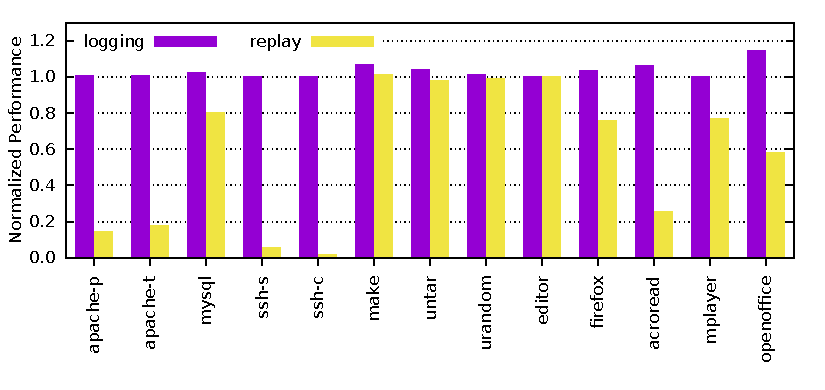
\includegraphics[width=2.3in]{figures/scribe/overhead}
    \vskip -0.21in
    % \captionsetup{justification=centering}
    \smallcaption{Recording runtime overhead}
    \vskip 0.3in
    \label{scribe:fig:overhead}
  \end{minipage}
  \begin{minipage}[b]{0.33\linewidth}
    \centering
    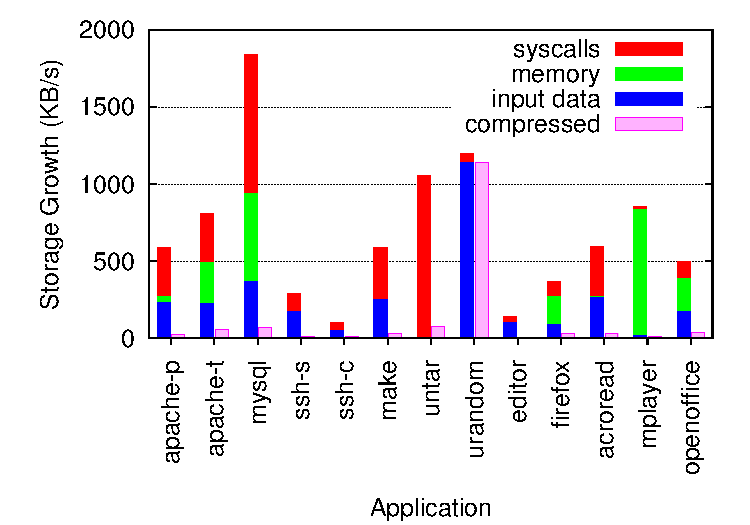
\includegraphics[width=2.3in]{figures/scribe/storage}
    \vskip -0.21in
    % \captionsetup{justification=centering}
    \smallcaption{Recording storage growth}
    \vskip 0.3in
    \label{scribe:fig:storage}
  \end{minipage}
  \begin{minipage}[b]{0.33\linewidth}
    \centering
    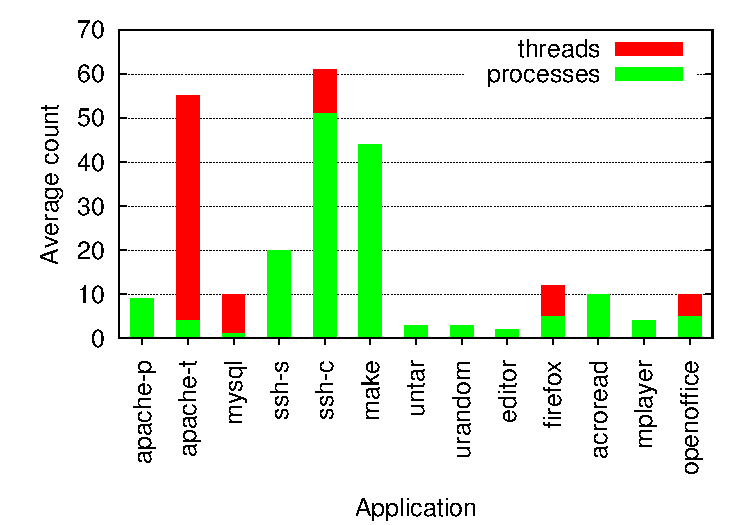
\includegraphics[width=2.3in]{figures/scribe/totals}
    \vskip -0.21in
    % \captionsetup{justification=centering}
    \smallcaption{No. of processes and threads}
    \vskip 0.3in
    \label{scribe:fig:totals}
  \end{minipage}
  \vskip -0.35in
  \end{figure*}
  \begin{figure*}
  \begin{minipage}[b]{0.33\linewidth}
    \centering
    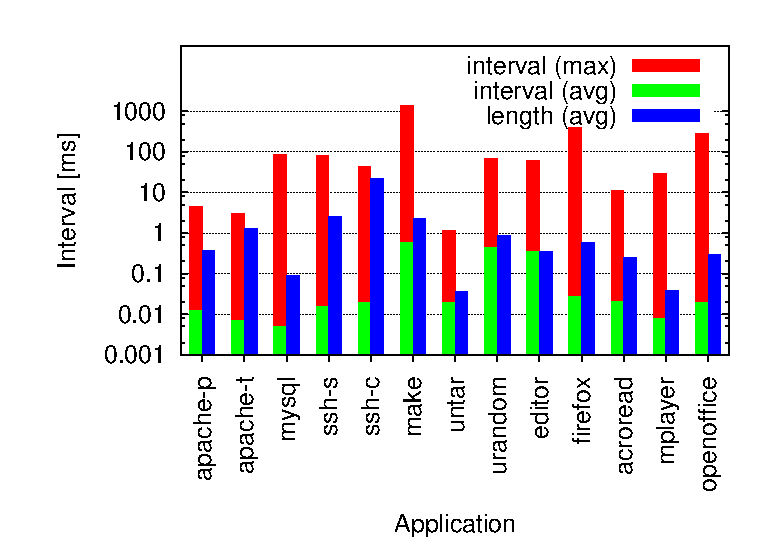
\includegraphics[width=2.3in]{figures/scribe/syncpts2}
    \vskip -0.21in
    % \captionsetup{justification=centering}
    \smallcaption{Sync points interval and length}
    \vskip 0.2in
    \label{scribe:fig:syncpts}
  \end{minipage}
  \begin{minipage}[b]{0.33\linewidth}
    \centering
    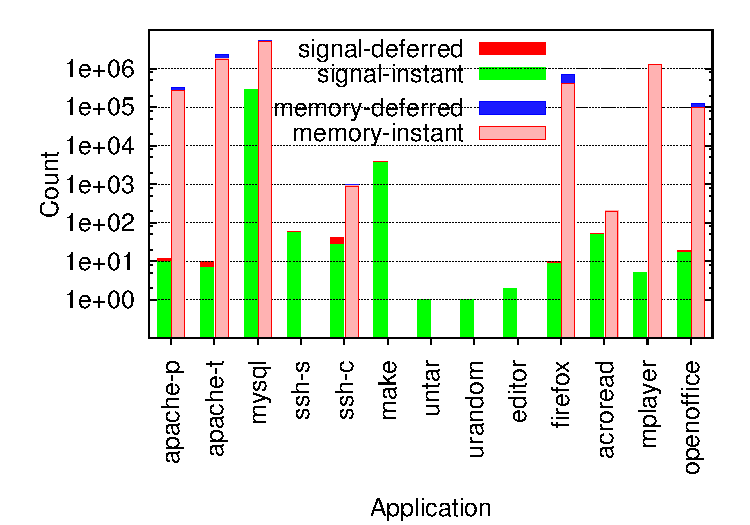
\includegraphics[width=2.3in]{figures/scribe/stats}
    \vskip -0.21in
    % \captionsetup{justification=centering}
    \smallcaption{Count of signals and memory}
    \vskip 0.2in
    \label{scribe:fig:stats}
  \end{minipage}
  \begin{minipage}[b]{0.33\linewidth}
    \centering
    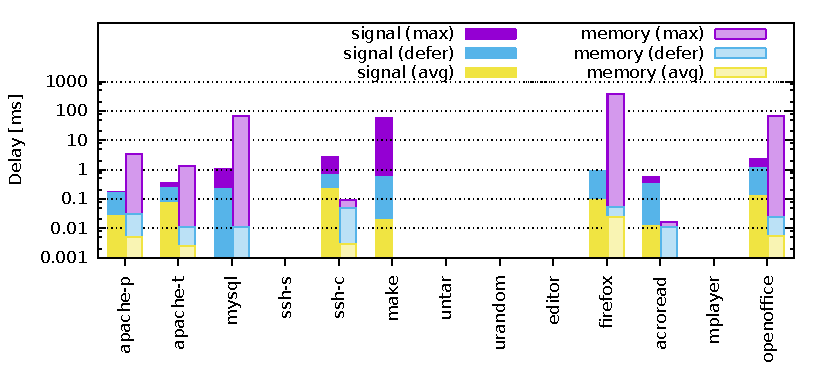
\includegraphics[width=2.3in]{figures/scribe/delays2}
    \vskip -0.21in
    % \captionsetup{justification=centering}
    \smallcaption{Delay of signals and memory}
    \vskip 0.2in
    \label{scribe:fig:delays}
  \end{minipage}
  \vskip -0.3in
\end{figure*}

We measured the performance of \scribe{} using the benchmark workloads
listed in Table~\ref{scribe:tab:scenarios}.  Applications were all run with
their default configurations.  Workloads were selected to
stress the system to provide a conservative measure of performance.
For example, {\tt firefox} runs the widely used SunSpider benchmark
designed to measure real-world web browser JavaScript performance.  
We also included benchmarks that emulate multiple interactive users
such as {\tt ssh-s} and {\tt ssh-c}, which open multiple concurrent
SSH sessions, each having an emulated user input text into a vi editor
at world-record typing speed~\cite{typist} to create a 5 KB file, then
exiting. We focus on quantifying the performance overhead and storage
requirements of running applications with \scribe{} in terms of the
cost of continuously recording the execution, and speedup of replayed
execution versus recorded execution. Previous work shows that the
overhead of the virtual execution environment is
small~\cite{zap-systor10,zap02}.

Figure~\ref{scribe:fig:overhead} shows the performance overhead of recording
the application workloads.  Performance is measured as completion time
in all cases except for {\tt apache-p} and {\tt apache-t} which report
performance in completed requests per second. No frames were dropped
during logging of {\tt mplayer} playback.  Results are shown
normalized to native execution without recording.  Recording overhead
was under 2.5\% for server applications and under 7\% for all desktop
applications except for {\tt openoffice}, which was 15\%.  For all desktop
applications, there was no user noticeable degradation in interactive
performance.

Figure~\ref{scribe:fig:overhead} also shows the performance of replaying the
applications workloads. Performance is measured as completion time,
normalized to execution with recording. Replaying speedup relative to
recording was at least 1 in all cases, and reached as much as a factor
of 70 for {\tt ssh-c}. The results demonstrate that \scribe{} can
replay applications at least as fast as it records, as expected. This
is useful for fault-tolerant systems to guarantee that replay on the
backup does not slow down execution on the primary.

Two factors contribute to replay speedup: omitted in-kernel work due
to system calls partially or entirely skipped (e.g. network output),
and compressed time due to time waiting skipped at replay (e.g. timer
expiration). Application that do neither perform the same work whether
recording or replaying, and sustain speedups close to 1. This includes
computation-intensive workloads such as {\tt make}, {\tt urandom},
{\tt untar}, and {\tt editor}. The speedup increases as the workload
exhibits more idle time in sleeping or blocking (mostly waiting for
input events). For instance, {\tt mplayer} spends about 23\% of the
time sleeping during recording, and its replay speedup is roughly
1.3. Replay speedup is noticeably larger for workloads
that spend much of their time sleeping: 3.9 for {\tt acrobat},
7.1 for {\tt apache-p}, and 5.8 for {\tt apache-t}.
Interactive workloads obtained
the largest speedups: 19 for {\tt ssh-s} and 70 for {\tt ssh-c}.

Figure~\ref{scribe:fig:storage} shows the storage growth rate of recording.
Storage requirements are decomposed into memory-related events ({\tt
  memory}), nondeterministic input data returned by system calls ({\tt
  input data}), and other data which is primarily system call return
values and rendezvous points ({\tt syscalls}).  The storage growth
rates ranged from 100\KB{}/\secs{} for {\tt ssh-c} to almost
1.9\MB{}/\secs{} for {\tt mysql}.  These storage requirements are
quite modest.  When compressed using lzma, storage growth rates
dropped to between 1 to 90\KB{}/\secs{} for all scenarios except {\tt
  urandom}, whose storage growth rate 
remained a bit over 1.1\MB{}/\secs{}.  Most of the log of
{\tt urandom} is due to input of random data, which does not compress
well.  

Figure~\ref{scribe:fig:totals} shows the average number of processes and
threads running for each application scenario.  The sum of the two is
the average number of total Linux tasks running.  All workloads except {\tt
  editor} consisted of multiple processes or threads, demonstrating
\scribe{}'s ability to record and replay real multi-process and
multi-threaded application workloads.  Five of the scenarios used
threads: {\tt apache-t}, {\tt mysql}, {\tt ssh-c}, {\tt firefox}, and 
{\tt openoffice}. For all of these scenarios except {\tt ssh-c}, this
correlates with the majority of the log storage consisting of memory
events, as shown in Figure~\ref{scribe:fig:storage}.  The threads in {\tt
  ssh-c} are
used in the benchmark to manage
concurrent sessions.  They involve very little contention over shared
memory, and therefore do not contribute much to the log size.
Conversely, {\tt apache-p} shows mild shared memory activity despite
being a multi-process application rather than multi-threaded. 

Figure~\ref{scribe:fig:syncpts} shows the time interval between consecutive
per process sync points for each application scenario. The average
time interval is measured per process then averaged over all
processes.  It is at most 30\us{} for all scenarios except {\tt make},
{\tt urandom} and {\tt editor}, for which it is less than 500\us{}.
These three are CPU intensive workloads that produce sync points only
due to system calls.
The maximum time interval between sync points for almost all
application workloads was less than 100\ms{}, which is also not large
and similar to the scheduling time quantum in Linux.  The maximum time
interval for three application workloads, {\tt make}, {\tt firefox},
and {\tt openoffice}, was higher, but only occurred once,
during the startup of each application.  If we exclude these outliers
and compute the 99th percentile of the time interval between sync
points, the time interval is less than 10\ms{}.

Figure~\ref{scribe:fig:syncpts} also shows the average length of sync points
per process for each application scenario. It is at least 300\us{} for
all scenarios except {\tt untar} and {\tt mplayer}, in which it is
over 50\us{}. More importantly, in all workloads the average time
spent at a sync point is significantly larger---over an order of
magnitude in most cases---than the time spent between sync point, or
outside sync points. Processes persist longer at sync points whenever,
for example, they block on I/O in a system call or wait for page
ownership transfer. During the time intervals within sync points,
asynchronous events for a process are delivered instantly and need not
be deferred. In other words, on average, most of the time asynchronous
events can be delivered promptly; and if not, then they are delayed
for a short period.  This establishes the empirical grounds for
\scribe{}'s reliance on sync points to successfully convert
asynchronous events to synchronous ones in a timely manner.

Figure~\ref{scribe:fig:stats} shows the total number of signals and shared
memory page faults due to \scribe{}'s page ownership management mechanism
for each application scenario.  Page faults not due to \scribe{} are
not included.  The totals are decomposed into those that are handled
instantly versus those that need to be deferred until a sync point is
reached.  The measurements show that \scribe{} provides
low-overhead execution recording even in the presence of a large
number of asynchronous events.  
Nearly all asynchronous events of
either type are handled instantly as they arrive, because the process
that is the target of these events is already executing in the
kernel at a sync point.  Sync points not only happen frequently
enough, but also endure long enough, that the vast majority of
asynchronous events can be handled immediately without being deferred.

Observe in Figure~\ref{scribe:fig:stats} that asynchronous events due to
shared memory page faults predominate over signals in scenarios that
involve multiple threads or shared memory. In these scenarios, page
faults due to \scribe{}'s page ownership management occur in larger
numbers, and, since they themselves are sync points, they contribute
to the pool of available sync points. The fraction of sync points due
to shared memory page faults of the total number of sync points ranges
from 10\% in {\tt apache-p}, to 30\% in {\tt mysql}, {\tt apache-t},
{\tt firefox}, and {\tt openoffice}, and up to 50\% in {\tt mplayer}.
In other words, applications that need sync points for shared memory
accesses are also likely to have sync points more frequently.

Figure~\ref{scribe:fig:delays} shows the amount of delay incurred for signals
and shared memory accesses. Signals were delayed at most 100\us{}
on average, except {\tt ssh-c}, which reached 220\us{}. The average
delay for only those few deferred signals that could not be handled
instantly was at most 1\ms{}. CPU intensive workloads without shared
memory produce sync points only due to system calls, and sustain longer
delays for deferred signals.  For example, in {\tt make}, 135 SIGCHLD
signals were deferred as the parent process waited to be scheduled
while compilations occupied the CPUs. Only when it was scheduled, it
reached a sync point and handled the signal. However, even without
\scribe{}, when the signal is delivered instantly, the parent process
would only handle the signal after a comparable delay since it would
still wait to be scheduled.  In multi-threaded workloads, the
delays for signals are longer, despite the addition of sync points due
to shared memory accesses. This is because our prototype only
considered sync points due to system calls for deferred signals. The
delays would probably be more comparable to those for shared memory
access if sync points due to shared memory were also used.

Unlike with signals, when a shared memory event occurs, the process
that faulted blocks until access is granted. Thus, whether memory
events are delayed and for how long is pivotal for the performance of
the system. Fortunately, shared memory accesses introduce numerous
additional sync points due to page ownership transfers. The average
delay for shared memory accesses was less than 25\us{}. If we consider
only deferred shared memory accesses that could not be handled
instantly, the average delay increases modestly to at most 60\us{}.
These delays are comparable to the native service time of a page
fault. \scribe{}'s sync points convert page ownership transfers from
asynchronous events to synchronous events with negligible impact on
page fault performance, since most asynchronous events are handled
instantaneously.

Finally, through all the executions of the application scenarios,
we have never observed a situation in which a process failed to reach a sync
point in a reasonable time, or at all.  Although \scribe{} has a 
mechanism in place to deal with delays that become too large, we did
not witness a need for this functionality in practice.  
Our experiences and results demonstrate that sync points occur
frequently and are useful for enabling deterministic replay.

\subsection{Related Work}
\label{scribe:sec:related}

Replaying program execution has been of interest for over 40
years~\cite{exdams}.  Hardware
mechanisms~\cite{hwrr,dmp,rerun,delorean,capo,strata,bugnet,fdr}
face a high implementation barrier and do not support record-replay on
commodity hardware.  Virtual machine
mechanisms~\cite{bressoud,revirt,smp-revirt,vmware}
require replaying operating system execution just to replay
application execution.  Almost none of them support replaying
multiprocessor virtual machines, and the ones that do incur an order
of magnitude worse overhead for common applications like
compilation due to kernel-level sharing, such as writing files to the
same directory~\cite{smp-revirt}.  Application and 
library mechanisms~\cite{liblog,r2,kendo,jockey} cannot provide
transparent record-replay for unmodified applications.  Programming
language mechanisms~\cite{dejavu,instant-replay,replay-pldi} do not
support widely-used applications written in languages that do not
provide record-replay primitives.  Unlike these approaches, \scribe{}
is an operating system mechanism.  It works at a higher-level
abstraction than hardware or virtual machine approaches to reduce
recording overhead.  It works at a lower-level abstraction than
application, library, and programming language approaches to provide
transparent record-replay for unmodified applications.

Other operating system mechanisms have also been
proposed~\cite{rr,bressoud-tft,flashback,rr-realtime} that interpose
between applications and the operating system.  None of them
provides record-replay for multi-threaded and
multi-process applications.  In fact, only TFT~\cite{bressoud-tft}
shows any record-replay results for real applications, namely 
{\tt gzip}, a single process application, but overhead was
quite high.  Unlike \scribe{}, TFT is only designed to replay a single
process.  Debugging using deterministic replay (DUDR)~\cite{rr-realtime}
presents only a paper design with no implementation or evaluation,
while Flashback~\cite{flashback} and RR~\cite{rr} are largely
incomplete with no results beyond those for a single, simple test
program.  In contrast, \scribe{} demonstrates for the first time that
record-replay of real multi-threaded and multi-process applications is
possible using an operating system approach.  

A key issue for operating system mechanisms is replaying the in-kernel
side effects of system calls.  This must be done for at least some
system calls in all replay systems.  

Previous approaches
do not solve the important problem of nondeterminism arising from
the order of execution of related system calls.  TFT only replays a
single process, so this issue does not arise.  DUDR and Flashback
hypothesize counting instructions to know when context switches occur
to track exact scheduling order to know the order of system call
execution among processes.  However, they provide no mechanism for
obtaining and using the required cycle accurate counters, and the
approach itself does not work for multiprocessors.  RR suggests
instrumenting the system call interface, but provides no actual
mechanism to do it.  In contrast, \scribe{} provides a new mechanism
using rendezvous points that solves this problem without tracking
exact scheduling order.  \scribe{}'s mechanism does not require
hardware support and works for multiprocessor systems. 

Record-replay systems must record the exact location in an instruction
stream at which an asynchronous event occurs.
This can be done by adding hardware support, modifying
applications, or writing applications with new language primitives to
record exactly when the application receives the event.
To do this on commodity hardware without application changes, all
previous approaches that deal with this
issue~\cite{bressoud,revirt,smp-revirt,slye96}
rely on the existence of a cycle accurate instruction counter.
To deal with interrupt lag~\cite{hwcount-isas06}, replay is done by
interrupting execution some time before the asynchronous event should
occur, 
setting a breakpoint on the instruction at which it should
occur, then stopping at every breakpoint to see if the instruction
counter matches the recorded value.  When they match, the asynchronous
event is delivered.
In contrast, \scribe{} introduces a fundamentally
different mechanism based on sync points that does not rely on
hardware performance counters.

TFT~\cite{bressoud-tft} proposed recording in periodic epochs for
fault tolerance, and then deferring the delivery of signals 
sent in each epoch until the respective epoch ends.  Epochs are
created by instrumenting applications to use counters to periodically
return control to TFT.  This also makes it easier to determine when
signals are delivered since they are delivered at well-defined epoch
boundaries.  The idea is similar to \scribe{}'s notion of deferring
signal delivery until sync points.  But, unlike TFT, \scribe{}
does not require instrumenting applications and does not define sync
points based on any measure of time or instruction counts.  Instead,
sync points are based on system calls, page faults, and traps that
occur as part of normal application execution.  Unlike TFT which only
supports replaying a single process, \scribe{} uses sync points to
enable replay of multi-process and multi-threaded applications on
multiprocessors. 

Besides \scribe{}, only SMP-ReVirt~\cite{smp-revirt} can transparently
replay multiprocessor workloads that use shared memory.
SMP-ReVirt replays multiprocessor virtual machines where multiple CPUs
may access shared memory.  It uses standard page protection to detect
memory races, and the concurrent read, exclusive write (CREW)
protocol~\cite{crew,instant-replay}.  To record exactly when page
access permissions switch from one CPU to another, SMP-ReVirt records
counter values in the same manner as it does for handling other
asynchronous events.  RR~\cite{rr} proposes a mechanism similar to
SMP-ReVirt, but notes problems with inaccuracy of hardware counters on
modern CPUs and has no record-replay results for any applications.
In contrast, \scribe{} avoids counter inaccuracies and introduces sync
points based on the 
assumption that real
applications perform frequent system activities that involve the
kernel.  This assumption is the antithesis of SMP-ReVirt's virtual
machine approach which must also record kernel execution.
For example, SMP-ReVirt incurs an order of magnitude worse
overhead than \scribe{} for kernel compilation due to frequent system
activities that result in kernel-level sharing.  While SMP-ReVirt can
provide whole system replay, \scribe{} can provide much more efficient
application replay.   

\subsection{Conclusions and Future Work}
\label{scribe:sec:conclude}

\scribe{} is the first operating system mechanism to provide transparent,
deterministic execution record and replay of multi-threaded and
multi-process applications on commodity multiprocessors and operating
systems.  \scribe{} records and replays multiple processes by
accounting for nondeterministic interactions among
processes and their execution environment.  \scribe{} introduces {\em
rendezvous points} to ensure correct partial ordering of execution
based on system call dependencies, and {\em sync points} to convert
asynchronous interactions that can occur at arbitrary times into
synchronous events that are much easier to record and replay.  
\scribe{} can transition an application  to running live at any time,
and use checkpoints to record and replay from any point in
time.

We have implemented \scribe{} without changing, relinking, or
recompiling applications, libraries, or operating system kernels, and
without any specialized hardware support. It works on commodity Linux
operating systems, and commodity multi-core and multiprocessor
hardware.  Our evaluation shows for the first time that an operating
system mechanism can correctly and transparently record and replay
multi-process and multi-threaded applications on multiprocessors.  The
evaluation also provides strong empirical evidence that 
real server and desktop applications perform frequent
operating system activities which can serve as sync points.  \scribe{}
recording overhead is modest for server applications including Apache
and MySQL, and for desktop applications including Firefox, Acrobat,
OpenOffice, parallel kernel compilation, and movie playback. Future
work will explore the utility of sync points for record-replay of
large-scale parallel applications.

\clearpage
\chapter{\racepro: Detection of Process Races in Deployed Systems}
\label{ch:racepro}

\section{Introduction} \label{racepro:sec:intro}

After presenting \scribe, our transparent record-replay engine most suited for
application debugging by capturing and reproducing hard to find bugs, we explore
ways to reveal dormant bugs in applications, and catch them before they happen.
Specifically, we explore the effect of bugs due to harmful process races in
software, and how to detect them using record-replay mechanisms.

While thread races have drawn much attention from the research
community~\cite{cui:tern:osdi10,racerx:sosp03,racefuzzer:pldi08,wu:loom:osdi10,yu:racetrack:sosp},
little has been done for \emph{process races}, where multiple
processes access an operating system (OS) resource such as a file or
device without proper synchronization.  
Process races are much broader than time-of-check-to-time-of-use
(\toctou) races or signal races~\cite{signal-race}.  A typical \toctou
race is an atomicity violation where the permission check and the use
of a resource are not atomic, so that a malicious process may slip in.
A signal race is often triggered when an attacker delivers two signals
consecutively to a process to interrupt and reenter a non-reentrant
signal handler.  In contrast, a process race may be any form of race.
Some real examples include a shutdown script that unmounts a file system
before another process writes its data, \code{ps | grep X} shows $N$
or $N+1$ lines depending on the timing of the two commands, and
\code{make -j} failures.

To better understand process races, we present the first study of real
process races.  We study hundreds of real applications across six
Linux distributions and show that process races are numerous and a real
threat to reliability and security.  For example, a simple search on
Ubuntu's software management site~\cite{launchpad} returns hundreds of 
process races.  Compared to thread races that typically corrupt volatile
application memory, process races are arguably more dangerous
because they often corrupt persistent and system resources.
Our study also reveals that some of their characteristics hint towards
potential detection methods.   

We then present \racepro, the first system for automatically detecting
process races beyond \toctou and signal races.  
\racepro faces three key challenges.  The first is scope:
process races are extremely heterogeneous.  They may involve many
different programs.  These programs may be written in different 
programming languages, run within different processes or threads,
and access diverse resources.  Existing detectors for thread or \toctou
races are unlikely to work well with this heterogeneity.

The second challenge is coverage: although process races are numerous,
each particular process race tends to be highly elusive.
They are timing-dependent, and tend to surface only in rare
executions.  Arguably worse than thread races, they may occur only under
specific software, hardware, and user configurations at specific
sites.  It is hopeless to rely on a few software vendors and beta
testing sites to create all possible configurations and executions for
checking. 

The third challenge is algorithmic: what race detection algorithm can
be used for detecting process races?  Existing algorithms assume
well-defined load and store instructions and thread synchronization
primitives.   However, the effects of system calls are often
under-specified and process synchronization primitives are very
different from those used in shared memory. For instance, what shared objects
does \code{execve} access?  In addition to reading the inode of the
executed binary, an obvious yet incomplete answer, \code{execve} also
conceptually writes to \code{/proc}, which is the root cause of the
\code{ps | grep X} race (\S\ref{racepro:sec:detect}).  Similarly, a
thread-join returns only when the thread being waited for exits, but
\code{wait} may return when any child process exits or any signal arrives.
Besides fork-wait, processes can also synchronize using
pipes, signals, \code{ptrace}, etc.
Missing the (nuanced) semantics of these system calls can lead to false positives
where races that do not exist are mistakenly identified and, even
worse, false negatives where harmful races are not detected. 

\racepro addresses these challenges with four ideas.  First, it checks
deployed systems \emph{in vivo}.  While a deployed system is running, \racepro
records the execution without doing any checking.  \racepro then
systematically checks this recorded execution for races \emph{offline},
when the deployed system is idle or by replicating the execution to a
dedicated checking machine.  By checking deployed systems, \racepro mitigates
the coverage challenge because all user machines together can create a
much larger and more diverse set of configurations and executions for
checking.  Alternatively, if a configuration or execution never occurs, it
is probably not worth checking.  By decoupling recording and
checking~\cite{decouple:usenix08}, \racepro reduces its performance overhead
on the deployed systems.

Second, \racepro records a deployed system as a system-wide, deterministic
execution of multiple processes and threads. \racepro uses lightweight OS
mechanisms developed in our previous work \scribe
to transparently and efficiently record nondeterministic interactions
such as related system calls, signals, and shared memory accesses.
No source code or modifications of
the checked applications are required, mitigating the scope challenge.
Moreover, since processes access shared OS resources through system
calls, this information is recorded at the OS level so that \racepro can
use it to detect races regardless of higher level program semantics.  

Third, to detect process races in a recorded execution,
\racepro models each system call by what we call
\emph{load and store micro-operations} to shared kernel objects. 
Because these two operations are well-understood by existing race
detection algorithms, \racepro can leverage these
algorithms, mitigating the algorithmic challenge.  To reduce manual
annotation overhead, \racepro automatically infers
the micro-operations a system call does by tracking how it
accesses shared kernel objects, such as inodes.  
Given these micro-operations, \racepro detects \emph{load-store
races} when two concurrent system calls access a common kernel object
and at least one system call stores to the object.
In addition, it detects \emph{wait-wakeup races} such as
when two child processes terminate simultaneously 
so that either may wake up a waiting parent.
To our knowledge, no previous algorithm directly handles wait-wakeup races.

Fourth, to reduce false positives and negatives, \racepro uses 
\emph{replay and go-live} to validate detected races, a core feature of \scribe.
A race detected based on the micro-operations may be either \emph{benign}
or \emph{harmful}, depending on whether it leads to a \emph{failure}, such
as a segmentation fault or a program abort.
\racepro considers a change in the order of the system
calls involved in a race to be an \emph{execution branch}.  To check
whether this branch leads 
to a failure, \racepro replays the recorded execution until the \emph{reordered}
system calls then resumes live execution.  It then runs a set of built-in or
user-provided checkers on the live execution to detect failures,
and emits a bug report only when a real failure is detected.
By checking many execution branches,
\racepro reduces false negatives.  By reporting only harmful races, it
reduces false positives. 

We have implemented \racepro in Linux as a set of kernel components for
record, replay, and go-live, and a user-space exploration engine for
systematically checking execution branches.  Our experimental results
show that \racepro can be used in production environments with only
modest recording overhead, less than 2.5\% for server and 15\% for
desktop applications.  Furthermore, we show that \racepro can detect
\nracepro real bugs due to process races in widespread Linux
distributions. 

This chapter is organized as follows.  \S\ref{racepro:sec:study} presents a
study of process races and several process race examples.
\S\ref{racepro:sec:overview} presents an overview of the \racepro architecture.
\S\ref{racepro:sec:record} describes the execution recording mechanism.
\S\ref{racepro:sec:detect} describes  the system call modeling using
micro-operations and the race detection algorithm.
\S\ref{racepro:sec:validate} describes how replay and go-live are used to
determine harmful races.  \S\ref{racepro:sec:eval} presents experimental
results. \S\ref{racepro:sec:related} discusses related work.
Finally, \S\ref{racepro:sec:conclusion} presents a summary and concluding remarks of this chapter.

\begin{table}[t]
\centering
\begin{tabular}{c|cc|ccc}
  \toprule
                                    & \multicolumn{2}{c|}{\bf Pages} & \multicolumn{3}{c}{\bf Bugs} \\
  {\bf Distribution} & {\bf Returned} & {\bf Sampled} & {\bf Total} & {\bf Process} & {\bf Thread} \\ \midrule
  Ubuntu              & 3330 & 300  & 45  & 42 (1)   & 3   \\
  Fedora/RedHat\,\,\, & 1070 & 100  & 52  & 30 (10)  & 22  \\
  Gentoo              & 2360 & 60   & 31  & 23 (10)  & 8   \\
  Debian              & 768  & 40   & 17  & 12 (4)   & 5   \\
  CentOS              & 1500 & 40   & 5   & 2 (0)    & 3   \\
  \midrule
  {\bf Total}         & 9028 & 540  & 150 & 109 (25) & 41  \\
  \bottomrule
\end{tabular}
\caption{{\bf Summary of Collected Pages and Bugs.}}
\label{racepro:tab:data}
\end{table}


\section{Process Race Study} \label{racepro:sec:study}

We conducted a study of real process races with two key questions in
mind.  First, are process races a real problem?  Second, what are their
characteristics that may hint towards how to detect them?  We
collected bugs from six widespread Linux distributions, namely 
Ubuntu, RedHat, Fedora, Gentoo, Debian, and CentOS.  For each
distribution, we launched a search query of ``race'' on the distribution's
software management website.  We manually examined a random sample of
the returned pages, identified all unique bugs in the sampled pages,
and classified these bugs based on whether they resulted in process
or thread races.  Raw data of the studied bugs is 
available~\cite{all-resource-races}.
\S\ref{racepro:sec:findings} presents our findings. \S\ref{racepro:sec:example}
describes four process race examples from the most serious to the
least. 

\subsection{Findings} \label{racepro:sec:findings}

Table~\ref{racepro:tab:data} summarizes the collected pages and bugs;
Fedora and Redhat results are combined as they share the same
management website.   For each distribution, we show the number of
pages returned for our query (Returned), the number of pages sampled
and manually examined (Sampled), the number of process races
(Process) and the subset of
which were \toctou races, the number of thread races
(Thread), and the total number of bugs in the sampled pages (Total).

\para{Process races are numerous.}  Of the \nbug sampled bugs, \nprace
resulted in process races, a dominating majority; the other \nmrace
bugs resulted in thread races.  However, thread races are
likely underrepresented because the websites we searched are heavily
used by Linux distribution maintainers, not developers of individual
applications.  Of the \nprace process races, 
\nnottoctou are not \toctou races and therefore cannot
be detected by existing \toctou detectors. 
Based on this sample, the 7,498 pages that our simple search returned
may extrapolate to over 1,500 process races.  Note that our
counting is very conservative: the sampled pages contain an additional
\npraceunconfirmed likely process races, but the pages did
not contain enough information for us to understand the cause, so we
did not include them in Table~\ref{racepro:tab:data}.

\begin{figure}[t]
  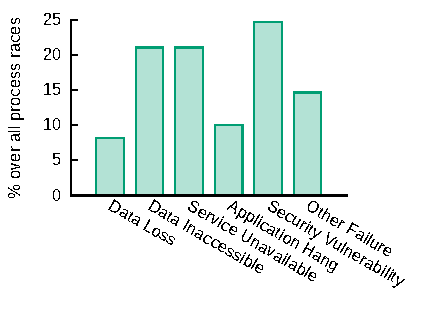
\includegraphics[width=0.54\linewidth,valign=t]{figures/racepro/race-effects2.pdf}
  \vspace{-2em}
  \hfill
  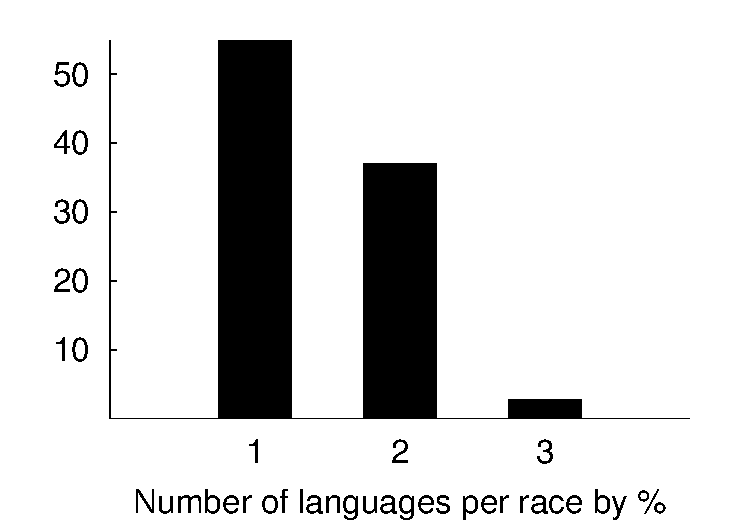
\includegraphics[width=.45\linewidth,valign=t]{figures/racepro/race-languages}
  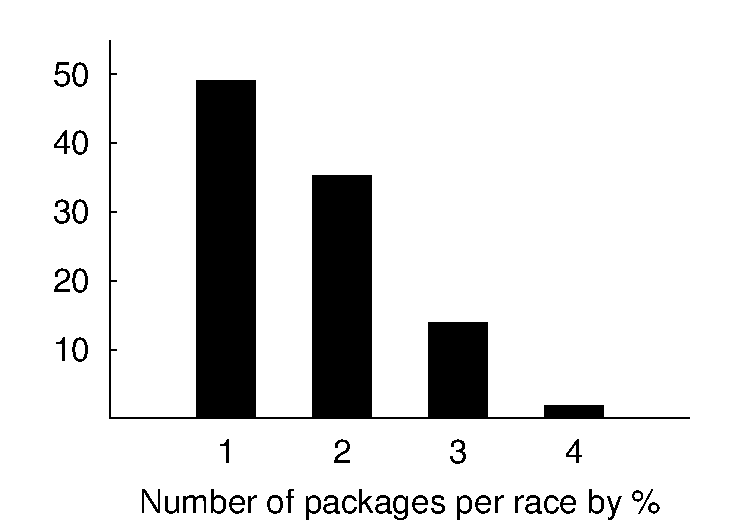
\includegraphics[width=.45\linewidth]{figures/racepro/race-packages}
  \hfill
  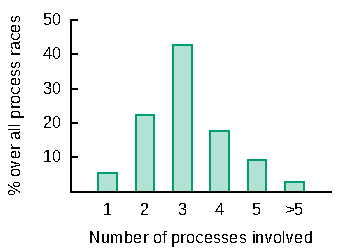
\includegraphics[width=.45\linewidth]{figures/racepro/race-processes}
\caption{{\bf Process Races Breakdown.}
  X axis shows the race effect, programming languages, the number of software packages, or processes involved.
  Y axis shows the percentage of process races that involve the specific effect, languages, packages, or processes.
  To avoid inflating the number of processes, we count a run of a shell script
  as one process.  (Each external command in a script causes a \code{fork}.)}
\label{racepro:fig:breakdown}
\end{figure}

\para{Process races are dangerous.}  Compared to thread races that
typically corrupt volatile application memory, process races
are arguably more dangerous because they often corrupt persistent and system resources.
Indeed, the sampled process races caused security breaches, files and databases to
become corrupted, programs to read garbage, and processes to get stuck
in infinite loops. The top right graph in Figure~\ref{racepro:fig:breakdown} summarizes the effects of
all process races from Table~\ref{racepro:tab:data}.

\para{Process races are heterogeneous.}  The sampled process races
spread across over 200 programs, ranging from server
applications such as MySQL, to desktop applications such as OpenOffice,
to shell scripts in Upstart~\cite{upstart}, an event-driven
replacement of System V \code{init} scripts.  Figure~\ref{racepro:fig:breakdown}
breaks down the process races by packages, processes, and
programming languages involved.  Over half of the \nprace process races,
including all examples described in \S\ref{racepro:sec:example}, require 
interactions of at least two programs.  These programs are written in
different programming languages such as C, Java, PHP, and shell scripts,
run in multiple processes, synchronize via \code{fork} and \code{wait},
pipes, sockets, and signals, and access resources such as files, devices,
process status, and mount points.

This heterogeneity makes it difficult to apply existing detection methods
for thread races or \toctou races to process races.  For instance, static thread
race detectors~\cite{racerx:sosp03} work only with one program
written in one language, and dynamic thread race
detectors~\cite{yu:racetrack:sosp} work only with one process.  To
handle this heterogeneity, \racepro's race detection should be
system-wide. 

\para{Process races are highly elusive.} Many of the process races,
including Bug 1 and 3 described in
\S\ref{racepro:sec:example}, occur only due to site-specific software,
hardware, and user configurations.  Moreover, many of the sampled
process races, including all of those described in
\S\ref{racepro:sec:example}, occur only due to rare runtime factors. For
example, Bug 1 only occurs when a database shutdown takes longer 
than usual, and Bug 2 only occurs when a signal is delivered right 
after a child process exited.
These bugs illustrate the advantage of checking deployed systems, so that
we can rely on real users to create the diverse configurations and
executions to check.

\para{Process race patterns.}  Classified by the causes, the
\nprace process races fall into two categories.  Over two
thirds (\norder) are execution order
violations~\cite{lu:concurrency-bugs}, 
such as Bug 1, 3, and 4 in \S\ref{racepro:sec:example},
where a set of events are
supposed to occur in a fixed order, but no synchronization operations
enforce the order.
Less than one third (\natomic) are atomicity violations, including all
\toctou bugs; most of them are the simplest load-store
races, such as Bug 2 in \S\ref{racepro:sec:example}. 
Few programs we studied use standard locks (\eg, \code{flock}) to
synchronize file system accesses among processes.
These patterns suggest that a lockset-based race detection algorithm is
unlikely to work well for detecting process races.  Moreover, it is crucial
to use an algorithm that can detect order violations.

\subsection{Process Race Examples} \label{racepro:sec:example}

\begin{figure}
\centering
\begin{minipage}{.4\textwidth}
  \begin{rbox}
\begin{lstlisting}[language=C,framexleftmargin=5pt]
child = fork()
setjmp(loc)
p = wait(...) [blocks...]
...          // child exits
p = wait(...) [...returns]
...          // signaled
longjmp(loc)
p = wait(...) // error (no child)
\end{lstlisting}
\end{rbox}
\vspace{-1.5em}
  \caption{{\bf dash-MySQL Race.}}
  \label{racepro:fig:dash-mysql}
\end{minipage}
\hspace{3em}
\begin{minipage}{.4\textwidth}
  \begin{rbox}
\begin{lstlisting}[language=C,framexleftmargin=5pt]
fd = open(H,RDONLY);
read(fd, buf, ...);
close(fd);
... // update buf
... // do work
fd = open(H,WRONLY|TRUNC);
write(fd, buf, ...);
close(fd);
\end{lstlisting}
\end{rbox}
\vspace{-1.5em}
      \caption{{\bf bash Race.}}
      \label{racepro:fig:bash}
\end{minipage}
\end{figure}

\para{Bug 1: Upstart-MySQL.}  \code{mysqld} does not cleanly terminate
during system shutdown, and the file system becomes corrupted.  This
failure is due to an execution order violation where \code{S20sendsigs},
the shutdown script that terminates processes, does not wait long
enough for MySQL to cleanly shutdown. The script then fails to unmount
the file system which is still in use, so it proceeds to reboot the
system without cleanly unmounting the file system.  Its occurrence
requires a combination of many factors, including the mixed use of
Systems V initialization scripts and Upstart, a misconfiguration so
that \code{S20sendsigs} does not wait for daemons started by Upstart,
insufficient dependencies specified in MySQL's Upstart configuration
file, and a large MySQL database that takes a long time to shut down.

\para{Bug 2: dash-MySQL.} The shell wrapper
\code{mysql\_safe} of the MySQL server daemon \code{mysqld} goes into an
infinite loop with 100\% CPU usage after a MySQL update.
This failure is due to an atomicity violation in \code{dash},
a small shell Debian uses to run daemons~\cite{dash}.  It occurs
when \code{dash} is interrupted by a signal unexpectedly.
Figure~\ref{racepro:fig:dash-mysql} shows the event sequence causing this race.
To run a new background job, \code{dash} forks a child process and
adds it to the job list of \code{dash}.  It then calls \code{setjmp} to save an execution
context and waits for the child to exit.  After the child exits,
\code{wait} returns, and \code{dash} is supposed to remove the child from
the job list.  However, if a signal is delivered at this time, \code{dash}'s
signal handler will call \code{longjmp} to go back to the saved 
context, and the subsequent \code{wait} call will fail because the child's
exit status has been collected by the previous \code{wait} call.  
The job list is still not empty, so \code{dash} gets stuck waiting for the
nonexistent child to exit.  Although this bug is in \code{dash}, it is
triggered in practice by a combination of \code{dash}, the \code{mysql\_safe}
wrapper, and \code{mysqld}.

\para{Bug 3: Mutt-OpenOffice.}  OpenOffice displays
garbage when a user tries to open a Microsoft (MS) Word attachment in the
Mutt mail client.
This failure is due to an execution order violation
when \code{mutt} prematurely overwrites the contents of a file
before OpenOffice uses this file.  It involves a
combination of Mutt, OpenOffice, a user configuration entry
in Mutt, and the \code{openoffice} shell script wrapper.  The user
first configures Mutt to use the \code{openoffice} wrapper to open
MS Word attachments.  To show an attachment, \code{mutt} saves the
attachment to a temporary file, spawns the configured viewer in a new
process, and waits for the viewer process to exit.  The \code{openoffice}
wrapper spawns the actual OpenOffice binary and exits at once.
\code{mutt} mistakes this exit as the termination of the actual viewer, and
overwrites the temporary file holding the attachment with all zeros,
presumably for privacy reasons.

\para{Bug 4: bash.} The \code{bash} shell history is corrupted.
This failure is due to an atomicity violation
when multiple \code{bash} shells write concurrently
to \code{.bash\_history} without synchronization.
When \code{bash} appends to the history file, it correctly uses
\code{O\_APPEND}.  However, it also occasionally reads back the history
file and overwrites it, presumably to keep the history file under a
user-specified size.  Figure~\ref{racepro:fig:bash} shows this problematic
sequence of system calls.  \code{bash} also runs this sequence when it
exits.  When multiple \code{bash} processes exit at the same time, the
history file may be corrupted. 

\section{Architecture Overview} \label{racepro:sec:overview}


\begin{figure}[]
  \centering
  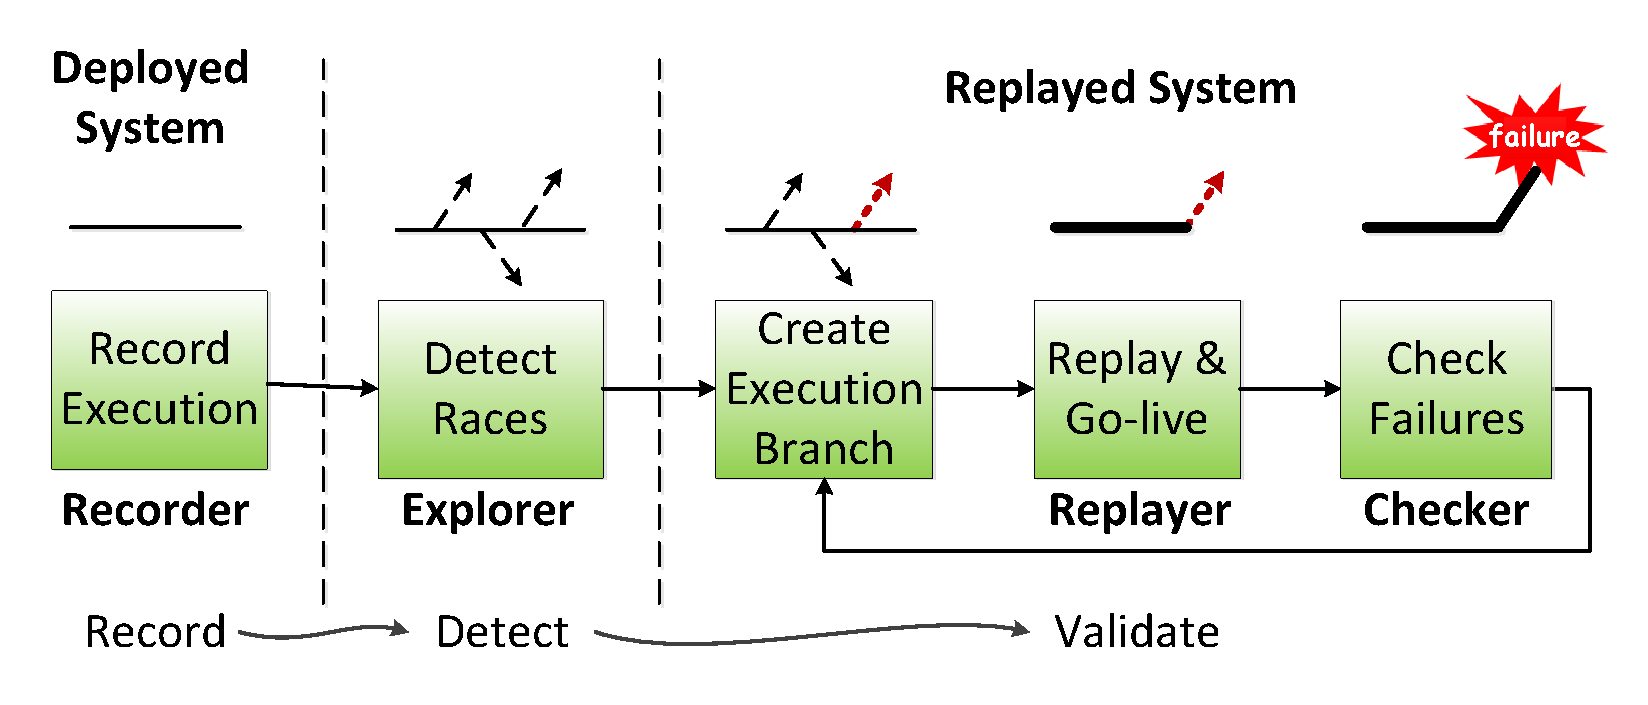
\includegraphics[width=0.9\linewidth]{figures/racepro/flow}
  \caption{{\bf \racepro Workflow.} Thin solid lines represent recorded
    executions; thick solid lines represent replayed executions.  Dashed
    arrows represent potentially buggy execution branches. The dotted
    thick arrow represents the branch \racepro selects to
    explore.} \label{racepro:fig:flow}
\end{figure}

\begin{figure}[]
  \centering
  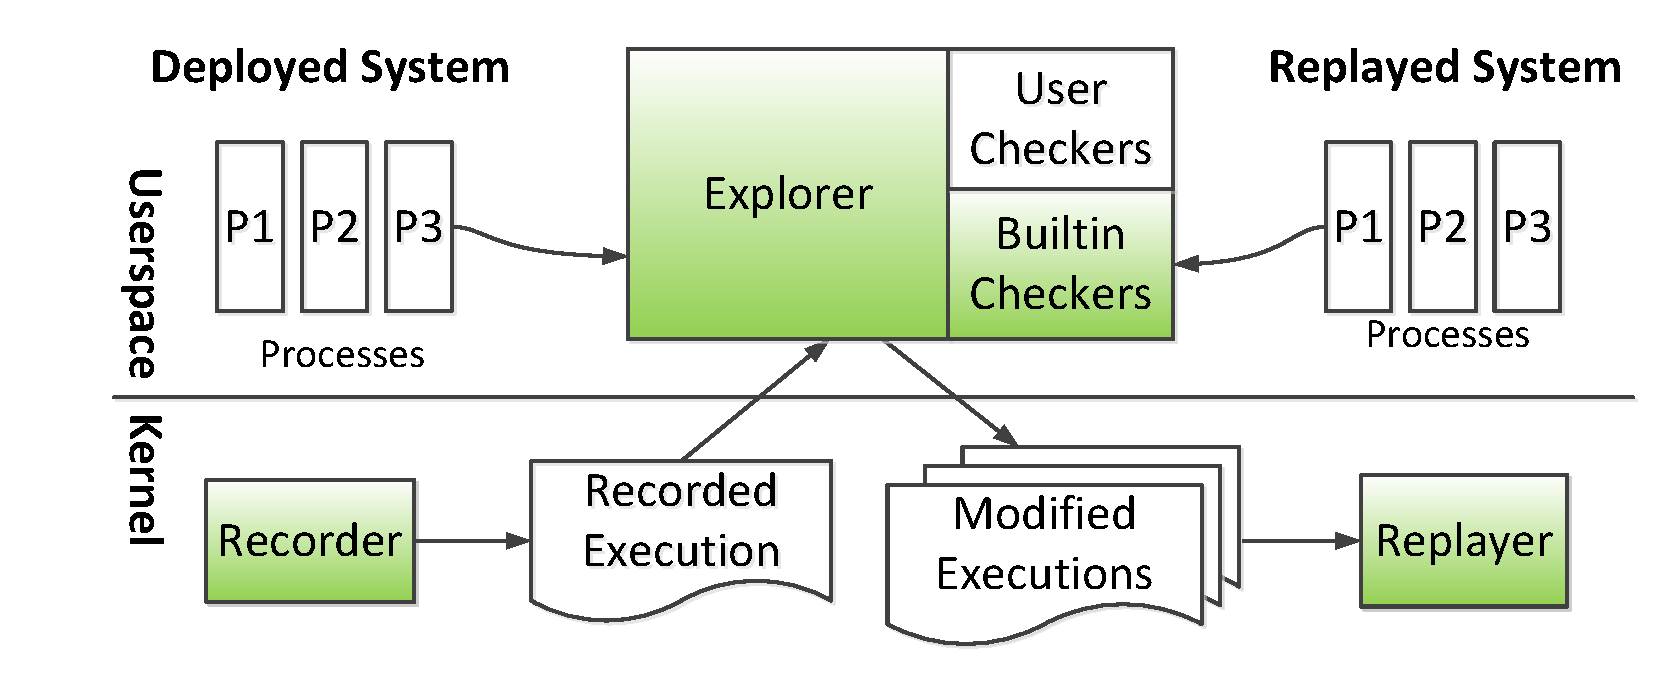
\includegraphics[width=0.9\linewidth]{figures/racepro/arch}
  \caption{{\bf \racepro Architecture.} Components are shaded. The recorder
    and the replayer run in kernel-space, and the explorer and the
    checkers run in user-space.  Recorded executions and modified
    executions are stored in files.} \label{racepro:fig:arch}
\end{figure}


\racepro is designed to automatically detect process races using the
workflow shown in Figure~\ref{racepro:fig:flow}.  
It consists of three steps,
the first of which runs on the deployed system, while the latter two can run
elsewhere on a separate replay system to avoid any performance
impact on the deployed system.
First, a \emph{recorder} records the execution of a deployed system
while the system is running and stores the recording in a log file.  Second,
an \emph{explorer} reads the log and detects load-store and wait-wakeup races
in the recorded execution.  Third, each race is validated to determine if
it is harmful.  An execution branch of the recorded execution
corresponding to each race is computed by systematically changing the
order of system calls involved in the race.  For each
execution branch, a modified log is constructed that is used to replay 
execution with the changed order of system calls.  A 
\emph{replayer} replays the respective modified log up to the
occurrence of the race, then causes it to resume live execution from
that point onward.  A set of built-in and user-provided \emph{checkers}
then check whether the execution results in misbehavior or a failure
such as a segmentation fault.  By examining the effects of a live
execution, we distinguish harmful races from false or benign ones,
thus reducing false
positives~\cite{pinsel:pldi07,racefuzzer:pldi08}. The live part 
of the re-execution is also recorded, so that users can
deterministically replay detected bugs for debugging.

Figure~\ref{racepro:fig:arch} shows the \racepro architecture used to support its
workflow.  Of the four main architectural components, the recorder
and the replayer run in kernel-space, and the explorer and checkers
run in user-space.  We will describe how \racepro records executions
(\S\ref{racepro:sec:record}) and detects (\S\ref{racepro:sec:detect}) and validates
(\S\ref{racepro:sec:validate}) races using these components.  

\section{Recording Executions} \label{racepro:sec:record}

\racepro's record-replay functionality builds on our previous work on
lightweight OS-level deterministic replay on
multiprocessors~\cite{scribe:sigmetrics10}.  This approach provides four key
benefits for detecting process races.  First, \racepro's recorder can 
record the execution of multiple processes and threads with low overhead
on a deployed system so that the replayer can later deterministically
replay that execution.  This makes \racepro's \emph{in vivo} checking approach
possible by minimizing the performance impact of recording deployed
systems.  Second, \racepro's record-replay is application-transparent; it
does not require changing, relinking, or recompiling applications or
libraries. This enables \racepro to detect process races that are
extremely heterogeneous involving many different programs written in
different program languages.  Third, \racepro's recorder operates at the
OS level to log sufficiently fine-grained accesses to shared kernel
objects so that \racepro's explorer can detect races regardless of
high-level program semantics~(\S\ref{racepro:sec:detect}).  Finally, \racepro's
record-replay records executions such that it can later transition 
from controlled replay of the recording to live execution at any
point.  This enables \racepro to distinguish harmful races from benign
ones by allowing checkers to monitor an application for
failures~(\S\ref{racepro:sec:reexec}). 

To record the execution of multiprocess and multithreaded
applications, \racepro records all nondeterministic interactions between
applications and the OS and saves the recording as a log file.  We
highlight how key interactions involving system calls, signals, and
shared memory are handled.

\para{System calls.}  Unlike previous
work~\cite{r2:osdi,srinivasan:flashback} that records and replays a total
order of system calls, \racepro records and replays a partial order of system
calls for speed.  \racepro enforces no ordering constraints among system
calls during record-replay unless they access the same kernel object
and at least one of them modifies it, such as a \code{write} and a
\code{read} on the same file.  In that case, \racepro records the order in
the kernel in which the object is accessed by the system calls and
later replays the exact same order of accesses.  This is done by 
piggybacking on the synchronization code that the kernel already has
for serializing accesses to shared objects.  These tracked accesses
also help detect process races in a recorded execution
(\S\ref{racepro:sec:detect}). 

Table~\ref{racepro:tab:resources} lists the kernel objects tracked by \racepro.
Most of the entries correspond one-to-one to specific low-level kernel
resources, including inodes, files, file-tables, memory maps, and
process credentials. The global entry corresponds to system-wide
kernel objects, such as the hostname, file system mounts, system time,
and network interfaces. For each such system-wide resource there
is a unique global kernel object used to track accesses to that
resource. The last two entries in the table, pid and ppid, provide a
synchronization point to track dependencies on process states. For
example, the pid entry of a process is used to track instances where
the process is referenced by another process, \eg, through a system
call that references the process ID or through the \code{/proc} file
system. The ppid entry is used to track when an orphan process is
re-parented, which is visible through the \code{getppid} system call.
Both pid and ppid correspond to identifiers that are visible to
processes but cannot be modified explicitly by processes.

\begin{table}[t]
\centering
\begin{tabular}{ll}
  \toprule
{\bf Object} & {\bf Description} \\ \midrule
inode       & file, directory, socket, pipe, tty, pty, device \\
file        & file handle of an open file \\
file-table  & process file table \\
mmap        & process memory map \\
cred        & process credentials and capabilities, \eg, user ID \\
global      & system-wide properties (\eg, hostname, mounts) \\
pid         & process ID (access to process and \code{/proc}) \\
ppid        & parent process ID (synchronize \code{exit/getppid}) \\
  \bottomrule
\end{tabular}
\caption{{\bf Shared Kernel Objects Tracked.}} \label{racepro:tab:resources}
\end{table}

The recorder only tracks kernel objects whose state is visible
to user-space processes, either directly or indirectly.  For example,
inode state is accessible via the system call \code{lstat}, and
file-table state is visible through resolving of file descriptor in
many system calls. \racepro does not track accesses to kernel
objects which are entirely invisible to user-space.
This avoids tracking superfluous
accesses that may pollute the race detection results with unnecessary
dependencies.
For example, both the \code{fork} and \code{exit} system calls access the
kernel process table, but the order is unimportant to user-space. It
only matters that the lifespan of processes is observed correctly, 
which is already tracked and enforced via the pid resource.  If \racepro
tracked accesses to the kernel process table, it would mistakenly
conclude that every two \code{fork} system calls are ``racy'' because they
all modify a common resource~(\S\ref{racepro:sec:detect}).  One complication 
with this approach is that if the kernel object in question controls
assignment of identifiers (\eg, process ID in the \code{fork} example),
it may assign different identifiers during replay because the original
order of accesses is not enforced. To address this problem, \racepro
virtualizes identifiers such as process IDs to ensure the same values
are allocated during replay as in the recording.

\para{Signals.}
Deterministically replaying signals is hard since they must be
delivered at the exact same instruction in the target execution flow
as during recording.  To address this problem,
\racepro uses \emph{sync points} that correspond to synchronous kernel entries
such as system calls.  Sending 
a signal to a target process may occur at any time during the target
process's execution.  However, \racepro defers signal delivery until sync
points occur to make their timing deterministic so they are easier to
record and replay efficiently.  Unlike previous approaches, sync
points do not require hardware counters or application modifications,
and do not adversely impact application performance because they occur
frequently enough in real server and desktop applications due to OS
activities.  

\para{Shared memory.}
\racepro combines page ownership with sync points to
deterministically record and replay the order of shared memory
accesses among processes and threads.  Each shared memory page is
assigned an owner process or thread for some time interval.  The owner
can exclusively modify that page during the interval and treat it like 
private memory, avoiding the need to track all memory accesses during such
ownership periods.  Transitioning page ownership from one process or
thread to another is done using a concurrent read, exclusive write
(CREW) protocol~\cite{smp-revirt,instant-replay}.  To ensure
that ownership transitions occur at precisely the same location 
in the execution during both record and replay, \racepro defers such
transitions until the owner reaches a sync point.  When a process
tries to access an owned page, it triggers a page fault, notifies the owner,
and blocks until access is granted.  Conversely, each owner checks for
pending requests at every sync point and, if necessary, gives up 
ownership.   Page faults due to the memory interleaving under
the CREW protocol are synchronous kernel entries that
deterministically occur on replay and hence are also used as sync 
points. 

\section{Detecting Process Races} \label{racepro:sec:detect}

\racepro flags a set of system calls as a race if (1)~they are
\emph{concurrent} and therefore could have executed in a different
order than the order recorded, (2)~they access a common resource
such that reordering the accesses may change the outcome of the
execution.  To determine whether a set of system calls are concurrent, 
\racepro constructs a happens-before~\cite{lamportclock} graph for the
recorded execution (\S\ref{racepro:sec:graph}).  To determine whether a set of
system calls access common resources, \racepro obtains the shared kernel
resources accessed by system calls from the log file and models the
system calls as \emph{load} and \emph{store} micro-operations
(\S\ref{racepro:sec:model}) on those resources.  \racepro then runs a set of
happens-before based race detection algorithms to detect load-store
and wait-wakeup races (\S\ref{racepro:sec:potential}).

\subsection{The Happens-Before Graph} \label{racepro:sec:graph}

We define a partial ordering on the execution of system calls called
\emph{inherent} happens-before relations.  We say that system call
$S_1$ \emph{inherently} happens-before system call $S_2$ if (1)~$S_1$
accesses some resource before $S_2$ accesses that resource, (2)~there
is a dependency such that $S_2$ would not occur or complete unless
$S_1$ completes, and (3)~the dependency must be inferable from the
system call semantics.  For example, a \code{fork} that creates a child
process inherently happens-before any system call in the child
process, and a \code{write} to a pipe inherently happens-before 
a blocking \code{read} from the pipe.  On the other hand, there is no
inherent happens-before relation between a \code{read} and subsequent 
\code{write} to the same file.

\racepro constructs the happens-before graph using only inherent
happens-before relations, as they represent the basic constraints on
the ordering of system calls.  Given a recorded
execution, \racepro constructs a happens-before graph for all recorded
system call events by considering pairs of such events.  If two events
$S_1$ and $S_2$ occur in the same process and $S_2$ is the next
system call event that occurs after $S_1$, \racepro adds a directed edge
$S_1\rightarrow S_2$ in the happens-before graph.  If two events $S_1$
and $S_2$ occur in two different processes, \racepro adds a directed edge
$S_1\rightarrow S_2$ in four cases: 

\begin{itemize}
\item $S_1$ is a \code{fork} call, and $S_2$ is the corresponding
  \code{fork} return in the child process;
\item $S_1$ is the \code{exit} of a child process, and $S_2$ is the
  corresponding \code{wait} in the parent;
\item $S_1$ is a \code{kill} call, and $S_2$ is the corresponding signal
  delivery in the target process; or
\item $S_1$ is a stream (\eg, pipe or socket) write, and $S_2$ is a
  read from the same stream and the data written and the data read
  overlap.
\end{itemize}

We say that event $S_1$ \emph{happens-before} $S_2$ with respect to a
happens-before graph iff there is a directed path from $S_1$ to
$S_2$ in the happens-before graph.  Two events are \emph{concurrent}
with respect to a happens-before graph iff neither happens before
the other. 

\racepro also computes the vector-clocks~\cite{vectorclock} for all the
system calls in the happens-before graph.  By definition, the
vector-clock of $S_1$ is earlier than the vector-clock of $S_2$ iff
$S_1$ \emph{happens-before} $S_2$ with respect to the graph, so comparing
the vector-clocks of system calls is a fast and efficient way to test
whether they are concurrent.

Our definition of inherent happens-before does not capture all
dependencies that may constrain execution ordering. It may be missing
happens-before edges that depend on the behavior of the application
but cannot be directly inferred from the semantics of the system calls
involved. For example, the graph does not capture dependencies between
processes via shared memory. It also does not capture dependencies
caused by contents written to and read from files. For example, one
can implement a fork-join primitive using read and write operations on
a file.  In some cases, such inaccuracies may make \racepro more
conservative in flagging racy system calls and thereby identify
impossible races.  However, such cases will be filtered later by
\racepro's validation step (\S\ref{racepro:sec:validate}) and will not be reported.

\begin{figure}[]
\centering
\hspace*{-1.4em}
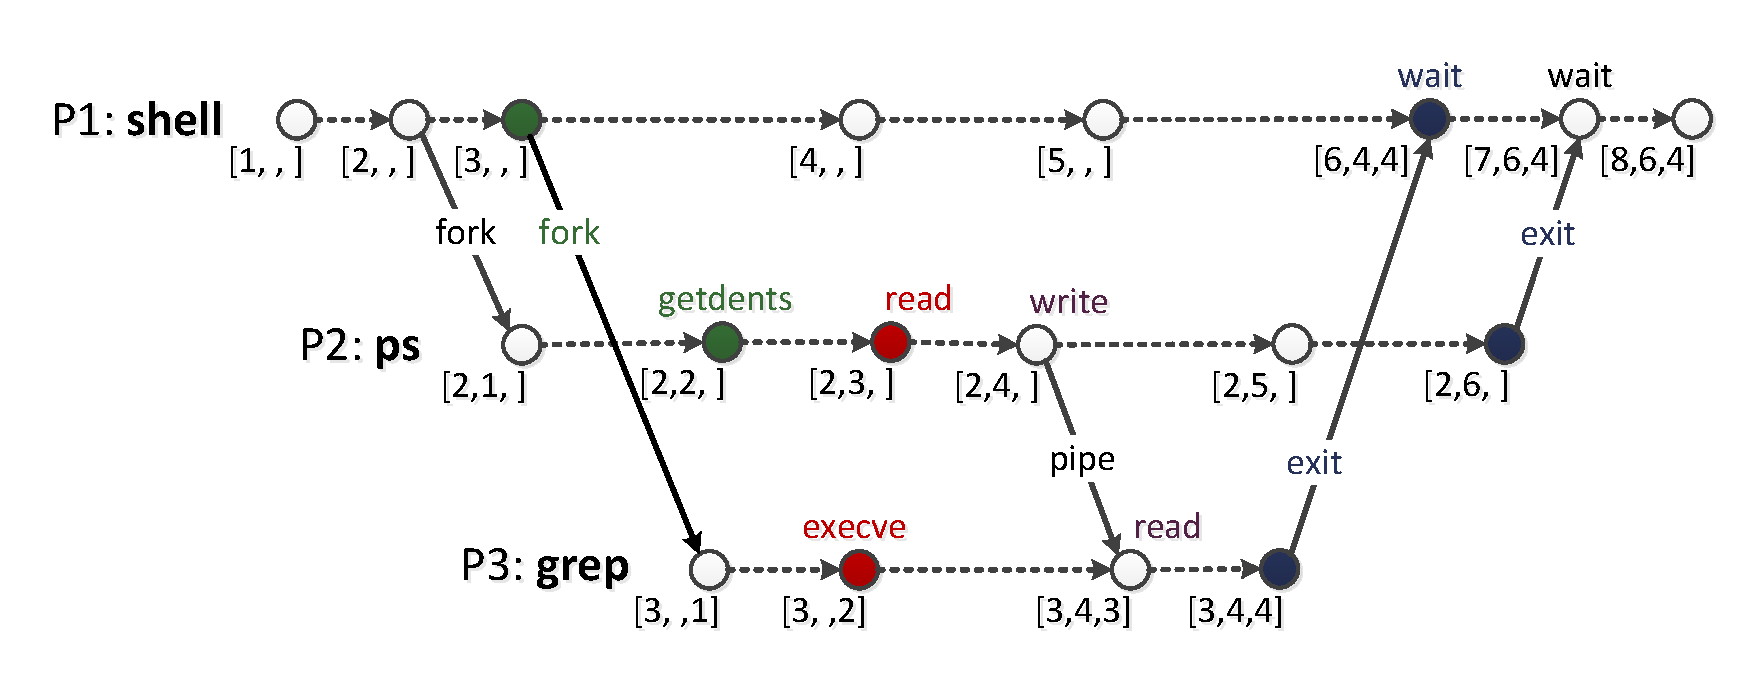
\includegraphics[width=1.05\linewidth]{figures/racepro/psgrep}
\caption{{\bf The Happens-Before Graph for \code{ps | grep X}.}
  $P_{i=1,2,3}$ represent the processes involved.
  $[i,j,k]$ represent vector-clocks.
  The \code{read} of process $P_2$ and the \code{execve} of
  $P_3$ form a load-store race~(\S\ref{racepro:sec:load-store}), and so do the
  second \code{fork} of $P_1$ and the \code{getdents} (read directory entries) of $P_2$. The first
  \code{wait} of $P_1$ and the \code{exit}s of $P_2$ and $P_3$ form a
  wait-wakeups race~(\S\ref{racepro:sec:wait-wakeup}). For clarity, not all
  system calls are shown.} \label{racepro:fig:psgrep}
\end{figure}

Figure~\ref{racepro:fig:psgrep} shows the happens-before graph for the example
command \code{ps | grep X}.  This command creates two child processes
that access \code{grep}'s entry in the \code{/proc} directory: the process
that runs \code{grep} modifies its command-line data when executed, and
the process that runs \code{ps} reads that data.  A race exists because
both processes access the common resource in an arbitrary order, and
the end result can be either $N$ or $N+1$ lines depending on that order.

Consider the \code{execve} system call in process $P_3$ and the
\code{read} system call in process $P_2$. These two system calls are
concurrent because there is no directed path between them in the
graph. They both access a shared resource, namely, the inode of the
file \code{cmd\_line} in the directory corresponding to $P_3$ in
\code{/proc}.  Therefore, these system calls are racy: depending on the
precise execution order, \code{read} may or may not observe the new
command line with the string ``X''. Similarly, the second \code{fork}
in process $P_1$ and the \code{getdents} in process $P_3$ are also racy: 
\code{getdents} may or may not observe the newly created entry for
process $P_3$ in the \code{/proc} directory.

In contrast, consider the pipe between $P_2$ and $P_3$. This pipe is a
shared resource accessed by their \code{write} and \code{read} system calls,
respectively.  However, these two system calls are not racy because
they are not concurrent.  There exists a happens-before edge in the
graph because a read from the pipe will block until data is available
after a write to it.

\subsection{Modeling Effects of System Calls} \label{racepro:sec:model}

Existing algorithms for detecting memory races among threads rely on
identifying concurrent load and store instructions to shared memory.
To leverage such race detection algorithms, \racepro models the effects of
a system call on the kernel objects that it may access using two
micro-operations: \emph{load} and \emph{store}. These micro-operations
are analogous to the traditional load and store instructions that are
well-understood by the existing algorithms, except our micro-operations
refer to shared kernel objects, such as inodes and memory maps,
instead of an application's real shared memory.

More formally, we associate an abstract memory range with each kernel
object.  The effect of a system call on a kernel object depends on
its semantics. If the system call only observes the object's state, we
use a \emph{load(obj,range)} operation. If it may also modify the
object's state, we use a \emph{store(obj,range)} operation.  The
argument \emph{obj} indicates the affected kernel object, and the
argument \emph{range} indicates the ranges being accessed within that
object's abstract memory. A single system call may access multiple
kernel objects or even the same kernel object multiple times within
the course of its execution. 

We use a memory range for a shared kernel object instead of a single
memory location because system calls often access different
properties of an object or ranges of the object data.
For instance, \code{lstat} reads the
meta-data of files, while \code{write} writes the contents of files.
They access a common object, but because they access distinct
properties of that object, we do not consider them to race.  Likewise, 
\code{read} and \code{write} system calls to non-overlapping regions in
the same file do not race.

Memory ranges are particularly useful to model pathnames. 
Pathname creation and deletion change the parent directory structure
and may race with reading its contents, but pathname
creation, deletion, and lookup may only race with each other if given
the same pathname.  For example, both \code{creat(/tmp/a)} and
\code{unlink(/tmp/b)} may race with a \code{getdents} on \code{/tmp},
but are unrelated to each other or to an \code{lstat(/tmp/c)}. 
Modeling all pathname accesses using a single location on the parent
directory's inode is too restrictive.  Instead, we assign a unique
memory location in the parent directory's inode for each possible
pathname.  We then model pathname creation and deletion system calls 
as stores to the designated location, pathname lookup system calls as
loads from that location, and read directory system calls as loads
from the entire pathname space under that directory.

Memory ranges are also useful to model \emph{wait system calls} which
may block on events and \emph{wakeup system calls} which may trigger
events.  Example wait and wakeup system calls include \code{wait} and
\code{exit}, respectively, and a blocking \code{read} from a pipe and a
\code{write} to the pipe, respectively.
To model the effect of wait and wakeup system calls, we use a special
location in the abstract memory of the resource involved.  Wait system
calls are modeled as \emph{loads} from that location, and wakeup system
calls are modeled as \emph{stores} to that location.  For instance, the
\code{exit} system call does a \emph{store} to the special location
associated with the parent process ID, and the \code{getppid} system
call does a \emph{load} from the same location.

\begin{table}
\centering
\small
\begin{tabular}{ccl}
  \toprule
  {\bf Syscall}                    & {\bf Micro-Op} & {\bf Kernel Object}               \\ \midrule
  \multirow{5}{*}{\code{open}}     & \emph{store}   & file-table                        \\
                                   & \emph{load}    & inodes of path components         \\
                                   & \emph{store}   & inode of directory, if O\_CREAT   \\
                                   & \emph{load}    & inode of file, if no O\_CREAT     \\
                                   & \emph{store}   & data of file (range), if O\_TRUNC \\ \midrule
  \multirow{4}{*}{\code{write}}    & \emph{load}    & process file-table                \\
                                   & \emph{store}   & file handle of file               \\
                                   & \emph{store}   & inode of file                     \\
                                   & \emph{store}   & data of file (range)              \\ \midrule
  \multirow{5}{*}{\code{read}}     & \emph{load}    & process file-table                \\
                                   & \emph{store}   & file handle of file               \\
                                   & \emph{load}    & inode of file, if regular file    \\
                                   & \emph{store}   & inode of file, if a stream        \\
                                   & \emph{load}    & data of file (range)              \\ \midrule
  \multirow{4}{*}{\code{getdents}} & \emph{load}    & process file-table                \\
                                   & \emph{store}   & file handle of directory          \\
                                   & \emph{load}    & inode of directory                \\
                                   & \emph{load}    & data of directory (range)         \\ \midrule
  \multirow{3}{*}{\code{execve}}   & \emph{load}    & inodes of path components         \\
                                   & \emph{store}   & data of \code{/proc/self/status}  \\
                                   & \emph{store}   & data of \code{/proc/self/cmdline} \\ \midrule
  \multirow{2}{*}{\code{clone}}    & \emph{load}    & process memory map                \\
                                   & \emph{store}   & data of \code{/proc} directory    \\ \midrule
  \multirow{2}{*}{\code{exit}}     & \emph{store}   & 'pid' of self                     \\
                                   & \emph{store}   & 'ppid' of re-parented children    \\ \midrule
  \multirow{2}{*}{\code{wait}}     & \emph{store}   & data of \code{/proc} directory    \\
                                   & \emph{load}    & 'pid' of reaped child             \\ \midrule
  \multirow{1}{*}{\code{getppid}}  & \emph{load}    & 'ppid' of self                    \\
  \bottomrule
\end{tabular}
\caption{{\bf Micro-Operations of Common System Calls.}}
\label{racepro:tab:syscall-effects}
\end{table}

Table~\ref{racepro:tab:syscall-effects} shows the template of micro-operations
that \racepro uses to model nine common system calls: \code{open}, \code{write},
\code{read}, \code{getdents}, \code{execve}, \code{clone}
(fork a process), \code{exit}, \code{wait}, and \code{getppid}. The \code{open} system
call accesses several resources.  It stores to the process file-table to
allocate a new file descriptor, loads from the inodes of the directories
corresponding to the path components, stores to the inode of the parent
directory if the file is being created or loads from the file's inode
otherwise, and stores to the entire data range of the inode if
the file is being truncated.

The \code{write}, \code{read}, and \code{getdents} system calls access three
resources:  process file-table, file handle, and inode.  \code{write}
loads from the process file-table to locate the file handle, stores to
the file handle to update the file position, stores to the meta-data
of the file's inode in the file system, and stores to the affected
data range of the file's inode.  The last two micro-operations both
affect the file's inode, but at different offsets.  \code{read} from a
regular file and \code{getdents} are similar to \code{write}, except that
they load from the respective file's or directory's inode.  \code{read}
from a stream, such as a socket or a pipe, is also similar, except
that it consumes data and thus modifies the inode's state, so it is
modeled as a store to the corresponding inode.

The \code{execve} system call accesses several resources. It loads from
the inodes of the directories corresponding to the path components. It
also stores to the inodes of the \code{status} and \code{cmdline} files in
the \code{/proc} directory entry of the process, to reflect the newly
executed program name and command line.

The \code{clone}, \code{exit}, and \code{wait} system calls access two
resources.  \code{clone} loads from the process's memory map to create a
copy for the newborn child, and stores to the \code{/proc} directory
inode to reflect the existence of a new entry in it. \code{exit} stores
to the pid resource of the current process to set the zombie state, and
stores to the ppid resource of its children to reparent them to init.
\code{wait} stores to the reaped child's pid resource to change its state
from zombie to dead, and stores to the \code{/proc} directory inode to
remove the reaped child's entry.  \racepro detects races between 
\code{exit} and \code{wait} based on accesses to the exiting child's pid
resource.  Similarly, \code{getppid} loads from the current process's
ppid resource, and \racepro detects races between \code{exit} and \code{getppid}
based on accesses to the ppid resource.

To account for system calls that operate on streams of data, such as
reads and writes on pipes and sockets, we maintain a virtual
write-offset and read-offset for such resources.  These offsets are
advanced in response to write and read operations, respectively.
Consider a 
stream object with write-offset $L_W$ and read-offset $L_R$. A
\code{write(fd,buf,n)} is modeled as a \emph{store} to the memory range
$[L_W..L_W+n]$ of the object, and also advances $L_W$ by $n$. A 
\code{read(fd,buf,n)} is modeled as a \emph{load} from the memory range
$[L_R..L_R+\tilde{n}]$, where $\tilde{n} = min(L_W-L_R,n)$, and also 
advances $L_R$ by $\tilde{n}$.

To account for the effects of signal delivery and handling, we
model signals in a way that reflects the possibility of a signal to
affect any system call, not just the one system call that was actually
affected in the recording.  We associate a unique abstract memory  
location with each signal. A \code{kill} system call that sends a signal
is modeled as a \emph{store} to this location. Each system call in
the target process is considered to access that location, and
therefore modeled as a \emph{load} from all the signals. This method 
ensures that any system call that may be affected by a signal would
access the shared object that represents that signal.

\subsection{Race Detection Algorithms} \label{racepro:sec:potential}

Building on the happens-before graph and the modeling of system calls
as micro-operations, \racepro detects three types of process races:
load-store races (\S\ref{racepro:sec:load-store}), wait-wakeups races
(\S\ref{racepro:sec:wait-wakeup}), and wakeup-waits races
(\S\ref{racepro:sec:wakeup-wait}).  \racepro may also be extended to detect
other types of races (\S\ref{racepro:sec:multilevel}).

\paragraph{Load-Store Races} \label{racepro:sec:load-store}

A load-store race occurs when two system calls concurrently access the
same shared object and at least one is a \emph{store} operation. In this
case, the two system calls could have executed in the reverse order.
\racepro flags two system calls as a load-store race if (1)~they are
concurrent; (2)~they access the same shared kernel object, and (3)~at
least one access is a \emph{store}. In the \code{ps | grep X}
example shown in Figure~\ref{racepro:fig:psgrep}, the system calls
\code{read} and \code{execve} are flagged as a race because they are
concurrent, they access the same resource, and at least one,
\code{execve}, does a \emph{store}. In contrast, the system call 
\code{exit} of $P_3$ also stores to the same resource, but is not
flagged as a race because it is not concurrent with any of them as 
\code{read} happens-before \code{exit} and \code{execve} happens-before
\code{exit}. 

\racepro detects load-store races using a straightforward happens-before-based
race detection algorithm. We chose a happens-before over
lockset because processes rarely use standard locks (\S\ref{racepro:sec:study}). 
\racepro iterates through all the shared kernel objects in the
recording.  For each shared object, it considers the set of all
accesses to that object by all system calls, and divides this set into
per-process lists, such that the list $L_i$ of process $P_i$ contains
all the accesses performed by that process. \racepro now looks at all
pairs of processes, $P_i$, $P_j$, $i \neq j$, and considers their
accesses to the object. For each access $S_n \in L_i$, it scans
through the accesses $S_m \in L_j$.  If the vector-clocks of $S_n$ and
$S_m$ are concurrent, the pair of system calls is marked as a race. If
$S_n \rightarrow S_m$, then $S_n \rightarrow S_{m+k}$, so the scan is
aborted and the next access $S_{n+1} \in L_i$ is considered. If $S_m
\rightarrow S_n$, then $S_m \rightarrow S_{n+k}$, so $S_{m+1} \in L_j$
is saved so that the next scan of accesses from $L_j$ will start from
$S_{m+1}$, since we know that earlier events happened-before all
remaining accesses in $L_i$.

Because system calls may access more than one shared object
during their execution, it is possible that the same pair of system
calls will be marked more than once. For example, two \code{write} system
calls from different processes to the same location in the same file
will be marked twice, once when the meta-data of the inode is
considered, and once when the data of the file is considered. Because
\racepro detects and later validates (\S\ref{racepro:sec:validate}) races at the
granularity of system calls, it only reports the respective pair of
system calls once.

\racepro may produce a myriad of races, which can take a long time to
produce and later validate.  To address this concern, \racepro prioritizes 
which races to examine in two ways. First, \racepro may defer or entirely skip
races that are less likely to prove harmful, depending on the system
calls and resource involved. For example,  when analyzing the execution
of a parallel compilation, resources related to visual output may be
skipped: although many processes may be writing to the standard
output, races, if they exist, are likely to be benign.  Second, \racepro
ranks pairs of system calls according to their distance from each
other in the happens-before graph, and examines nearer system calls
first. 

\paragraph{Wait-Wakeups Races} \label{racepro:sec:wait-wakeup}

A wait-wakeups race occurs when a wait system call may be woken up
by more than a single matching wakeup system call. 
If the wakeup system calls executed in a different order, the
wait system call could have picked a different wakeup than in the
original execution.  Wait-wakeups races involve at least three system
calls.  For instance, a \code{wait} system call which does not indicate a
specific process identifier to wait for will complete if any of its
children terminate.  Likewise, a blocking \code{read} from a stream will
complete after any \code{write} to the stream. 

In these cases, the wait system call essentially uses a 
\emph{wildcard} argument for the wakeup condition so that there can be
multiple system calls that match the wakeup condition depending on
their order of execution.  The wait-wakeups race requires a wildcard,
otherwise there is only a single matching system call, and thus a
single execution order.  For instance, a \code{wait} system call that
requests a specific process identifier must be matched by the exit of
that process. In this case, the wait-wakeup relationship implies an
inherent happens-before edge in the happens-before graph, since the
two system calls must always occur in that order.

\racepro flags three system calls as a wait-wakeups race if (1)~one is a
wait system call, (2)~the other two are wakeup system calls that match
the wait condition, and (3)~the wait system call did not happen-before
any of the wakeup system calls.
In the \code{ps | grep X} example shown in Figure~\ref{racepro:fig:psgrep},
the two \code{exit} system calls of $P_2$ and $P_3$ and the first
\code{wait} system call of $P_1$ are flagged as a wait-wakeups race since
both \code{exit} calls are concurrent and can match the \code{wait}.  In
contrast, the \code{write} and \code{read} system calls to and from the pipe
are not flagged as a race, because there does not exist a second
wakeup system call that matches the \code{read}. 

\racepro detects wait-wakeups races using an algorithm that builds on the
load-store race detection algorithm, with three main differences. First,
the algorithm considers only those accesses that correspond to wait and
wakeup system calls by looking only at locations in the abstract
memory reserved for wait and wakeup actions.  Second, it considers
only pairs of accesses where one is a \emph{load} and the other is a
\emph{store},
corresponding to one wait and one wakeup system calls. The wait system
call must not happen-before the wakeup system call. Third, for each
candidate pair of wait and wakeup system calls $S_1$ and $S_2$, \racepro
narrows its search to the remaining wakeup system calls that match the
wait system call by looking for system calls that store to the same
abstract memory location.  For each matching wakeup system call $S_3$,
\racepro checks whether it would form a wait-wakeups race together with
$S_1$ and $S_2$. 

\begin{figure}[t]
  \begin{minipage}{\linewidth}
    \centering
    \begin{minipage}{.42\linewidth}
      \begin{rbox}
        \centering
        \begin{tabular}{ccc}
                  & {\bf P1}      & {\bf P2}     \\ \hline
                  & $\cdots$      &              \\
          $S_1$:  & write(P, 10); &              \\
          $S_2$:  & write(P, 10); & $\cdots$     \\
          $S_3$:  & $\cdots$      & read(P, 20); \\
                  &               & $\cdots$     \\
        \end{tabular}
      \end{rbox}
      \vspace{-2.2em}
      \center{(a)}
    \end{minipage}
    \hspace{3em}
    \begin{minipage}{.42\linewidth}
      \begin{rbox}
        \centering
        \begin{tabular}{ccc}
                   & {\bf P1}      & {\bf P2}     \\ \hline
                   & $\cdots$      &              \\
          $S_1$:   & write(P, 10); & $\cdots$     \\
          $S_2$:   &               & read(P, 20); \\
          $S_3$:   & write(P, 10); & $\cdots$     \\
                   & $\cdots$      &              \\
        \end{tabular}
      \end{rbox}
      \vspace{-2.2em}
      \center{(b)}
    \end{minipage}
  \end{minipage}
  \caption{{\bf Wait-Wakeups Races in Streams.}}
  \label{racepro:fig:streams}
\end{figure}

The relative order of the wakeup system calls may matter if their
effect on the resource is cumulative. For instance,
Figure~\ref{racepro:fig:streams} depicts a cumulative wait-wakeups scenario
in which the order of two \code{write} system calls to the same stream
determines what a matching \code{read} would observe.  
A \code{read} from a stream may return less data than requested if the
data in the buffer is insufficient. 
In Figure~\ref{racepro:fig:streams}a, a blocking \code{read} occurs after two 
\code{write}s and consumes their cumulative data.  However, in
Figure~\ref{racepro:fig:streams}b, the \code{read} occurs before the second
\code{write} and returns the data only from the first \code{write}. 
Note that $S_2$ and $S_3$ in Figure~\ref{racepro:fig:streams}a do not form a
load-store race as $S_2$ inherently happens-before $S_3$.
Thus, \racepro flags either case as a wait-wakeups race.
The relative order of the wakeup system calls does not matter if their
effect on the resource is not cumulative, such as with \code{wait} and
\code{exit} system calls.

\paragraph{Wakeup-Waits Races} \label{racepro:sec:wakeup-wait}

A wakeup-waits race occurs when a wakeup system call may wake up
more than a single matching wait system call.
Like wait-wakeups races, wakeup-waits races
involve at least three system calls. For example, a \code{connect} system
call to a listening socket will wake up any processes which may have a
pending \code{accept} on that socket; the popular Apache Web server uses
this method to balance incoming requests.  As another example, a
signal sent to a process may interrupt the process during a system
call. Depending on the exact timing of events, the signal may be
delivered at different times and interrupt different system calls.

Some wakeup system calls only affect the first matching wait system
call that gets executed; that system call ``consumes'' the wakeup and
the remaining wait system calls must wait for a subsequent wakeup.
Examples include \code{connect} and \code{accept} system calls, and \code{read}
and \code{write} system calls on streams. In contrast, when two processes 
monitor the same file using the \code{select} system call, a file state
change will notify both processes equally. Even in this case, a race
exists as the behavior depends on which wait system calls executes
first.

\racepro flags three system calls as a wakeup-waits race if (1)~one is a
wakeup system call, (2)~the other two are wait system calls that match
the wakeup, (3)~the wait system calls did not happen-before
the wakeup system call. To detect wakeup-waits races, \racepro builds on
the wait-wakeups race detection algorithm with one difference.  For
each candidate pair of wait and wakeup system calls $S_1$ and 
$S_2$, \racepro narrows its search to the remaining wait system calls
that match the wakeup system call by looking for system calls that
load from the same abstract memory location.  For each matching wait
system call $S_3$, \racepro checks whether it would form a wakeup-waits
race together with $S_1$ and $S_2$.

\paragraph{Many-System-Calls Races} \label{racepro:sec:multilevel}

\racepro's algorithms handle races that involve two system calls for
load-store races, and three system calls for both wait-wakeups and
wakeup-waits races. However, it is also possible that a race involves
more system calls. For example, consider a load-store race that comprises
a sequence of four system calls that only if executed in the
reverse order, from last to first, will produce a bug.  \racepro's
algorithm will not detect this load-store race since it only
considers one pair of system calls at a time.  To detect such races,
the algorithms can be extended to consider more system calls at a time
and more complex patterns of races.  An alternative approach is to apply
\racepro's analysis recursively on modified executions
(\S\ref{racepro:sec:reexec}). 
\section{Validating Races}  \label{racepro:sec:validate}

A detected process race may be either benign or harmful, depending on
whether it leads to a failure.  For instance, consider the
\code{ps | grep X} example again which may output either $N$ or $N+1$
lines.  When run from the command line, this race is usually benign since
most users will automatically recognize and ignore the difference.
However, for applications that rely on one specific output, this race can
be harmful and lead to a failure (\S\ref{racepro:sec:eval}).

To avoid false positives, \racepro validates whether detected races
are harmful and reports only harmful races as bugs.  
For each race, it creates an execution branch in which the racy system
calls, which we refer to as \emph{anchor} system calls, would occur in
a different order from the original recorded
execution~(\S\ref{racepro:sec:branches}). It replays the modified 
execution until the race occurs, then makes the execution
go-live~(\S\ref{racepro:sec:reexec}).  It checks the live execution for
failures~(\S\ref{racepro:sec:check}), and, if found, reports the race as a 
bug.

\subsection{Creating Execution Branches}  \label{racepro:sec:branches}

\racepro does not replay the original recorded execution, but
instead replays an execution branch built from the original execution
in a controlled way. The execution branch is a truncated and modified
version of the original log file.  Given a detected race which, based
on its type, involves two or three anchor system calls, \racepro creates an
execution branch in two steps.  First, it copies the sequence of
log events from the original execution recording \emph{up to} the anchor
system calls.  Then, it adds the anchor system calls with suitable
ordering constraints so that they will be replayed in an order that makes
the race resolve differently than in the original recorded execution.
The rest of the log events from the original execution are not
included in the modified version.

A key requirement in the first step above is that the definition of
\emph{up to} must form a \emph{consistent cut}~\cite{vectorclock}
across all the processes to avoid deadlocks in replay.  A consistent
cut is a set of system calls, one from each process, that includes the
anchor system calls, such that all system calls and other log events
that occurred before this set are on one side of the cut.  For
instance, if $S_1$ in process $P_1$ happens-before $S_2$ in process
$P_2$ and we include $S_2$ in the consistent cut, then we must also
include $S_1$ in the cut.

To compute a consistent cut for a set of anchor system calls,
\racepro simply merges the vector-clocks of the anchor system calls into
a unified vector-clock by taking the latest clock value for each
process.  In the resulting vector-clock, the clock value for each
process indicates the last observed happens-before path from that process
to any of the anchor system calls.  By definition, the source of this
happens-before edge is also the last system call of that process that must
be included in the cut.  For instance, the unified vector-clock for the
\code{read} and \code{execve}
race in Figure~\ref{racepro:fig:psgrep} is $[3,3,2]$, and the consistent cut
includes the second \code{fork} of $P_1$, \code{read} of $P_2$, and
\code{execve} of $P_3$.

Given a consistent cut, \racepro copies the log events of each process,
except the anchor system calls, until the clock value for that process
is reached.  It then adds the anchors in a particular order.  For
load-store races, there are two anchor system calls.  To generate the
execution branch, \racepro simply flips the order of the anchors compared
to the original execution; it first adds the system call that occurred
\emph{second} in the original execution, followed by the one that
occurred \emph{first}. It also adds an ordering constraint to ensure
that they will be replayed in that order. 

For wait-wakeups races, there are three anchor system calls: two wakeup
system calls and a wait system call. To generate the execution branch,
\racepro first adds both wakeup system calls, then adds a modified version
of the wait system call in which its wildcard argument is replaced
with a specific argument that will match the wakeup system call that
was \emph{not} picked in the original execution.  For example, consider
a race with two child processes in \code{exit}, either of which may wake
up a parent process in \code{wait}.  \racepro first adds both \code{exit}
system calls, then the \code{wait} system call modified such that its
wildcard argument is replaced by a specific argument that will cause
this \code{wait} to pick the \code{exit} of the child that was
not picked in the original execution. It also adds a constraint
to ensure that the parent will execute after that child's \code{exit}.
The other child is not constrained.

For wakeup-waits races, there are also three anchor system calls: one
wakeup system call and two wait system calls. To generate the
execution branch, \racepro simply flips the order of the two wait system
calls compared to the original execution.  Races that involve signals,
which may be delivered earlier or later than in the original
execution, are handled differently.  To generate an execution branch
for a signal to be delivered earlier, \racepro simply inserts the signal
delivery event at an earlier location which is thereby considered one
of the anchors of the consistent cut.  In contrast, delivering a
signal arbitrarily later is likely to cause replay
divergence~(\S\ref{racepro:sec:reexec}).  Instead, \racepro only considers
delivering a signal later if it interrupted a system call in the
recorded execution, in which case the signal is instead delivered
promptly after the corresponding system call completes when replayed. 

Reordering of the anchor system calls may also imply reordering of
additional system calls that also access the same resources. Consider
the execution scenario depicted in Figure~\ref{racepro:fig:reorder}, which
involves three processes and five system calls that access the same
resource. The system calls $S_1$ and $S_5$ form a load-store race. To
generate the modified execution for this race, \racepro will make the
following changes: (1)~it will include $S_1$ but not $S_2$, because
system calls following the anchors remain outside the cut and are
truncated; (2)~it will reorder $S_5$, and therefore $S_4$ too, with
respect to $S_1$; and (3)~depending on the consistent cut, it will
either exclude $S_3$ or reorder $S_3$ with respect to $S_1$.
\racepro adjusts the modified recording so that it will enforce the new
partial order of system calls instead of the partial order of system
calls in the original execution.

\subsection{Replaying Execution Branches and Going Live}  \label{racepro:sec:reexec}

\racepro's replayer provides deterministic replay of the originally
recorded execution and also ensures that successful replay of a
modified execution is also deterministic.  Given a modified execution,
\racepro replays each recorded event while preserving the partial order
indicated by the recording. The last events replayed are the
anchor system calls. To force races to resolve as desired, \racepro
replays the anchor system calls serially, one by one, while holding
the remaining processes inactive.  From that point onward, it
allows the processes to go live to resume normal execution.

\para{Go Live.}
The ability to go live by resuming live execution from a replay is
fundamental for allowing \racepro to validate whether races manifest
into real bugs or not, and thereby avoid reporting false-positives.
To go live, \racepro faces two challenges.  First, \racepro
must ensure that replayed processes perceive the underlying system to
be the same as at the time of recording. For example, system
identifiers such as process IDs must remain the same for processes to
run correctly after they transition to live execution. \racepro leverages
OS virtualization to encapsulate processes in a virtual
execution environment that provides the same private, virtualized view
of the system when the session is replayed or goes live as when it was
recorded~\cite{scribe:sigmetrics10}. Processes only see virtual
identifiers that always stay the same so that the session can go live
at any time.  Second, \racepro needs to not only replay the application
state in user-space, but also the corresponding state that is
internally maintained by the operating system for the processes.  For
example, actions such as creating a pipe and writing to it must be
done as is so that the pipe exists and has suitable state should the
process transition to live execution. 

\begin{figure}[t]
  \centering
  \begin{minipage}{.55\linewidth}
    \begin{rbox}
      \centering
      \begin{tabular}{lccc}
               & {\bf P1}    & {\bf P2}    & {\bf P3}    \\ \hline
               & $\cdots$    &             &             \\
        $S_1$: & syscall(R); &             &             \\
        $S_2$: & syscall(R); &             & $\cdots$    \\
        $S_3$: & $\cdots$    & $\cdots$    & syscall(R); \\
        $S_4$: &             & syscall(R); & $\cdots$    \\
        $S_5$: &             & syscall(R); &             \\
               &             & $\cdots$    &             \\
      \end{tabular}
    \end{rbox}
  \end{minipage}
  \caption{{\bf Replay Divergence Due to Reordering.}}
  \label{racepro:fig:reorder}
\end{figure}

\racepro works best when a go-live execution requests no inputs from users or
external processes; such executions include parallel make, parallel boot,
and executions of non-interactive programs.  If a go-live execution
requests external inputs, \racepro tries to replay the inputs recorded from
the original execution.  Currently \racepro replays standard inputs from users
and pipe or socket data received from external processes.  It does not
replay data read from the file system.  Instead, it checkpoints the file
system before recording an execution and restores to this checkpoint
before each replay, using unionfs~\cite{unionfs}, which has
low overhead.  Replaying inputs may not
always work because the go-live execution differs from the original
execution, but we have not found it a problem in our evaluation because
tightly coupled processes should be recorded together anyway.

\racepro can be applied recursively to detect races involving more system
calls (\S\ref{racepro:sec:multilevel}). Since it already records the go-live
portion of modified executions, doing so is as easy as running the
same detection logic on these new recordings. This essentially turns
\racepro into a model checker~\cite{flanagan:dynamicpo}. However, we leave
this mode off by default because exhaustive model checking is quite
expensive and it is probably more desirable to spend limited checking
resources on real executions over the fake checking-generated
executions.

\para{Replay Divergence.}
\racepro's replayer may not be able to replay some execution branches due
to \emph{replay divergence}.  This can result from trying to replay a
modified recording instead of the original recording.
Replay divergence occurs when there is a mismatch between the actual
actions of a replayed process and what
is scripted in the execution recording. The mismatch could be between
the actual system call and the expected system call or, even if the
system calls match, between the resources actually accessed by the
system call and the resources expected to be accessed.  When a
divergence failure occurs for some execution branch, \racepro does not
flag the corresponding race as a bug because it lacks evidence to that
end.

Divergence is commonly caused when the reordering of the anchor system
calls implies reordering of additional system calls that also access
the same resources. Consider again the execution scenario depicted in
Figure~\ref{racepro:fig:reorder} in which the system calls $S_1$ and
$S_5$ form a load-store race and the modified execution branch
reorders the systems calls as $S_3$, $S_4$, $S_5$, and $S_1$ while
dropping $S_2$ as being outside the cut.  A replay divergence may
occur if the execution of $S_5$ depended on $S_2$ which was dropped
out, or if the execution of $S_4$ depends on $S_1$ which was reordered
with respect to $S_4$. Figure~\ref{racepro:fig:diverge}a illustrates the
former scenario.   Reordering the two \code{creat} system calls would cause
$P_2$ to call \code{unlink} before $P_1$'s \code{creat}.  The call will fail
and $P_2$ will not call \code{creat} and thus diverge from the recorded
execution. 

Divergence can also be caused when processes rely on a specific
execution ordering of system calls in a way that is not tracked by
\racepro.  Figure~\ref{racepro:fig:diverge}b illustrates one such scenario where
process $P_1$ executes system call $S_1$ to write data to a file, and
process $P_2$'s execution depends on data read from file by $S_2$. If
$P_2$ depends on the specific data written by $S_1$, then reordering
$S_1$ and $S_2$ will almost certainly cause a divergence. Were the
dependency on the file's content considered an inherent happens-before
$S_1 \rightarrow S_2$, \racepro's explorer would not have flagged the race
in the first place. However, it is prohibitively expensive, and in
some cases impossible, to track generic semantics of applications.

Another cause for divergence is use of shared memory. Recall that
shared memory accesses are tracked by the recorder and enforced by the
replayer. However, reordering of system calls may lead to reordering
of shared memory accesses as well, which will certainly lead to replay
divergence. \racepro mitigates this effect by permitting \emph{relaxed}
execution from where the reordering takes place. In this mode the
replayer does not enforce memory access ordering, but continues to
enforce other ordering constraints such as partial ordering of system
calls. This improves the chances that the replayed execution reach the
point of go-live.  However, accesses to shared memory may
now resolve arbitrarily and still cause divergence. For this reason
\racepro is likely to be less effective in finding races on OS resources
between threads of the same process.  We believe that such races are
relatively unlikely to occur.

\begin{figure}[t]
  \begin{minipage}{\linewidth}
    \centering
    \begin{minipage}{.42\linewidth}
      \begin{rbox}
        \centering
        \begin{tabular}{ccc}
                 & {\bf P1}  & {\bf P2}                                \\ \hline
                 & $\cdots$  &                                         \\
          $S_1$: & creat(F); & $\cdots$                                \\
          $S_2$: & $\cdots$  & \multicolumn{1}{l}{ r = unlink(F); }    \\
                 &           & \multicolumn{1}{l}{ {\bf if} (r == 0) } \\
          $S_3$: &           & \multicolumn{1}{l}{ ~~~~~~creat(F); }   \\
                 &           & $\cdots$                                \\
        \end{tabular}
      \end{rbox}
      \vspace{-2.2em}
      \center{(a)}
    \end{minipage}
    \hspace{3em}
    \begin{minipage}{.42\linewidth}
      \begin{rbox}
        \centering
        \begin{tabular}{ccc}
                 & {\bf P1}     & {\bf P2}                                  \\ \hline
                 & $\cdots$     &                                           \\
          $S_1$: & write(F, x); & $\cdots$                                  \\
          $S_2$: & $\cdots$     & \multicolumn{1}{l}{ read(F, b); }         \\
                 &              & \multicolumn{1}{l}{ {\bf if} (b == `x') } \\
          $S_3$: &              & \multicolumn{1}{l}{ ~~~~~~write(F, y); }  \\
                 &              & $\cdots$                                  \\
        \end{tabular}
      \end{rbox}
      \vspace{-2.2em}
      \center{(b)}
    \end{minipage}
  \end{minipage}
  \caption{{\bf Replay Divergence Examples.}}
  \label{racepro:fig:diverge}
\end{figure}

\begin{table}[t]
\small
\centering
% \setlength{\tabcolsep}{3pt}
\begin{tabular}{cp{12cm}}
  \toprule
{\bf Bug ID} & {\bf Description} \\ \midrule
debian-294579    & concurrent \code{adduser} processes read and write \code{/etc/passwd} without synchronization, corrupting this file           \\
debian-438076    & \code{mv} unlinks the target file before calling atomic \code{rename}, violating the atomicity requirement on \code{mv}       \\
debian-399930    & \code{logrotate} creates a new file then sets it writable, but deamons may observe it without write permissions               \\
redhat-54127     & \code{ps | grep} race causes a wrong version of \code{licq 7.3} to be started                                                 \\
launchpad-596064 & \code{upstart} does not wait until \code{smbd} creates a directory before spawning \code{nmbd}, which requires that directory \\
launchpad-10809  & \code{bash} updates the history file without synchronization, corrupting this file                                            \\
\midrule
new-1 & \code{tcsh 6.17} updates the history file without synchronization, even when ``savehist merge'' is set                    \\
new-2 & \code{updatedb} removes old database before renaming the new one, so \code{locate} finds nothing (\code{findutils 4.4.2}) \\
new-3 & concurrent \code{updatedb} processes may cause the database to be empty                                                   \\
new-4 & incorrect dependencies in Makefile of \code{abr2gbr 1.0.3} may causes compilation failure                                 \\
\bottomrule
\end{tabular}
\caption{{\bf Bugs Found by \racepro.}  Bugs are identified by ``distribution -
bug ID''. New bugs  are identified as ``new - bug number''}.
  \label{racepro:tab:bugs}
\end{table}

Replay divergence is reportedly a serious problem for a previous race
classifier~\cite{pinsel:pldi07}, where it can occur for two
reasons: the race being validated does occur and causes the execution
to run code or access data not recorded originally, or the race being
validated cannot occur and is a false positive. In contrast, replay
divergence actually \emph{helps} \racepro to distinguish root-cause races
from other races. By relying on a replay followed by transition to
live execution, \racepro is no longer concerned with the first scenario.
If replay diverges, \racepro can tell that the race is a false positive
and discard it.

Moreover, if the divergence is not due to untracked interactions or
shared memory discussed above (or file locking, also untracked by
\racepro), then there must exist another race that is ``tighter'' than the
one being validated. The other race may involve the same resource or a
different one. For example, in Figure~\ref{racepro:fig:diverge}b the race
between $S_1$ and $S_3$ causes divergence because of another race
between $S_1$ and $S_2$. The latter race is ``tighter'' in the sense
that $S_2$ is closer to $S_1$ because $S_2 \rightarrow S_3$; the race
between $S_1$ and $S_2$ subsumes the race between $S_1$ and $S_3$. In
other words, discarding races that cause replay divergence helps \racepro
to find root-cause races. We believe the go-live mechanism can benefit
existing replay-based thread-race classifiers.

\subsection{Checking Execution Branches}  \label{racepro:sec:check}

When the replay of an execution branch switches to live
execution, \racepro no longer controls the execution. Rather, it records
the execution from that point on, and activates a checker to monitor
the execution for failures or incorrect behavior. If the checker
detects a failure that did not occur during recording,
it reports a bug and saves the combined
execution recording, consisting of the original recording followed by
the new recording, so that users can deterministically replay it for
debugging.

\racepro provides a set of built-in checkers to detect bad application
behavior. The built-in checker can detect erroneous behavior such as
segmentation faults, infinite loops (via timeouts), error messages in
system logs, and failed commands with non-zero exit status. 
In addition, \racepro can also run system-provided checker
programs such as \code{fsck}.

Moreover, \racepro allows users to plug in domain-specific checkers. To do
so, a user need only provide a program or even a shell script that
will run concurrently along the live execution. For instance, such
scripts could compare the output produced by a modified execution to that
of the original execution, and flag significant differences as errors.
It is also possible to use existing test-suites already provided
with many application packages.  These test-suites are particularly handy if
the target application is a server. For instance, both the Apache web
server and the MySQL database server are shipped with basic though
useful test suites, which could be executed against a modified server.
Finally it may also compare the output of the go-live execution with a
linearized run~\cite{linearizable:eurosys11}.

By running checkers on live executions, \racepro guarantees that observed
failures always correspond to real executions, thus eliminating false
positives if the checkers are accurate.  Moreover, the process races \racepro
detects are often the root cause of the failures, aiding developers in
diagnosis.  In rare cases, after a modified execution goes live, it may
encounter an unrelated bug.  \racepro still provides an execution recording
useful for debugging, but without pointing out the root-cause.

As in many other checking frameworks, \racepro can detect only what is checked.
Although its built-in checkers can detect many errors
(\S\ref{racepro:sec:bug}), it may miss domain-specific ``silent''
corruptions.  Fortunately, recent work has developed techniques to check
advanced properties such as conflict serializability or
linearizability~\cite{linearizable:eurosys11}, which \racepro can leverage.

\racepro may have false negatives.  A main source is that \racepro is a dynamic
tool, thus it may miss bugs in the executions that do not occur.
Fortunately, by checking deployed systems, \racepro increases its checking
coverage.  A second source is checker inaccuracy.  If a checker is too
permissive or no checker is provided to check for certain failures, \racepro
would miss bugs.

While our checkers benefit from running on live executions, \racepro is unable
to replay production workload recorded after the race is triggered.
\racepro would benefit from a built-in checker that would replay the rest of the
recorded execution. The ability to replay production workload after the race is
triggered would provide confidence that the race is benign.
Replaying a recorded execution after introducing modifications is difficult due
to the unknown behavior and side-effects of the application during the
divergence. We explore the feasibility of such mutable replay capability in the
next chapter with \dora.

\section{Experimental Results} \label{racepro:sec:eval}

We have implemented a \racepro prototype in Linux.  The prototype
consists of Linux kernel components for record, replay, and go-live, and a
Python user-space exploration engine for detecting and
validating races.  The current prototype has several limitations.  For
replaying executions and isolating the side effects of replay, \racepro
must checkpoint system states.  It currently checkpoints only file
system states, though switching to better checkpoint
mechanism~\cite{zap02} is straightforward.  \racepro detects idle
state simply by reading \code{/proc/loadavg}, and can benefit from a more
sophisticated idle detection algorithm~\cite{boinc}.

Using the \racepro prototype, we demonstrated its functionality in finding
known and unknown bugs, and measured its performance overhead.  For
our experiments, the software used for \racepro was Linux kernel 2.6.35,
Python 2.6.6, Cython 0.14, Networkx 1.1-2, and UnionFs-Fuse 0.23.


% \begin{sidewaystable}
\begin{table}[t]
  \small
\centering

\begin{tabular}{c|ccc|cccc}
  \toprule
{\bf } & \multicolumn{3}{|c}{\bf Statistics} & \multicolumn{4}{|c}{\bf Number of Races} \\
  {\bf Name} & {\bf Processes} & {\bf Syscalls} & {\bf Resources} & {\bf Detected} & {\bf Diverged} & {\bf Benign} & {\bf Harmful} \\
\midrule
debian-294579    &  19  &  5275  &  658   &  4232  &  3019  &  1171 &  42  \\
debian-438076    &  21  &  1688  &  213   &  50    &  0     &  46   &  4   \\
debian-399930    &  10  &  1536  &  279   &  17    &  0     &  13   &  4   \\
redhat-54127     &  14  &  1298  &  229   &  35    &  15    &  16   &  4   \\
launchpad-596064 &  34  &  5564  &  722   &  272   &  267   &  3    &  2   \\
launchpad-10809  &  13  &  1890  &  205   &  143   &  117   &  16   &  10  \\
new-1            &  12  &  2569  &  201   &  137   &  90    &  33   &  14  \\
new-2            &  47  &  2621  &  467   &  82    &  13    &  27   &  42  \\
new-3            &  30  &  4361  &  2981  &  17    &  0     &  13   &  4   \\
new-4            &  19  &  4672  &  716   &  8     &  0     &  7    &  1   \\
\bottomrule
\end{tabular}

\caption{{\bf Bug Detection Statistics.}  {\em Processes} is the
  number of processes, {\em Syscalls} the number of system calls
  occured, and {\em Resources} the number of distinct shared resources
  tracked in the recorded executions. For races, {\em Detected} is the
  number of races detected by \racepro, {\em Diverged} the races for which
  the replay diverged (\ie, false positive), {\em Benign} the benign
  races, and {\em Harmful} harmful races that led to failures.} \label{racepro:tab:bug-stat}

% \end{sidewaystable}
\end{table}


\subsection{Bugs Found} \label{racepro:sec:bug}

We evaluated \racepro's effectiveness by testing to see if it could find
both known and unknown bugs.  To find known bugs, we used \racepro on
\nraceproold bugs from our study.  Bugs were selected based on whether
we could find and compile the right version of the software and run
it with \racepro.  Some of the
bugs in \S\ref{racepro:sec:study} are in programs that we cannot compile, so we
excluded them from the experiments.  For each known bug, we wrote a shell
script to perform the operations described in the bug report, without
applying any stress to make the bug easily occur.  We ran this shell
script without \racepro 50 times, and observed that the bug never
occurred.  We then ran \racepro with the script to detect the bug. 

To find unknown bugs, we used four commonly used applications.  We
applied \racepro to the \code{locate} utility and \code{updatedb}, a utility to
create a database for \code{locate}.  These two utilities are commonly
used and well tested, and they touch a shared database of file names,
thus they are likely to race with each other.  Inspired by the history
file race in \code{bash}, we applied \racepro to \code{tcsh}.  \code{tcsh} has a
``savehist merge'' option, which should supposedly merge history files
from different windows and sessions.  Because compilation of software
packages often involves multiple concurrent and inter-dependent
processes, we also applied \racepro to the \code{make -j} command.

Table~\ref{racepro:tab:bugs} shows all the bugs \racepro found.  \racepro found a
total of \nracepro bugs, including all of the known bugs selected and
\nracepronew previously unknown bugs.  We highlight a few interesting
bugs.  Of the known bugs, the debian-294579 bug is the most serious:
it leads to corruption of \code{/etc/passwd} since \code{adduser} does not
synchronize concurrent reads and writes of \code{/etc/passwd}.  This bug
was triggered when an administrator tried to import users from
\code{OpenLDAP} to a local machine.  

The redhat-54127 bug is due to the \code{ps | grep X} race.  
Instant messenger program \code{licq} uses \code{ps | grep} to detect whether
KDE or Gnome is running.  Due to the race in \code{ps | grep}, \code{licq}
sometimes believes a windows manager is running when it in fact is
not, thus loading the wrong version of \code{licq}.

The \nracepronew previously unknown bugs were named \code{new-1},
\code{new-2}, \code{new-3}, and \code{new-4}.  In the \code{new-1} bug, \racepro found 
that \code{tcsh} writes to its history file without proper
synchronization, even when ``savehist merge'' is set.  This option is
supposed to merge history across windows and sessions, but
unfortunately, it is not implemented correctly. 

In the \code{new-2} bug, \racepro found that when \code{locate} and \code{updatedb}
run concurrently, \code{locate} may observe an empty database and return
zero results.  The reason is that \code{updatedb} unlinks the old database,
before calling \code{rename} to replace it with the new database.  This
unlink is unnecessary as \code{rename} guarantees atomic replacement of the
destination link.

In the \code{new-3} bug, \racepro found that when multiple instances of
\code{updatedb} run concurrently, the resultant database may be
corrupted. Multiple \code{updatedb} processes may exist, for
example, when users manually run one instance while \code{cron} is
running another.  While \code{updatedb} carefully validates the size of
the new database before using it to replace the old one,
the validation and replacement are not atomic, and the database may
still be corrupted.

In the \code{new-4} bug, \racepro found that in the compilation of \code{abr2gbr},
a package to convert between image formats, the build process may fail
when using \code{make -j} for parallel compilation. The reason is that
the dependencies defined in the Makefile are incomplete,
which produces a race condition between the creation of an \code{\$OBJDIR}
directory and the use of that directory to store object files from
the compilation.

\subsection{Bug Statistics} \label{racepro:sec:race}

Table~\ref{racepro:tab:bug-stat} shows various statistics for each detected
bug, including the number of processes involved (Processes), the
number of system calls recorded (Syscalls), the number of unique 
shared resources tracked (Resources), the total number of races
detected (Races), the number of races in which the replay diverged
(Diverged), the number of benign races (Benign), and the number of
harmful races (Harmful).  
The number of processes tends to be large because when running a shell
script, the shell forks a new process for each external command.  The
number of system calls in the recorded executions ranges from 1,298 to
5,564. The number of distinct shared resources accessed by these
system calls ranges from 201 to 2,981.

The number of races that \racepro detects varies across different bugs.
For instance, \racepro detected only 17 races for debian-399930, but it
detected over 4,000 races for debian-294579.  Typically only a small
number of races are harmful, while the majority are
benign, as shown by the Benign column.  In addition, \racepro effectively
pruned many false positives as shown by the Diverged column.  
These two columns together illustrate the benefit of the replay and
go-live approach.

The mapping between harmful races and bugs is generally many-to-one.
There are multiple distinct races that produce the same or similar
failures due to a common logical bug. There are two main reasons why a
single programming error may result in multiple races. First, a bug
may occur in a section of the code that is executed multiple times,
for instance in a loop, or in a function called from multiple sites.
Thus, there can be multiple races involving distinct instances of the
same resource type; \racepro will detect and validate each independently.
Second, a bug such as missing locks around critical sections may
incorrectly allow reordering of more than two system calls, and each
pair of reordered system calls could produce a distinct race.

In most cases, we relied on built-in checkers in \racepro to detect the
failures. For instance, \racepro caught bug launchpad-596064 by using
\code{grep} to find error messages in standard daemon logs, and it caught
bugs debian-438076, debian-399930, new-2, new-3, and new-4 by checking
for the exit status of programs.  Writing checkers to detect other
cases was also easy, and required just one line in all cases. For
example, for debian-294579, launchpad-10809, and new-1, we detected
the failures simply using a \code{diff} of the old and new versions of
the affected file.

\subsection{Performance Overhead} 

\begin{table}[t]
\centering
% \setlength{\tabcolsep}{3pt}
\begin{tabular}{c|cccc}
  \toprule
  & \multicolumn{4}{c}{\bf Execution Times [seconds/race]} \\
  {\bf Name} & {\bf Record} & {\bf Replay} & {\bf Generate} & {\bf Validate} \\
\midrule
debian-294579    &  2.47  &  2.43  &  3.42  &  2.92  \\
debian-438076    &  3.76  &  0.75  &  0.84  &  2.87  \\
debian-399930    &  0.59  &  0.57  &  0.75  &  0.84  \\
redhat-54127     &  0.27  &  0.25  &  0.66  &  0.41  \\
launchpad-596064 &  21.45 &  3.11  &  2.49  &  1.70  \\
launchpad-10809  &  0.27  &  0.25  &  0.81  &  0.44  \\
new-1            &  0.56  &  0.54  &  1.52  &  0.76  \\
new-2            &  0.89  &  0.88  &  1.44  &  1.16  \\
new-3            &  2.63  &  2.61  &  2.34  &  2.98  \\
new-4            &  1.01  &  0.98  &  4.81  &  1.35  \\
\bottomrule
\end{tabular}
\caption{{\bf \racepro Execution Times.}  {\em Record} and {\em Replay} are the
times to record and replay the executions, respectively. {\em Generate} is the
average time to generate an execution branch and {\em Validate} the average time
to validate a race.} \label{racepro:tab:bug-execution-times}
\end{table}

Low recording overhead is crucial
because \racepro runs with deployed systems.  Low replay overhead is desirable
because \racepro can check more execution branches within the same amount of
time.  To evaluate \racepro's record and replay overhead, we
applied it to a wide range of real applications on an IBM~HS20 eServer
BladeCenter, each blade with dual 3.06~GHz Intel Xeon CPUs with
hyperthreading, 2.5~GB RAM, a 40~GB local disk, interconnected with a
Gigabit Ethernet switch.  
These applications include (1) server applications such as Apache
in multi-process and multi-threaded configurations, MySQL, an
OpenSSH server, (2) utility programs such as SSH clients, make, untar,
compression programs such as gzip and lzma, and a vi editor, and (3)
graphical desktop applications such as Firefox, Acrobat Reader,
MPlayer, and OpenOffice.  To run the graphical applications on the
blade which lacks a monitor, we used VNC to provide a virtual desktop. 
For application workloads that required clients
and a server, we ran the clients on one blade and the server on another.
Our results show
that \racepro's recording overhead was under 2.5\% for server and under 15\% for
desktop applications.  Replay speed was in all cases at least as fast as
native execution and in some cases up to two orders of magnitude faster.
This speedup is particularly useful for enabling rapid race validation.
Replay speedup stems from omitted in-kernel work due to system calls
partially or entirely skipped, and waiting time skipped at replay.
Applications that do neither operations perform the same work
whether recording or replaying, and sustain speedups close to 1.

We also measured various overhead statistics involved in finding the
bugs listed in Table~\ref{racepro:tab:bug-execution-times}.  These measurements were done
on an HP DL360 G3 server with dual 3.06~GHz Intel Xeon CPUs, 4~GB RAM,
and dual 18~GB local disks.  For
each bug, Table~\ref{racepro:tab:bug-execution-times} shows the time to record the
execution (Record) and to 
replay it (Replay), the average time to generate an execution branch
for a race from a recorded execution (Generate), and the average time
to validate an execution branch for a race (Validate).

In all cases, recording execution times were within 3\% of the original
execution times without recording, and replaying the execution
took less time than the original recorded execution.  Replay time for
each recording ranged from 250\ms{} to 1.8\secs{}, providing an upper
limit on the time to replay execution branches.  Replaying execution
branches is generally faster because those branches are truncated
versions of the original execution.  Replay speedup was near 1 in most
cases, but was as high as 7 times for launchpad-596064 due to very
long idle times as part of starting up the workload.
These results are in line with our other record-replay results for
desktop and server applications.  In particular, the results
demonstrate that \racepro recording overhead is low enough to enable its
use on deployed systems. 

The time for our unoptimized prototype to detect all races was under
350\ms{} for most bugs, but in some cases as much as 3.8\secs{}.  
This time correlates roughly with the number of unique shared kernel
objects tracked and the number of processes involved.  
For example, detecting all races for launchpad-596064 took 2.5\secs{},
or less than 0.5\ms{} per race.
The average time to generate an execution branch for a race ranged from
0.66\secs{} to 4.81\secs{}.  This time correlates roughly with the
number of system calls.  The average time to validate a race ranged
from 0.44\secs{} to 2.98\secs{}.  This time correlates roughly with
the replay time.  

In most cases, the average time to validate a race was somewhat larger
than the time to replay the original execution by 0.3\secs{} to
2\secs{}. The time to validate a race is longer because, in addition to
the time to replay the execution branch, it also includes the time to
run the go-live execution, run the checker, and perform setup and
cleanup work between races. Replaying an execution branch which ends
at the anchor system calls is faster than replaying the whole original
execution.  However, during validation, the remainder of the recorded
execution now runs live, which is usually slower than replayed
execution. In one case, launchpad-596064, validation was faster then
original execution replay because nearly all of the execution branches
resulted in replay divergence relatively early, eliminating the
additional time it would take to replay the entire execution branches
and have them go live.

The Generate and Validate times are averaged per race, so the total
time to generate execution branches and validate races will grow with
the number of races.  However, races are independent of one another,
so these operations can be easily done in parallel on multiple
machines to speed them up significantly.  Overall, the results show
that \racepro can detect harmful process races not only automatically
without human intervention, but efficiently.

\section{Related Work} \label{racepro:sec:related}

In this section, we discuss closely related work to \racepro.

\para{Thread races.}  Enormous work has been devoted to detecting,
diagnosing, avoiding, and repairing thread races
(\eg,~\cite{racerx:sosp03,chord:pldi06,pinsel:pldi07,racefuzzer:pldi08,wu:loom:osdi10,yu:racetrack:sosp}).
However, as discussed in \S\ref{racepro:sec:intro}, existing systems for detecting
thread races do not directly address the challenges of detecting process
races.  For instance, existing static race detectors work with programs
written in only one language~\cite{racerx:sosp03,chord:pldi06}; the
dynamic ones detect races within only one process and often incur high
overhead (\eg,~\cite{musuvathi:chess:osdi08}).  In addition, no previous
detection algorithms as we know of explicitly detect wait-wakeup races, a
common type of process races.

Nonetheless, many ideas in these systems apply to process races once \racepro
models system call effects as \emph{load} and \emph{store} micro-operations. 
For instance, we may leverage the algorithm in AVIO~\cite{avio:asplos06} to
detect atomicity violations involving multiple processes; the
consequence-oriented method in ConSeq~\cite{conseq:asplos11} to guide the
detection of process races; and serializability or linearizability
checking~\cite{linearizable:eurosys11}.

A recent system, 2ndStrike~\cite{2ndstrike:asplos11}, detects races that
violate complex access order constraints by tracking the \emph{typestate}
of each shared object.  For instance, after a thread calls \code{close(fd)},
2ndStrike transits the file descriptor to a ``closed'' state; when another
thread calls \code{read(fd)}, 2ndStrike flags an error because reads are
allowed only on ``open'' file descriptors.  \racepro may borrow this idea to
model system calls with richer effects, but we have not found the need to
do so for the bugs \racepro caught.

\racepro leverages the replay-classification idea~\cite{pinsel:pldi07} to
distill harmful races from false or benign ones.  The go-live mechanism in
\racepro improves on existing work by turning a replayed execution into a
real one, thus avoiding replay divergence when a race does occur and
changes the execution to run code not recorded.

We anticipate that ideas in \racepro can help thread race detection, too.  For
instance, thread wait and wakeup operations may also pair up in different
ways, such as a \code{sem\_post} waking up multiple
\code{sem\_down} calls.  Similarly, the go-live mechanism can
enable other race classifiers to find ``root races'' instead of derived
ones.

  

\para{\toctou races.} \toctou race
detection~\cite{toctou:fast08,toctou:usec03,toctou:fast05} has been a hot
topic in the security community.  Similar to \racepro, these systems often
perform OS-level detection because file accesses are sanitized by the
kernel.  However, \toctou races often refer to specific types of races that
allow an attacker to access unauthorized files bypassing permission
checks.  In contrast, \racepro focuses on general process races and resources
not only files.  Nonetheless, \racepro can be used to detect \toctou races
\emph{in vivo}, which we leave for future work.

\para{Checking deployed systems.}  Several tools can also check deployed
systems.  CrystalBall~\cite{crystalball:nsdi09} detects and avoids errors
in a deployed distributed system using an efficient global state
collection and exploration technique.  Porting CrystalBall to detect
process races is difficult because it works only with programs written in
a special language, and it does checking while the deployed system is
running, relying on network delay to hide the checking overhead.  in vivo
testing~\cite{in-vivo-testing} uses live program states, but it focuses on
unit testing and lacks concurrency support.

To reduce the overhead on a deployed system, several systems decouple
execution recording from dynamic
analysis~\cite{decouple:usenix08,speck:asplos08}.  \racepro leverages this
approach to check process races.  One difference is that \racepro uses
OS-level record and replay, which has lower overhead
than~\cite{decouple:usenix08} and, unlike Speck~\cite{speck:asplos08},
\racepro works with both multiprocess and multithreaded applications. In addition, 
a key mechanism required for validating races is that \racepro can faithfully
replay an execution and make it go-live at any point, 
which neither previous system can do.

\para{OS support for determinism and transaction.}  Our idea to
pervasively detect process races is inspired by operating system
transactions in TxOS~\cite{txos:sosp09} and pervasive determinism in
Determinator~\cite{determinator:osdi10} and dOS~\cite{dos:osdi10}.  TxOS
provides transaction support for heterogeneous OS resources, efficiently
and consistently solving many concurrency problems at the OS level.  For
instance, it can prevent file system \toctou attacks.  However, as pointed
out in~\cite{lu:concurrency-bugs}, even with transaction support,
execution order violations may still occur.  Determinator advocates a
new, radical programming model that converts all races, including thread
and process races, into exceptions.  A program conforming to this model
runs deterministically in Determinator.  dOS makes legacy multithreaded
programs deterministic even in the presence of races on memory and other
shared resources.  None of these systems aim to detect process races.

\section{Summary} \label{racepro:sec:conclusion}

We presented the first study of real process races, and the first
system, \racepro, for effectively detecting process races beyond TOCTOU
and signal races.   Our study has shown that process races are
numerous, elusive, and a real threat.  To address this problem, \racepro
automatically detects process races, checking deployed
systems \emph{in vivo} by recording live executions and then checking
them later.  It thus increases checking coverage beyond the
configurations or executions covered by software vendors or beta
testing sites. \racepro builds on \scribe, our transparent, low overhead
record-replay engine described in the previous chapter.
The race detection accuracy depends on the quality of the checker which runs
modified executions. The checker would thus benefit from a replay engine
tolerant to modifications in the execution. We introduce this concept and
propose an implementation in the next chapter with \dora.

\clearpage
\chapter{\dora: Transparent Mutable Replay}
\label{ch:dora}

\section{Introduction}

As applications grow in complexity, software bugs have become
increasingly common and more difficult to reproduce, diagnose, and fix.
Aggressive release schedules
exacerbate the problem, resulting in frail software that requires patches to
fix problems that occur in the field. Resolving a bug typically starts with
reproducing it in a controlled environment. Because the common approach of conveying a bug
report is often inadequate for tricky, nondeterministic bugs, record-replay has been developed to
capture application bugs as they occur and
deterministically replay the bug at a later time, removing the burden of
repeated testing to reproduce the bug.

Despite an abundance of research on using record-replay systems for 
debugging~\cite{idna:vee06,instant-replay,r2:osdi,odr:sosp09,pinsel:pldi07,pres:sosp09,jockey,srinivasan:flashback,subhraveti:sigmetrics11}, these works have
focused on bug reproducibility and have had limited or no support for diagnosing
and fixing bugs.
Debugging almost always requires modifying the program, whether by
adding print statements, testing if a change fixes the problem, or
some other method.
However, most previous record-replay systems do not allow the recorded execution
to be replayed with any modifications to the application.
A handful of systems do allow some new code to be run in the middle of a replay,
but they do not support changes to the application
state~\cite{intrusions:sosp05,decouple:usenix08},
which limits the utility of these systems for debugging and validating changes.

To address this problem, we introduce {\dora}, a mutable
record-replay system which allows a recorded execution of an
application to be replayed with a modified version
of the application. Mutable record-replay provides a
number of benefits for reproducing, diagnosing, and fixing software
bugs. For instance, mutable record-replay can replay a version
of the recorded application that is recompiled with debugging information,
reconfigured to produce verbose log output, or modified to include additional
code instrumentation such as print statements.
Further, in the previous chapter we introduced \racepro, a process races
detection system, and noted that it would benefit from the ability to replay a
modified recorded execution to improve the accuracy of its race checkers.

Mutable record-replay can also replay a recorded
application execution of a production workload using
a patched version of the application. This is
useful for both application developers and system administrators.
An application developer can use a recording of a bug when developing
a fix. Replaying the recording on a modified application speeds up
debugging and provides a novel way of validating
bug fixes for nondeterminstic bugs, which can otherwise be time
consuming and difficult.
For example, a developer who writes a patch
can test it by taking a recorded execution of the exploit on the
original application and replaying it using the patched application to
quickly verify that the patch closes the vulnerability instead of
painstakingly regenerating the exploit for each attempted fix
of the problem.

System administrators often worry that applying patches
will break their applications.  Mutable replay allows administrators
to independently test patches on production workloads.  An
administrator can record the unpatched application in production,
apply the patch to an offline version of the application, and then replay
the recorded execution using the patched application.  If the
replay succeeds, the administrator will be more confident that
the changes will not introduce regressions.

Mutable replay complements traditional quality assurance
testing.  Quality assurance provides broad coverage but fails to
handle many corner cases, which is why bugs arise in production in the
first place.  In contrast, mutable replay isolates
actual bugs that occur in production. These bugs can be timing and
configuration dependent, so some surface very rarely. This coverage is often
not possible with traditional testing
due to nondeterministic program behavior.  Furthermore, mutable replay
provides fast turnaround time, enabling a bug to be replayed quickly
and directly tested against application changes that attempt to fix
the problem.
This not only speeds up debugging, but also provides a
way to validate bug fixes for nondeterminstic bugs, which can
otherwise be much more time consuming and difficult.

{\dora} consists of three components: (1) a recorder that records
application execution to a log, (2) a replayer that can replay a
modified version of the application using the log, and (3) an explorer
that uses the replayer to find the execution of the modified program
that best corresponds to the log file. The recorder and replayer build
upon our previous deterministic record-replay engine,
Scribe~\cite{scribe:sigmetrics10}.

The recorder operates primarily at the interface between applications and the
operating system (OS) to transparently record an application's nondeterministic
interactions. It avoids imposing unnecessary timing and ordering constraints
that would hinder mutable replay with a modified application.  To aid mutable
replay, the recorder also logs deterministic interactions to detect and
resolve any differences between the recorded application execution and the
replay of a modified version of the application.

The replayer replays a previously recorded execution using a modified version
of the application, matching events from the original
log with the actions of the modified program.
If the application used for replay is the same as the one recorded, the replayer
provides deterministic replay of the unmodified application.  However,
if the replayed application's behavior diverges from the original's,
the replayer gathers information for the explorer about the new code
path the program was trying to execute and waits for instructions on
how to proceed.  Because it operates at the OS level like the
recorder, the replayer has access to sufficient OS semantics to
understand why a replay diverges from the original execution and can
leverage these semantics to help the explorer.

The explorer evaluates several possible execution paths to find a successful
mutable replay.  It performs a best-first search for an execution of
the modified program that is as close to the original execution as
possible according to some cost function $d$. It begins by replaying a
recorded execution on a modified program. When the replay diverges
from the original execution, the explorer tries to determine
why. For example, suppose the modified program made an unexpected
\code{printf()} call. This could be a new call to produce debugging
information, or it could simply occur earlier than expected because
code was deleted. The explorer chooses the most promising possibility
and communicates its decision to the replayer. This process repeats
until a successful execution is found.

{\dora} is designed to handle an wide range of real-world programs,
including multi-threaded applications. It can support a broad range
of useful application changes, but cannot support arbitrary
changes; major changes to the process layout or shared memory
layout are not supported. Despite this limitation,
{\dora} is useful in a wide range of real-world use cases for
testing, debugging, and validating application changes.  In fact, we
even found a previously unknown bug in Apache using {\dora}~\cite{apache-bug-53131}.
{\dora}'s usefulness in practice makes sense given
that bug fixes tend to be relatively small and rarely change core
application semantics~\cite{delta,mreplay-feas}.

We have implemented a {\dora} Linux prototype that runs on
commodity multicore hardware without changing, relinking, or
recompiling applications or libraries.  Our experimental results with
over thirty different application changes show that {\dora} can (1)
record unmodified real-world multi-threaded applications with less
than 10\% overhead on multicore hardware, (2) replay applications that
have been reconfigured to produce verbose debugging output or modified
with added debugging instrumentation, (3) replay real exploits on
patched applications to verify that the patches close these
vulnerabilities, and (4) replay benchmark workloads to validate
application patches and version upgrades despite changes in thousands of lines
of code.

We present the design, implementation, and evaluation of the
{\dora} mutable replay system.
\S\ref{dora:sec:definition} provides a definition of mutable replay.
\S\ref{dora:sec:recorder} describes the {\dora} recorder.
\S\ref{dora:sec:replayer} describes the {\dora} replayer.
\S\ref{dora:sec:explorer} describes the {\dora} explorer and presents an
example illustrating the use of the system.
\S\ref{dora:sec:properties} presents some key properties that can be guaranteed regarding
{\dora}'s mutable replay behavior.
\S\ref{dora:sec:limitations} discusses limitations of the current system.
\S\ref{dora:sec:results} presents experimental results.
\S\ref{dora:sec:related} discusses related work.
Finally, \S\ref{dora:sec:conclusion} presents a summary and concluding remarks of this chapter.

\section{Mutable Replay Concept}
\label{dora:sec:definition}

Since mutable replay is a previously undefined concept, we begin by
presenting a definition.  Let $e$ be the recorded execution of some
program $P$. Let $E'$ be the set of possible executions of $P'$, a
modified version of $P$. A mutable replay of $e$ on $P'$ will then be
an execution $e'$ in $E'$ such that the differences between $e$ and
$e'$ are a result of the differences between $P$ and $P'$.

The difference between two programs includes not only differences in
their executables, but can also include changes in input and
environment, such as environment variables, the file system,
and host-related information.
Note that there is
not always a clear mapping from input in the original program to input
in the modified program. For example, the original program could read more bytes
from \code{stdin} than the modified program.

Since some executions in $E'$ are intuitively preferable to others, we introduce the
concept of a \emph{$d$-optimal mutable replay}, an execution in $E'$
that is optimal according to a cost function $d$.  The cost function
measures the difference between the original execution
and the mutable replay.  The value returned by $d$ reflects the minimal cost
of transforming the execution $e_1$ into a candidate execution
$e_2$. A lower score is better, scores can be negative, and the score
must be the lowest when $e_1$ is identical to $e_2$. A $d$-optimal
mutable replay $e_{d}$ of an execution $e$ on $P'$ satisfies $d(e, e_{d}) = min_{e' \in E'}
d(e, e')$. There is always at least one $d$-optimal mutable replay for
a given execution $e$ and a program $P'$.

Finding the $d$-optimal mutable replay is undecidable in the general
case. To show this, we first observe that finding the $d$-optimal mutable
replay requires running $P'$ because predicting the executions of a
program is undecidable. Suppose $P'$ has an added infinite loop at its
beginning. Then, when running $P'$, the replayer will loop infinitely
since detecting an infinite loop is undecidable. Thus, finding the $d$-optimal
replay is undecidable.

Even in the subset of cases in which finding a $d$-optimal mutable
replay is decidable, it is still NP-hard with respect to the number of events in
the log. Consider a program $P'$
which only adds a \code{read()} system call of \code{n} bytes. There are
$O(2^{n})$ possible results of this call. In addition, arbitrary signals could be
delivered between any two instructions. If the program is threaded,
they are many possible thread interleavings. Since
differences in signal delivery and thread interleaving could
theoretically cause radically different behavior, and since determining the
future execution of a program is undecidable, a mutable replayer must
consider every possibility, which is infeasible. Thus, no mutable replay system
can efficiently find a $d$-optimal mutable replay in all cases.

Fortunately, however, many useful changes to programs are modest in size and scope.
In particular, bug fixes tend to be relatively small and rarely change
core application semantics~\cite{delta,mreplay-feas}.  The same is
typically true of code instrumentation added to a program for
debugging. Based on this observation, we designed {\dora} with a
$d$ function that has useful properties for testing and debugging.  In
this context, \S\ref{dora:sec:results} shows that {\dora} is able
to find $d$-optimal mutable replays in practice using real-world
applications. Furthermore, \S\ref{dora:sec:properties} presents
guarantees that can be made about the optimality of {\dora}'s
approximation algorithm.


\begin{figure}
\centering
\centering
\begin{minipage}{.4\textwidth}
  \begin{rbox}
\begin{lstlisting}[language=C]
int main() {
 printf("d\n", time(NULL));
 return 0;
}
\end{lstlisting}
  \end{rbox}
  \vspace{1em}
\end{minipage}
\hspace{1em}
\begin{minipage}{.4\textwidth}
  \begin{rbox}
\begin{lstlisting}[language=C]
int main() {
 FILE *out = fopen("output", "w");
 fprintf(out, "d\n", time(NULL));
 return 0;
}
\end{lstlisting}
  \end{rbox}
\end{minipage}
\caption{{\bf Program Modification Example.} Original program (left), modified program (right).}
\label{dora:fig:code-example}
\end{figure}


A simple example may help further clarify the concept of
mutable replay.  Figure~\ref{dora:fig:code-example} shows a program on the left that
prints the current time in seconds to {\tt stdout}. On the right, it
shows a modified version of the original program that instead writes the output to a file.
Intuitively, we want the {\tt gettimeofday()} call in the replay of the
modified program to return the same time returned in the recorded
execution of the original program.
We will show that {\dora} does this, producing a $d$-optimal replay
with the cost function described in \S\ref{dora:sec:explorer}. 

\section{Recorder}
\label{dora:sec:recorder}

{\dora}'s recorder builds upon our Scribe work on lightweight OS-level
deterministic replay on multiprocessors~\cite{scribe:sigmetrics10}.
The Scribe engine provides four key benefits for mutable replay. First, operating
at the OS level avoids tracking low-level hardware nondeterminism that
is unnecessary for application replay and would significantly
complicate mutable replay.  Second, {\dora} records the execution
of system calls in a manner that enables system calls and their effects
on the kernel to be fully executed during replay.  As discussed in
\S\ref{dora:sec:replayer}, this is essential for mutable replay
because there are times when {\dora} must transition processes
from controlled replay to live execution to enable mutable replay.
Third, {\dora}'s recorder can record the execution of multiple
processes and threads with low overhead on production systems. Finally,
{\dora}'s recording is transparent to applications.  It does not
require changing, relinking, or recompiling applications or libraries,
and it supports programs written in any programming language.

The recorder operates on a group of tasks (threads and processes), which we
refer to as a {\em session}. {\dora} records interactions between the
session and its external environment, such as incoming network packets and
nondeterministic interactions between tasks, in a manner which accommodates
application changes during replay. {\dora} also records deterministic
information to help detect changes in an application's execution path during
replay.

The recorder saves the recorded execution to a log file.
Figure~\ref{dora:fig:example-orig-log} shows the
tail of the log file generated by running the simple program in
Figure~\ref{dora:fig:code-example} on the left.
We excluded 83 events related to program initialization, including {\tt
execve()} and C library bootstrapping events. The last two initialization events
are shown. The {\tt rdtsc} event corresponds to seeding a random generator from the C library
by reading the time stamp counter of the CPU. The log also includes
several system calls and information about their arguments.

\begin{figure}
\centering
\begin{minipage}{.58\textwidth}
\small
\begin{rbox}
\begin{lstlisting}[framexleftmargin=5pt,language=C,basicstyle=\ttfamily]
// 83 initialization events
--- cut ---
munmap(0xb76e1000, 968e) = 0
rdtsc = 000057ed322904cf
time(NULL) = 0x4f9bd2e7
fstat(1, 0xbff8d684) = 0
mmap(0, 1000, 3, 34, -1, 0) = 0xb76ea000
write(1, 0xb76ea000, 11) = 11
exit(0) = 0
\end{lstlisting}
\end{rbox}
\end{minipage}
\caption{{\bf Recorded Log File of Original Execution.} The first 83 events are omitted. }
\label{dora:fig:example-orig-log}
\end{figure}

\subsection{Nondeterministic Interactions}
To replay an execution deterministically, the timing and ordering of
nondeterministic interactions between tasks must be recorded.  To
enable mutable replay, {\dora} must also be resilient to changes in
the application behavior which add or remove nondeterministic system calls. We
highlight how key interactions involving system calls, signals, and shared
memory are handled.

\paragraph{System calls.}
The ordering of system calls that access shared resources causes nondeterminism
if at least one call modifies the resource.
For instance, a \code{write()} and a \code{read()} on the same
pipe are \emph{related system calls} since they access a shared resource and
their relative ordering matters.  Preserving the order of related
system calls during replay ensures that recorded racy behavior is maintained in
the replay.
To provide this deterministic behavior, {\dora} operates at the OS level to
capture concurrency at the same level of granularity as the OS.
{\dora} leverages
kernel code that already serializes access to
shared kernel objects to record and enforce a partial ordering of all related
system calls.
This differs from previous approaches~\cite{r2:osdi,srinivasan:flashback} 
which impose a total ordering of system calls.  Such approaches do
not scale well for multicore and do not work for mutable
replay. Application changes are likely to change the number and order
of system calls, making a total ordering of system calls too
restrictive for replaying an execution using a modified program.  

Shared objects tracked by {\dora} include inodes, files,
file-tables, memory maps, process credentials, process states, and
system-wide properties such as the hostname and mount points.
To keep track of access ordering, every resource is assigned a
globally unique identifier and a serial number indicating the order of access.
For each resource a system call accesses, {\dora} increments its serial
number and records its identifier and serial number. This allow
the replayer to deterministically reproduce the access sequence.

\paragraph{Signals.}
The delivery time of signals is another source of nondeterminism.
Signals are normally delivered in two steps in the kernel.  First, the sender process sends a
signal to the target process, which is marked as having a signal
pending.  Second, the target process detects and handles the pending signal when
it returns to user space from kernel space.  If the target process
is executing in user space on another core, an inter-processor interrupt will force it
into kernel space, where it will detect the pending signal.
Replaying this behavior can be challenging because it requires
interrupting the target process at the exact same instruction as
during its original execution.  Previous
approaches~\cite{bressoud-tft,bressoud,revirt,smp-revirt}
have relied on hardware providing a cycle accurate instruction
counter~\cite{slye96}, but this does not work for CPUs
without such counters and does not work for mutable replay.
Application changes are extremely likely to change the number and
ordering of instructions, rendering the counter values useless.

To address this problem, {\dora} defers signal delivery to
locations called
\emph{sync points}.  Sync points are well-defined locations in an
execution which deterministically cause the process
to enter kernel space, such as system calls, traps due to division by
zero, and page faults due to shared memory accesses, as discussed
below.  By
only delivering signals at sync points,
{\dora} effectively converts asynchronous events into
synchronous ones and does not require special hardware or application
modifications. This also makes it much easier to replay using an application with
modified signals.
Note that this behavior complies with the POSIX
semantics of signals.

Delaying signal delivery to sync points may introduce some latency in
the application. However,
our previous work on Scribe~\cite{scribe:sigmetrics10} shows that
sync points occur quite frequently in common desktop and server
applications. Our evaluation showed that deferred signals were delayed by
less than 100 $\mu$s on average with a maximum delay of less than 1
ms, so this latency is generally imperceptible.  Furthermore, the vast
majority of signals were delivered immediately
because the target process was
already in a sync point when the signal was sent. This is
not surprising given that processes often stay in a sync point for a
prolonged period of time. For example, a process blocking on I/O in a system
call is in a sync point.
While a process is in a sync point, signals are delivered
immediately and need not be deferred.

\paragraph{Shared memory.}
Shared memory accesses cause nondeterminism arising from the order in
which threads and processes read and write to the same memory locations.
Memory is shared either implicitly, as with threads that share an
entire address space, or explicitly, as with processes that share a common
memory mapping.  Since processes typically access multiple locations
on a page during a given time interval because of spatial and temporal
locality, {\dora} tracks memory accesses at a page granularity
by managing page ownership with the help of the hardware page protection mechanism.
Each shared memory page is assigned an owner process or thread for
some time interval. The owner can exclusively modify that page during
that interval and treat it like private memory. Thus, {\dora} does not need
to track every memory access during such
periods. Transitioning page ownership from one process or thread to
another is done using a concurrent read, exclusive write (CREW)
protocol on memory pages with some optimizations~\cite{scribe:sigmetrics10}.

To ensure that ownership transitions occur at precisely the same
location in the execution during both record and replay, previous
approaches~\cite{bressoud-tft,bressoud,revirt,smp-revirt}
have relied on cycle-accurate hardware instruction counters.  An ordering
this precise is not resilient to application changes, so it does not work for
mutable replay. To address this problem, {\dora} defers ownership
transitions until the owner reaches a sync point.  As with system
calls accessing shared resources, a memory event is logged for the
thread that accesses shared memory. The event includes a page
identifier and a per page serial number indicating the order of access; this
process is similar to the one for system resources.

{\dora} implements this CREW protocol by creating a
\emph{shadow page table} for each thread, which is a private version
of the shared page table.   If a thread does not have ownership of a
page, its shadow page table entry (PTE) access privilege bits are
cleared.  When a thread tries to access a page owned by another
thread, it triggers a page fault, notifies the owner, and blocks
until access is granted.  Note that while the thread is blocked, it
is in a sync point, so it can immediately release pages to other
requesting threads, which prevents
deadlock~\cite{scribe:sigmetrics10}.  Once the page owner reaches a
sync point in its execution, it transfers the page ownership to the
thread requesting access, which then returns from its page fault
handler.
Recording performance can be negatively impacted for applications that
exhibit an enormous number of ownership transitions.  Nevertheless,
{\dora} performs well for a wide range of 
real-world applications as shown in \S\ref{dora:sec:results}.

\subsection{Additional Information for Mutable Replay}

In traditional replay, all deterministic information need not be
recorded because it will be regenerated during replay, but in mutable
replay, the modified application may behave differently even in
deterministic sections of code.  {\dora}'s recorder stores
additional deterministic information in the log to help the replayer
detect differences between the original and replayed
executions as early as possible.  Since {\dora} provides deterministic replay for
unmodified applications, it does not need to record the additional
deterministic information in production, but instead records such
information afterwards by replaying the original
execution and recording additional deterministic information as
needed.

As part of this process, {\dora} records all system calls executed, not just those
involved in nondeterministic interactions.  {\dora} records the
system call number, arguments, and return value for each system
call. For arguments that are pointers, {\dora} follows the pointer
chain to record the actual memory contents, which are used during
replay to see if two system calls are equivalent.  By recording memory
contents instead of the pointer values, {\dora} is more tolerant of
memory layout changes caused by application modifications.

{\dora} also records the virtual addresses of shared memory accesses,
allowing the replayer to match shared memory access to detect divergence.
However, this mechanism means that changes to the memory layout of
writable shared memory affecting page
boundaries can cause {\dora} to incorrectly replay data races.
Fortunately, a recent study of common security patches indicates that
a vast majority of application
patches~\cite{mreplay-feas} do not make such changes.

Finally, when performing mutable replay, the modified application
may introduce system calls that are nondeterministic and environment
dependent.  {\dora} addresses this issue by recording two
additional types of information during the original recorded
execution.  First, {\dora} stores additional
information for mutable replay to ensure that nondeterministic actions
that occur during the modified application replay but not during the
original recorded execution are consistent with the recorded
execution.  For example, {\dora} periodically
records timing information to ensure that any new calls to time-related
functions are consistent both with each other and with any calls in the recorded execution.
Second, {\dora} records other information about the execution environment so
that new system calls in the modified application behave as they would have in
the environment in which the program was recorded.
For example, the recorder stores
host information in case the modified application requests it with a new
\code{uname()} or \code{gethostname()} call.
\section{Replayer}
\label{dora:sec:replayer}

{\dora}'s replayer replays the originally
recorded execution using either the original program or a modified
program. It requires that the execution is replayed on a machine which
supports all the recorded instructions. For example, a program that
uses SSE instructions when it is recorded cannot be replayed on a
machine without SSE instructions unless it is recompiled to use a different
ISA.  The replayer uses the recorded log file to generate a separate
log file per task.  Each task is replayed independently, but the
replayer enforces the recorded order of access to shared resources.  

A key aspect of the replayer is that it can
transition a task or a group of tasks from controlled replay to normal
execution. This feature is essential for mutable replay because a
modified program may have new code to execute that is not
part of the recorded execution.
{\dora} can run such code at any time because it
fully executes system calls and their effects on the kernel during
replay. Many other replay systems only emulate the effects they have
on userspace~\cite{jockey,r2:osdi}, but this would prevent normal
execution of the application from being enabled in the middle of
replay.

As a task executes kernel code, the replayer compares the execution
with what is expected in the log file.  When the execution
\emph{matches} expected events in the log, the 
replayer ensures it behaves as it did in the original execution.  
System calls match if they have the same system call numbers and
arguments. When an argument is a pointer to a buffer, {\dora}
compares the contents of the buffers instead of the pointer addresses.
Shared memory access events match if the access types and page
addresses are the same.  The replay ends successfully if all tasks
terminate after consuming every recorded event. A replay that uses an
unmodified application will always end successfully in this manner.

However, if a replaying task is about to execute a code path that does
not correspond to the expected event, the replay has \emph{diverged}
from the log.  The replayer conveys this to the explorer, which
determines how the replayer should resolve the divergence.
If the explorer determines that the replayer should continue
replaying the current log, the unexpected event can be treated in
number of different ways to try to resolve the divergence so that
later events will match events in the log.  For simplicity, {\dora}
treats a divergence as one of two possible types of \emph{mutations},
an \emph{addition} or a \emph{deletion}.  

\subsection{Additions}
An addition is an event added to the program.  For example, a program
could be modified by adding code that includes a new system call.  A
new event is most often a system call, but it can also be a new signal
or shared memory access.  When executing an event not in the log file,
{\dora} has three main responsibilities.  First, it must decide when
to execute the new event relative to events already in the log
file. System calls, signals, and shared memory events are often racy
with respect to other processes or threads, so there can be many
possible orderings.  Second, it must ensure that the semantics of the
event are consistent with the semantics of the recorded execution.
Finally, it is useful to be able to deterministically reproduce these
decisions in subsequent replays, as explained in
\S\ref{dora:sec:explorer}. 

To handle these responsibilities, the replayer switches the process
that encountered the addition from controlled replay into 
\emph{direct mode}.  Direct mode switches the respective process to  
normal execution  and enables {\dora}'s recorder to record the execution.
This adds a new event to the log and orders it
with respect to other events in the log.
The
resulting log can then be later deterministically replayed with the
same modified program.  Once the process completes the additional
operation, it returns to regular replay mode; no other process has
left regular replay mode.  We discuss how this is done in further detail
for new system calls, signals, and shared memory accesses. 

\paragraph{System calls.}
When encountering a new system call, {\dora} executes the
call and records the execution as discussed in \S\ref{dora:sec:recorder}.
This is possible because the replayer fully executes system calls and
their effects instead of just emulating them, ensuring that it is
possible to switch a process to normal execution at any time.
{\dora} further instruments various system calls to ensure that the
new system call behaves consistently with the recorded execution.
The specifics of this depend upon the semantics of the added system
call. We highlight system calls that deal with three important types of issues:
environmental or timing information, resource allocation, and sockets.

For system calls that request environmental information or timing
information, {\dora} ensures that the return values are made
consistent with the information in the original log.  This includes
{\tt gettimeofday()} and {\tt gethostname()}.  For example, if a new
{\tt gethostname()} call is executed, {\dora} already recorded such
environmental information and ensures that the name reported is 
the same as what was already recorded.

For system calls that request new resources, {\dora} ensures that 
assigned resources do not conflict with those used by the replayed
execution.  For example, if a new page in memory is allocated,
{\dora} ensures that its address will not conflict with those used
in the original program.  If the system call manipulates an existing
shared resource, the respective resource serial numbers are renumbered
to account for the new event. 

{\dora} simply executes new socket-related system calls during replay
except when dealing with data streams originating from outside the
session.  To deal with data streams, such as
external sockets, {\dora} registers fake backends to the
corresponding file descriptor.
Socket system calls related to those data streams will simply
manipulate the recorded network data.  For example, if a {\tt read()}
on a network socket is changed to a {\tt recvmsg()} on the same
socket, {\dora} provides the appropriate
data. If a new {\tt read()} from a socket tries to access
more data than recorded, $0$ is returned to indicate end of file. 

\paragraph{Signals.}
When encountering a new signal, such as from a modified application
with a new {\tt kill()} call, {\dora} needs to determine when to
deliver the signal to the target process.
The replayer does this much as the recorder does.
Like the recorder, the replayer
defers signal delivery until the target process encounters a sync point. This
ensures that signal delivery can be replayed deterministically during subsequent
replays.

\paragraph{Shared memory.}
When encountering a new shared memory access, {\dora} needs to
determine how to interleave the access with other accesses.
As in recording,
a page fault occurs
when a replayed
process tries to access a shared page that it does not own,
and the process must acquire
ownership of the page.  Once the process obtains ownership and
completes the memory access, it releases ownership to the previous owner at the
next sync point to ensure that the access order in the original execution is
respected.  The new memory events are added to the log file and the
original serial numbers are reordered as necessary to ensure that
subsequent replays based on this log deterministically perform the
memory access in the same way.

\subsection{Deletions}
A deletion corresponds to the removal of events from the original log
file and implies that the unexpected event matches a later event in the
log. The replayer deletes the intermediate events.  There can be
several possible matches for an event if the event occurs several
times later in the original log.  {\dora} identifies
possible matches and reports each possible match to the explorer. Because it is
expensive to process many events and it becomes increasingly unlikely
to find a match that will result in a successful mutable replay if an
extremely large number of events need to be deleted, {\dora}
imposes a cap on the number of events it can remove for a deletion.
The cap is 10,000 events in our implementation.  We present
further detail regarding deletions that involve system calls,
signals, and shared memory accesses.

\paragraph{System calls.}
Most system calls do not have any side
effects in the log file, so not executing a call itself is all that is
necessary to delete it. If the system call involves a shared resource, {\dora}
also renumbers the serial numbers for the resource so that its serial
number sequence does not contain any gaps. Deleting system
calls related to external sockets does not remove the incoming data, since it is
preserved as part of the stream of data associated with the resource.
Data that is not consumed from a deleted socket system call
will eventually be consumed by other remaining or new system calls.

When a deleted system call was originally associated with the
delivery of asynchronous events, the events must be relocated to other
sync points.  For example, consider a program that has a {\tt SIGALRM}
delivery scheduled on a {\tt getpid()} sync point.  If the new
execution no longer calls {\tt getpid()}, {\dora} must choose a new
sync point at which to deliver the {\tt SIGALRM} signal.  {\dora}
postpones the delivery of asynchronous events until the next sync
point the application encounters.
Choosing the next sync point is better than choosing the
previous one because releasing page ownership prematurely would
introduce spurious page faults in the application and could prevent
{\dora} from respecting the original page access order.  For
example, suppose a thread writes to a page and then releases ownership
of the page at the following sync point, which is on a system call. If
the system call is removed and {\dora} moved the ownership release
event to a previous sync point, it would occur before the access to
the page. This access would then trigger a page fault and generate a
new ownership acquisition event that may not respect the
original ordering.  Moving the release of ownership to the following
sync point avoids this issue.

\paragraph{Signals.}
Deleting a signal involves deleting its source, which is typically a
system call. System calls that deliver signals require additional
consideration because their effects create multiple events in the log
file.  For example, removing a \code{kill()} system call must also
remove the delivery of the corresponding signal.  During recording,
{\dora} associates delivered signals with their sources by using an
incrementing global token used across the entire session.
When a signal is about to be delivered, {\dora} waits for the
source to be triggered or deleted, which respectively delivers the
signal or omits the signal from being delivered. 

\paragraph{Shared Memory.}
When deleting a shared memory access, the corresponding ownership
acquisition event should not be executed.  However, the previous owner
still releases its page ownership so that its behavior is consistent
with the original recorded execution. Asynchronous events associated with a
deleted shared memory event are relocated to other sync points in the same
manner as they are for system calls.

\subsection{Going Live}
In rare cases, the entire log file is
consumed before the modified application terminates. This can occur when the
original application crashes, but the patched application avoids crashing. The
replayer allows the session to \emph{go live} and entirely transition from
controlled replay to live execution. This enables the user to
validate the correctness of the patch.
Since {\dora} faithfully replays kernel actions, the system is always in a state that allows
it to transition to live execution. Linux namespaces~\cite{namespaces:linux06}
create a consistent environment for processes before and after they go live.
Examples of this are demonstrated in \S\ref{dora:sec:results}.
\section{Explorer}
\label{dora:sec:explorer}

The explorer uses the replayer to search for a $d$-optimal replay. When the
replay diverges, the explorer must determine how to proceed.
If this was the first divergence, the
explorer decides whether the replayer should consider the mutation as
an addition or a deletion. If there were previous divergences, the
explorer might also tell the replayer to reconsider a previously
detected divergence and explore a different path. In this case, the
explorer provides the replayer with a new log file.  Thus, the 
replayer needs no knowledge of the exploration algorithm.

The explorer treats the problem of finding the best mutable replay as
a search through a tree $T$ of possible candidate executions from a
start node $e$, the execution of the original program, to one of
many goal nodes, which represent executions in $E'$.
This problem is different from most other search problems because
(1) expanding a node can result in an infinite loop,
(2) there can be virtually infinite goal nodes, and
(3) the paths to the
goal nodes are not known beforehand because determining the possible
executions of a program in advance is undecidable.

Since an exact search is undecidable in the general case and NP-hard
even when it is decidable, {\dora} performs an inexact search using
a modified uniform-cost search.  For simplicity, {\dora} only
considers additions and deletions.  It does not consider, for example,
input fuzzing or trying all possible racy paths. The algorithm
performs the following steps: 

\begin{enumerate}
  \item{Initialize $T$ to contain the root node $e$.}
  \item{Pick an unexplored execution in the tree with the lowest cost according
	to the cost function $d$.}
  \item{Attempt to replay this execution on $P'$.}
  \begin{enumerate}
    \item{If this replay succeeds, this execution is selected and the exploration
	concludes.}
    \item{Otherwise, the replay diverges on an unexpected event, and new
	nodes are added to the graph. One node represents an addition
        and the others correspond to each possible deletion.
        Each node has an associated log
        file so that nondeterminism due to mutations is reproduced
        exactly across replays. Go to step 2.}
  \end{enumerate}
\end{enumerate}

A useful feature of the explorer is that the end result of a
replay up to a given node is recorded. Since this recording can be
deterministically replayed, a mutable replay is easily reproducible.
Furthermore, it is easy to compare two logs to see the differences
between two executions.  For example, a
developer can compare the log of the originally recorded execution with the log of
a mutable replay to understand how application modifications affected the
replay.

For simplicity, we have implemented the explorer algorithm by
replaying a new execution from the beginning of the log upon divergence.
In reality, there is no inherent reason for executions to be replayed from the
beginning since each child node's log only differs from its parent node's log
after the point of divergence. For example, a checkpoint could be taken just
before divergence occurs. Nodes created because of this divergence could
replay from the checkpoint instead of from the beginning of
execution~\cite{dejaview,zap07,zap02}.

While any function satisfying the properties specified in
\S\ref{dora:sec:definition} can be used for $d$, we present a simple
function that has useful properties for debugging purposes.
Since matches are desirable and additions and deletions are undesirable,
each match has a cost of $-M$ and each addition or deletion has a cost of
$+1$, where $M > 1$. We use a value of $3$ for $M$ in our prototype,
but the process of selecting a mutable replay was relatively
insensitive to the specific value.
Using a negative cost for matches
means that the explorer is unlikely to backtrack after making many
contiguous matches.  This also means that the uniform-cost search
is not guaranteed to find the optimal replay even amongst the nodes it
considers (additions and deletions).  We made this decision because
the number of nodes it would need to consider to guarantee correctness
is exponential. Since the future execution of a program is 
unknown, even potential executions which seem very unpromising could
theoretically match many later events in the log file and obtain a very good
score. Thus, the search would effectively become a breadth-first search if $d$
could only return non-negative numbers.  Event logs may have billions of
events long, so this would not be feasible.

\paragraph{Example.}
To make this process more clear, we return to the example introduced in
\S\ref{dora:sec:definition}, in which a program that prints the time to
{\tt stdout} is modified to write the time to a file.
Figure~\ref{dora:fig:diff} illustrates how the explorer replays the
modified program in Figure~\ref{dora:fig:code-example} using the recorded execution
shown in Figure~\ref{dora:fig:example-orig-log} of the original program in 
Figure~\ref{dora:fig:code-example}. The explorer starts by replaying the
original log file on the modified program. The complete original log file
contains 90 events, but Figure~\ref{dora:fig:diff} omits initialization
events, such as {\tt execve()} and bootstrapping code from the C library. 

\begin{figure}
\centering
\begin{minipage}{.62\textwidth}
\small
\begin{rbox}
\begin{lstlisting}[language=C,basicstyle=\ttfamily]
  munmap(0xb76e1000, 968e) = 0
  rdtsc = 000057ed322904cf
+ brk(NULL) = 0x9870000
+ brk(0x9891000) = 0x9891000
+ open("output", 577, 438) = 500
  time(NULL) = 0x4f9bd2e7
+ fstat(500, 0xbff8d674) = 0
- fstat(1, 0xbff8d684) = 0
  mmap(0, 1000, 3, 34, -1, 0) = 0xb76ea000
+ write(500, 0xb76ea000, 11) = 11
- write(1, 0xb76ea000, 11) = 11
  exit(0) = 0
\end{lstlisting}
\end{rbox}
\end{minipage}
\caption{{\bf Mutable Replay of Modified Program.}}
\label{dora:fig:diff}
\end{figure}

The replayer matches the first 85 events successfully,
which are all system call events, resulting in a cost of -255.
At this point, the replayer encounters a {\tt brk()}
that does not match the {\tt time()} call in the original log
file and diverges. Upon divergence, {\dora} can treat {\tt brk()}
as an added system call or search the original log for a {\tt brk()} call and
delete intermediate events. Since no other call to {\tt brk()} occurs in the log
file, only the addition path is considered, resulting in a cost of -254 and an
additional node in the tree of candidate executions.

Following this algorithm, replayer adds two more system calls:
another {\tt brk()} and {\tt open()}, resulting in a cost of
-252.
A {\tt time()} call is executed and successfully
matches the expected call in the original log, ensuring that the time returned
in the replayed execution is the same as the time in the original log. The match
lowers the cost of the execution path to -255.

The changed program then executes an {\tt fstat(500, \ldots)} in the
replaying execution.  Although the system call number is the same as the {\tt
fstat(1, \ldots)} in the log, the file
descriptors passed as the first argument are different.  This is treated as a
mismatch.  No
subsequent matching {\tt fstat()} calls are in the log, so this is 
treated as an another addition, increasing the cost of the execution path to -254.

Next, the application diverges on the call to {\tt mmap()}
since it does not match {\tt fstat(1, \ldots)}. For the
first time in this example, the divergence can lead to a deletion or addition
since
there is a matching {\tt mmap()} in the original log. The explorer creates two
nodes, and explores the unexplored node with the lowest cost. In this case,
these two nodes are the only unexplored nodes. The
addition node costs -253 since there is a one point addition penalty. The deletion
node costs -256 because there is a one point deletion penalty for removing one
node and a three point bonus for matching {\tt mmap()}. Therefore, the deletion
node is selected. The addition and deletion of {\tt fstat()} is effectively a
\emph{replacement} of the system call.

The modified program then runs a {\tt write(500, \ldots)} in the
replaying execution which is different from the {\tt write(1, \ldots)}
in the log. Although the function calls are the same, the file
descriptors are different, so this is treated as a mismatch.  Since no
subsequent matching {\tt write()} calls are in the file, this must be
treated as an addition, increasing the cost of the execution path to -255.

Finally, the program calls {\tt exit()}, which diverges
from the {\tt write(1, \ldots)} in the original log. The
divergence can lead to an addition of {\tt exit\_group()}
or a deletion of {\tt write(1, \ldots)}, matching the
{\tt exit\_group()} in the original log.
The addition node costs -254, the deletion node costs -257, and the unexplored node
which added {\tt mmap()} costs -253. The deletion node is selected.

Since the end of the log file has been reached, the explorer has found a
successful replay with a cost of -257 and terminates. In this case, the explorer
has successfully found a $d$-optimal replay. Although the explorer cannot prove
this, the optimality of this replay is evident given the nature of the
application modification.

From this simple example, we can observe that small code
changes may significantly impact the behavior interactions of the application
with the kernel API.  The {\tt fopen()} library call internally calls {\tt
malloc()}, resulting in two new invocations to {\tt brk()}. Thus, even minor
changes to high-level source code can result in relatively large changes to the
low-level executable code.
\section{Properties}
\label{dora:sec:properties}

We can make several useful guarantees about the behavior of {\dora}
for certain classes of application changes.

\newtheorem{property}{Property}

\begin{property}
	{\dora} deterministically replays the original execution
        if the program is unmodified.
\end{property}
        In other words, {\dora} performs traditional
        deterministic record-replay when the program is unchanged.
        This property also implies that {\dora} provides
        $d$-optimal mutable replay for all $d$ for unmodified programs.

\begin{property}
	If all explored mutations are \emph{safe}, {\dora}
        deterministically replays all events in the original execution
        with the modified program. 
\end{property}
	For our $d$, a safe mutation is an addition that does not change
	any state which is read by the original execution. These additions may store
	state which is later read, but the original execution must not access this
	new data. This guarantee is quite useful for
	debugging because it implies that all behavior in the original program,
	including race conditions, will be preserved deterministically.

	For example, a \code{printf()} changes the internal state
	of the program by modifying an internal buffer, but returns the program to
	its original state, assuming proper newlines. Therefore, adding a {\tt printf()} to
	debug a race condition always preserves recorded races because
	it will not change the relative ordering of events in the
	log. {\dora} can also handle the creation of new files. Any new calls to
	\code{open()} will receive a file descriptor not used by the original execution,
	so {\dora} guarantees that the original behavior of the program will be
	unaffected.

	As another example, consider memory changes, for both shared and private
	regions of memory. First, reading the value of a variable in memory is safe.
	This is true even if the read is from shared memory and triggers a page fault
	leading to a temporary ownership transition. Additionally, the program can
	allocate and write to pages that are unused by the original
	execution. To avoid conflicts, {\dora} always assigns new memory
	allocations to a reserved area that is isolated from the original memory mappings.

\begin{property}
	{\dora} does not guarantee deterministic replay when given a modified application
	with arbitrary modifications.
\end{property}
	As explained in Section ~\ref{dora:sec:replayer}, {\dora} does not evaluate
	all possible interleaving of additions.
	For example, when a \code{printf()} is added in two different
	threads without locking, the order in which the calls are executed is
	variable. {\dora}
	picks the first possibility it encounters during replay and enforces this
	ordering for subsequent replays. However, this ordering is not enforced
	across separate invocations of the explorer.

\begin{property}
	{\dora} can deterministically replay a mutable replay of a
	modified application.
\end{property}
	{\dora}'s explorer outputs the replay it selects to a log file. Thus, {\dora} can
	deterministically replay the original execution of the explorer using the
	modified program. This enables exact reproduction of a previously found
	replay, allowing {\dora} to be used iteratively.
\section{Limitations}
\label{dora:sec:limitations}

{\dora} has several limitations as it has no knowledge of application
semantics.  As a result, it only supports replay across application changes
that do not alter core application or execution semantics.

For example, an exploit might add a new entry to a MySQL database. This entry
would be assigned a particular id by MySQL, and would affect the ids of all
later entries. A patch that removes the exploit would also remove the created
entry, resulting in a mismatch between the ids assigned during replay and the recorded assignments. {\dora} would not find a
$d$-optimal mutable replay because the core semantics of the execution have
changed.

Additionally, {\dora} currently does not effectively support major changes in the
layout of shared memory. If objects are relocated from a page to another, {\dora} cannot always
preserve the original access ordering since {\dora} manages
shared memory at the page level. {\dora} could be modified to track
objects instead of pages by instrumenting the application.
Even without this functionality, however, {\dora} is able to handle
some changes to MySQL, which heavily uses shared memory.

Finally, {\dora} currently does not support process/thread layout changes. For
example, if an application was originally recorded with 10 threads running, and
is now reconfigured to run with 5 threads as part of the application
modification, {\dora} does not provide a way to find a good mutable replay.
Similarly, {\dora} has difficulty with applications that use green
threads as small code changes may result in radically different
schedules.

Thus, there are some types of changes for which {\dora} will not find the
$d$-optimal replay.  Fortunately, {\dora} produces enough information for the
user to identify when these conditions occur. This allows the user to
distinguish behavior caused by an application change from behavior due to
{\dora}'s limitations and makes {\dora} a useful tool for debugging and
validation.

These conditions may seem restrictive, but they are often not an issue in
practice because patches rarely change core
application semantics. In a study of 60 patches each for MySQL, Apache, OpenSSL,
and Squid, 83\% resulted in only minor changes to the application behavior.
Analysis of various security patches showed that over 75\% only
changed applications in minor ways ~\cite{mreplay-feas}. This makes sense, as
patches often attempt to fix an edge case in an application.
\section{Evaluation}
\label{dora:sec:results}


% \begin{sidewaystable}
\begin{table}[t]
\centering
\begin{tabular}{ll}
  \toprule
{\bf Name}     & {\bf Description}             \\ \midrule
		apache-log & Apache 2.4.2 web server       \\
		apache-sec & Apache 2.2.19 web server      \\
		exim       & Exim 4.69 mail server         \\
		mysql      & MySQL 5.0.67 database server  \\
		nginx      & Nginx 0.8.14 web server       \\
		proftpd    & ProFTPD 1.3.0 ftp server      \\
		redis      & Redis 2.4.11 key-value store  \\
		squid      & Squid 3.1.7 http proxy server \\
		wget       & wget 1.11.4 http client       \\
  \bottomrule
\end{tabular}
\caption{{\bf Application Descriptions.}}
\label{dora:tab:applications}
\end{table}

\begin{table}[t]
\centering
\begin{tabular}{lll}
  \toprule
{\bf Name}     & {\bf Problem/Exploit Workload}        & {\bf Production Workload}             \\ \midrule
		apache-log & Log format change (Apache Bug 53131)  & {\tt httperf 0.8} with 100KB web page \\
		apache-sec & DoS attack (CVE 2011-3192)            & {\tt httperf 0.8} with 100KB web page \\
		exim       & Privilege escalation (CVE 2010-4344)  & Send 1000 1KB e-mail messages         \\
		mysql      & Unauthorized access (CVE 2008-2079)   & {\tt sql-bench}                       \\
		nginx      & Crash server (CVE 2009-2629)          & {\tt httperf 0.8} with 100KB web page \\
		proftpd    & Crash server (CVE 2006-5815)          & 100 clients fetch 10MB file           \\
		redis      & Request with insufficient logging     & {\tt redis-benchmark} with 50 clients \\
		squid      & DoS attack (CVE 2010-3072)            & {\tt ab 2.3} with cached facebook.com \\
		wget       & Create arbitrary file (CVE 2010-2252) & 100 requests to http://www.cnn.com    \\
  \bottomrule
\end{tabular}
\caption{{\bf Application Workloads.}}
\label{dora:tab:workloads}
\end{table}

% \vspace{1em}

We have implemented a prototype of {\dora} in Linux. The recorder and
replayer run in kernel space while the explorer runs in user space.
Although the prototype only instruments a subset of the Linux kernel API, we
demonstrated the functionality of this prototype in diagnosing
and fixing bugs and measured its performance overhead with nine
widely used real-world, multi-process, and multi-threaded applications
and 32 different application changes involving thousands of lines of code.
For our experiments, we used version 2.6.35 of the Linux kernel,
Python 2.6.6, Cython 0.14, and UnionFs-Fuse 0.23.
Measurements were done on a set of HP DL360 G3 servers, each with dual
3.06~GHz Intel Xeon CPUs, 4~GB RAM, and dual 18~GB local disks.

We recorded a wide range of applications as listed on Table~\ref{dora:tab:applications}.
We ran these applications with various workloads that exhibited
bugs, as listed in the second column of Table~\ref{dora:tab:workloads}.
We verified that {\dora} can
deterministically replay the original recorded applications and then
replayed the executions with modified applications.
\S\ref{dora:sec:debugging} shows that
{\dora} can replay these workloads using reconfigured or
modified applications with additional debugging or other
instrumentation. \S\ref{dora:sec:validation} shows
how {\dora} can replay the exploits in Table~\ref{dora:tab:workloads}
using patched versions of the applications to help developers
verify that the bug patches successfully resolve the problems.
It also shows how {\dora} can
replay the workloads listed in the second column of
Table~\ref{dora:tab:workloads} using the patched versions of the
applications to help system administrators verify that the patches
do not introduce errors in production workloads.
\S\ref{dora:sec:upgrades} shows that {\dora} can
verify production workloads on a series of release upgrades for the
applications listed in Table~\ref{dora:tab:upgrades}.
Finally, \S\ref{dora:sec:performance} presents record-replay
overhead for the production workloads.


\begin{table}[h]
\centering
\begin{tabular}{ll}
  \toprule
{\bf Name}     & {\bf Debugging Change}                          \\ \midrule
		apache-log & Modify log format in configuration file         \\
		apache-sec & Add print statements for debugging              \\
		exim       & Recompile with debugging options enabled        \\
		mysql      & Add conditional print statements for debugging  \\
		nginx      & Change the config file to enable debug messages \\
		proftpd    & Recompile with debugging options enabled        \\
		redis      & Log erroneous client requests                   \\
		squid      & Save parsed requests to file                    \\
		wget       & Change language from Italian to Japanese        \\
  \bottomrule
\end{tabular}
\caption{{\bf Debugging Scenarios.}}
\label{dora:tab:debugging-scenario}
\end{table}

\begin{table}
\centering
\begin{tabular}{ll}
  \toprule
{\bf Name}     & {\bf Replay Mutations}                                                           \\ \midrule
		apache-log & Add 1 {\tt fstat()}, 1 {\tt mmap()}, and 3 {\tt write()} per request             \\
		apache-sec & Add 1 {\tt fstat()}, 1 {\tt mmap()} and then 2 {\tt write()} per request         \\
		exim       & None                                                                             \\
		mysql      & Add 1 {\tt fstat()}, 1 {\tt mmap()}, 1 memory event, 12 {\tt write()}            \\
		nginx      & Add 508 {\tt write()}, delete 1064 syscalls                                      \\
		proftpd    & Add 1 {\tt close()}                                                              \\
		redis      & Add 1 {\tt open()}, at least 3 {\tt write()} and 1 {\tt close()} per request     \\
		squid      & Add 1 {\tt open()}, at least 10 {\tt write()} and 1 {\tt close()} per request    \\
		wget       & Replace 17 {\tt write()}, 24 {\tt mmap()}, 2 {\tt open()}, and delete 5 syscalls \\
  \bottomrule
\end{tabular}
\caption{{\bf Application Modifications for Debugging.}}
\label{dora:tab:debugging-mod}
\end{table}


\subsection{Debugging and Diagnosis Techniques}
\label{dora:sec:debugging}

We used a wide range of debugging and diagnosis techniques with the
workloads listed in the second column of Table~\ref{dora:tab:workloads}.
Since our work focuses on diagnosing and fixing bugs,
most of the problems involve known security vulnerabilities,
as indicated by their Common Vulnerabilities and Exposures (CVE) identifiers.
However, the apache-log scenario shows a previously unknown bug in Apache
that we found with {\dora}, and the Redis scenario shows how to add
retroactive logging without discussing a specific bug.

For each of these exploits, we show how {\dora} can be used to diagnose
the cause of a bug. We consider debugging techniques an experienced
developer might apply to identify the root cause of each problem.
Table~\ref{dora:tab:debugging-scenario} lists the application changes needed to use various
debugging and diagnosis techniques for each scenario.
{\dora} successfully found the $d$-optimal replay for all of these
application changes. Table~\ref{dora:tab:debugging-mod} shows the needed replay mutations.

{\bf apache-log} was originally intended to show how {\dora} could be used
for retroactive logging, but ended up
showing {\dora} finding a previously unknown Apache bug~\cite{apache-bug-53131}.
We wanted to use {\dora} to add user agent and referrer information to Apache
log files, since these could provide useful usage statistics for a website
administrator. Although the default Apache logging configuration will not log
this information, {\dora} records all HTTP
header information that the server receives. Thus, an administrator using {\dora}
could modify a configuration file to include this information
and replay the recorded execution with the modified configuration
to generate the desired web server log.

However, doing
this yields a log file with incorrectly truncated entries. This
behavior was due to a
previously unknown bug in Apache.
In several places in code, Apache mistakenly assumes that a call
to \code{write()} will either write the desired amount of bytes or
fail, instead of checking the return
value and calling {\tt write()} until all the required bytes are
written. We submitted a bug report and patch to Apache~\cite{apache-bug-53131} which was
accepted into the codebase.

{\bf apache-sec} records an exploit of a heap overflow
vulnerability that launches a denial of service attack against an Apache
web server using only a handful of requests. By examining Apache's log,
an experienced Apache developer will notice oddities in some of the requests,
but will not have enough information to identify the bug with the default
logging settings. In particular, it would be helpful to have more
information about the range headers of the requests. Using {\dora}, a
developer can add print statements to Apache, replay, and recognize that the
problem was due to incorrect handling of overlapping range headers. Five system
calls were added for each request as a result of the additional print
statements.

{\bf exim} involves an exploit that crashes the mail server using a
heap overflow vulnerability in a buggy string formatting function
that allows attackers to execute arbitrary code. If this crash was recorded in
the wild, it would be helpful to use GDB to analyze the program at the time of
the crash. However, production servers are almost always optimized and compiled
without debugging symbols. Thus, a traditional record-replay system would be
unable to help. Using {\dora}, a developer can recompile the
program, replay the exploit
using the recompiled program, and hook GDB to the replayed program
before it crashes. When investigating the stack trace, the nature of
this attack becomes clear. No mutations were needed in the $d$-optimal replay,
despite various memory layout changes to the program as a result of
recompilation.

{\bf mysql} involves an exploit which maliciously uses symlinks
to elevate permissions to a database. By default, MySQL disables
logging. Thus, a developer trying to discover how
a malicious user gained access to a database
will have no information about which commands
were executed. Using {\dora}, the developer can modify the program
to log executed commands, then replay the exploit
using the modified program. This process can be repeated, allowing
the developer to iteratively add print statements to different sections of the
code and pinpoint the bug. To demonstrate this, we added enough print statements
to identify the bug. {\dora} found the $d$-optimal replay, which had
mutations of fourteen added system calls and a shared memory event.

{\bf nginx} involves running Nginx, a high-performance HTTP server,
and crashing one of its worker processes with a malicious HTTP request
that uses a buffer underflow attack to execute arbitrary code.
The default log does not show what actions were taken on
each request, which makes debugging difficult. Using {\dora}, the
developer can modify the configuration file to enable verbose logging and
replay the exploit with the modified configuration.
To generate verbose logs on a workload exhibiting the exploit, 508 {\tt write()}
calls were added and 1064 system calls were deleted.

{\bf proftpd} records an exploit that crashes the FTP server by taking
advantage of an off-by-one error to execute arbitrary code. As with the exim
use case, GDB would be a helpful debugging tool, but a production server is
unlikely to be compiled with debugging symbols. With {\dora}, a developer can
recompile
with the Makefile configuration for debugging, replay
the exploit using the recompiled program, and hook
GDB to the replayed program before it crashes. The resulting stack
trace makes it easy to diagnose the problem. A replay mutation of
adding 1 {\tt close()} was needed to use the debugging configuration.

{\bf redis} involves recording Redis, an in-memory key-value store often
used in production applications as a caching layer on top of a general purpose
database. This use case does not involve a specific bug but instead shows how a
developer can add logging to Redis and replay this modification on the original
recording, effectively turning on retroactive logging. Replay mutations of
adding at least
five system calls per request was needed. The number of additions varied
based on the nature of the request. For instance, a malformed request triggered
more logging than a proper request.

{\bf squid} involves an exploit that crashes the Squid daemon by sending an
empty Expect HTTP header parameter.
The default request logging does not provide enough information about the header to
determine the cause of the bug. Using {\dora}, a developer can
modify the program to log each request to a file with the complete
header information of the request, then replay a recording of the exploit with
the modified program. This allows the developer to see that the
requests which crash the server have empty header parameters and
narrow down the bug to a very specific section of code.
At least 12 system calls were added per request. The exact number varied
depending on the type of request.

{\bf wget} involves downloading a file from a malicious server
that does a 301 redirect. A vulnerability in wget allows the
server to choose the destination filename.
Remote servers can create or overwrite arbitrary files and even
execute arbitrary code by writing
dotfile in a home directory. Because this behavior depends on a live server
behaving in a particular way, this issue may be difficult to reproduce and debug
if it is not noticed immediately. Additionally, to
demonstrate the robustness of {\dora}, we suppose that an Italian developer
observes this behavior and wants to show it to a Japanese developer
who cannot reproduce the results because
the server is no longer available. Using {\dora}, the second
developer can replay wget in a different language, enabling
collaborative debugging across international borders and language
barriers. While this scenario is tongue-in-cheek,
the translation use case is novel and has interesting
applications. The replay involved replacing 43 system calls and deleting 5
system calls.

\subsection{Patch Validation}
\label{dora:sec:validation}

\begin{table}[t]
  \begin{tabular}{llp{10cm}}   \toprule
{\bf Name}     & {\bf Patch LOC +/-} & {\bf Replay Mutations}                                                                           \\ \midrule
		apache-log & 39+, 39-            & Add 1 {\tt write()} per truncated log entry                                                      \\
		apache-sec & 292+, 154-          & Add 1 {\tt write()} and replace 1 {\tt writev()} per request                                     \\
		exim       & 7+, 0-              & Delete 18 syscalls, add 29 syscalls                                                              \\
		mysql      & 170+, 60-           & Add 29 {\tt lstat()}, delete 79 syscalls, add 1 {\tt write()}, delete 15 and add 8 memory events \\
    nginx      & 9+, 5-              & Delete 1 {\tt write()} and replace 1 {\tt writev()} per request, then go live on crash           \\
		proftpd    & 17+, 3-             & Delete 694 syscalls, add 38 syscalls, delete a {\tt SIGSEGV}                                     \\
		squid      & 38+, 33-            & Delete a {\tt SIGSEGV}, 1 {\tt close()}, 1 {\tt stat()}, 1 {\tt write()}, then go live           \\
		wget       & 43+, 12-            & Replace 9 syscalls among {\tt stat()}, {\tt write()}, {\tt open()}, {\tt utime()}                \\
    \bottomrule
\end{tabular}
\caption{{\bf Application Patches Tested Against Exploits.}}
\label{dora:tab:exploits}
\end{table}

For each bug exhibited by the workloads listed in the second column of
Table~\ref{dora:tab:workloads}, we replayed the
bug-inducing workload on the patched application to verify
that the patch successfully fixed the bug. Table~\ref{dora:tab:exploits}
lists the number of lines of code added and deleted for each patch and the
mutations needed for each replay.
Redis is not included; since it did not involve an application bug, no
patch was necessary. Table~\ref{dora:tab:exploits} shows three interesting points.

First, {\dora} found the $d$-optimal replay
even with substantial patches of
over 400 lines of code changed. The replay mutations
that were needed to find the $d$-optimal replay varied. Many involved
executing different system calls, but others involved changes in
signal delivery and shared memory accesses. This demonstrates
{\dora}'s ability to replay despite a broad range of application
modifications so long as the core application semantics remain the
same.

Second, we show that production workloads can be replayed using patched
applications to verify that the patch does not introduce errors
into those workloads.
For each workload listed in the second column of Table~\ref{dora:tab:workloads},
{\dora} recorded the workload using the unpatched application, then found a
$d$-optimal mutable replay using patched versions of each application.  We
examined the output of each mutable replay and verified that the patches did not
change application behavior when running the workload.  We also compared each
original recorded log with the log of the corresponding mutable replay to verify
that the patches did not change the application execution in unexpected ways.
System administrators could use this technique to test patches before deploying
them to have more confidence that they will not break their production systems.

Third, Table~\ref{dora:tab:exploits} shows that the go live feature of the replayer
can be used to validate patches even when a recorded exploit crashes a process.
The exploit for Nginx caused a worker to crash, and the Squid exploit crashed the
entire application.
In both cases, {\dora} does not replay
the original {\tt SIGSEGV} and allows the applications to go live
and handle new requests. Although a worker process crashed in the proftpd
scenario, {\dora} did not go live because the
proftpd master forks a new worker per connection and is resilient to worker
crashes, allowing subsequent requests to be replayed without going live.

\subsection{Release Upgrades}
\label{dora:sec:upgrades}

\begin{table}[t]
\centering
\begin{tabular}{lll}   \toprule
 {\bf Name}         & apache-upgrade      & redis-upgrade         \\ \midrule
{\bf Start Version} & Apache 2.2.19       & Redis 2.4.1           \\
{\bf Upgrades}      & 3 (2.2.20 - 2.2.22) & 12 (2.4.2 - 2.4.13)   \\
{\bf Commits}       & 277                 & 137                   \\
{\bf LOC}           & 5179+, 388-         & 2942+, 1154-          \\
{\bf Workload}      & {\tt httperf 0.8}   & {\tt redis-benchmark} \\
    \bottomrule
\end{tabular}
\caption{{\bf Application Upgrades}}
\label{dora:tab:upgrades}
\end{table}

To demonstrate another use case of {\dora}, we took two server applications
and recorded them running the benchmarks we used as production
workloads as listed in Table~\ref{dora:tab:upgrades}. We then replayed
those executions over a series of 15 release upgrades to verify that
the workloads continued to function correctly across upgrades. {\dora} found
the $d$-optimal replay in all of these cases.

{\bf apache-upgrade} consists of a series of upgrades of Apache over
an 8 month timeframe from 2.2.19 (May 21, 2011) to 2.2.22 (Jan 30,
2012). The upgrades involved changes of more than 5000 lines of code 
and 277 separate commits. Using {\dora}, we recorded version
2.2.19 running httperf, then replayed the recording with each subsequent
version. We repeated this process for versions 2.2.20 and 2.2.21.
{\dora} successfully replayed all of these
application changes. This required various add and delete mutations of
{\tt read()} and {\tt brk()} calls.  Note that we also tried
this experiment starting with Apache 2.2.18, but {\dora} was unable
to replay from that version due to core library modifications
that caused large shared memory layout changes between Apache 2.2.18
and 2.2.19.

{\bf redis-upgrade} consists of a series of upgrades of Redis over a
7 month timeframe from 2.4.1 (October 17, 2011) to 2.4.13 (May 2,
2012).  The upgrades involved changes of more than 4000 lines of code
in 137 separate commits.  Using {\dora}, we recorded version 2.4.1
running redis-benchmark, then replayed the recording with each later
version. We also repeated this experiment for version 2.4.2 and
upgrades 2.4.3 to 2.4.13, version 2.4.3 and upgrades 2.4.13 to 2.4.4, and so on.
{\dora} successfully replayed all of these
application changes. They required add and delete mutations of
12 different system calls, including {\tt open()}, {\tt close()}, {\tt
read()}, {\tt write()}, {\tt mmap()}, {\tt munmap()} and {\tt time()}
system calls.

\subsection{Performance}
\label{dora:sec:performance}

\begin{table}[t]
  \centering
\begin{tabular}{llll}   \toprule
  {\bf Name}   & {\bf Recording } & {\bf Storage } & {\bf Replay } \\
               & {\bf Overhead}   & {\bf Growth}   & {\bf Speedup} \\ \midrule
		apache-log & 9.3\%            & 31 KB/s        & 3.8x          \\
		apache-sec & 4.8\%            & 18 KB/s        & 1.9x          \\
		exim       & 4.3\%            & 30 KB/s        & 7.2x          \\
		mysql      & 4.7\%            & 9.6 KB/s       & 1.1x          \\
		nginx      & 9.7\%            & 15 KB/s        & 2.2x          \\
		redis      & 2.6\%            & 91 KB/s        & 1.3x          \\
		proftpd    & 4.1\%            & 22 KB/s        & 2.6x          \\
		squid      & 8.2\%            & 124 KB/s       & 1.2x          \\
		wget       & 2.2\%            & 19 KB/s        & 11x           \\
\bottomrule
\end{tabular}
\caption{{\bf Mutable Replay Performance}}
\label{dora:tab:performance}
\end{table}

To quantify the performance costs of using {\dora}, we measured the
runtime overhead of recording and replaying the production workloads 
listed in the second column of Table~\ref{dora:tab:workloads}.
Table~\ref{dora:tab:performance} shows the overhead of recording the
production workload with the unpatched application,
the storage growth rate of recording, and the
speedup when replaying the recording with the patched application.
Unless otherwise noted, default configuration options were used for
all applications.  The standard deviations for all measurements were
negligible.

The recording overhead in all cases was less than
10\% even for CPU-bound workloads designed to stress application
performance. For example, Squid performance was measured with a fully
cached web page, resulting in a CPU
intensive workload. Even with these unfavorable workloads, the results indicate
that {\dora} can be used in production systems with modest overhead.

Similarly, the time to replay the original recording on the original application
was in all cases faster than the original execution; in one case, it was over an
order of magnitude faster.
This is because {\dora} can bypass blocking system calls that sleep.
Since production servers are likely to sleep more and
service requests less frequently than in our benchmarks, replay
speedup will be much higher in practice.

While recording, the log was streamed through {\tt gzip} before being persisted to
disk. The storage growth rates ranged from 10 KB/s to 130 KB/s. These
storage requirements are modest considering our workloads. {\dora}
would take almost three months to fill a 1 TB drive at the worst
of these rates, which makes it an affordable and practical solution.

\section{Related Work}
\label{dora:sec:related}

Many record-replay approaches have been proposed to improve bug 
reproducibility
debugging~\cite{idna:vee06,decouple:usenix08,instant-replay,r2:osdi,odr:sosp09,pinsel:pldi07,pres:sosp09,jockey,srinivasan:flashback,subhraveti:sigmetrics11},
but none allows for mutable replay. Some
approaches
propose relaxing the requirement of deterministic replay for performance
reasons. For example, ODR~\cite{odr:sosp09} proposes only ensuring that the
output is deterministically replayed for replay debugging. This is
quite different from mutable replay, in which the output may
change due to application changes.

Some record-replay systems can support a form of deterministic replay
that may differ in limited ways from the original recorded
execution. Crosscut~\cite{crosscut} can reduce the information
recorded in a log
so that, for example, sensitive information can be
purged before
replay. Our previous work on Scribe~\cite{scribe:sigmetrics10} replays a recorded
application execution until a specified
point, and then transitions to
live execution instead of replaying the rest of the
log. Our previous work on Racepro~\cite{racepro:sosp11} detects process races due to
dependencies in the ordering of system calls by recording an
application execution to a log, identifying a pair of system calls
that may be racy, truncating the log at the occurrence of the pair of
system calls, inverting their order, and then replaying the truncated
log with the reordered system calls to detect process
races.  However, Racepro only supports changes that reorder system calls and
does not support changes in the middle of replay.
None of these approaches supports mutable replay,
but mutable replay could be useful for some of these systems.  For
example, Racepro could use mutable replay to avoid replay
divergence and more effectively detect process races.  Another race
detection tool~\cite{pinsel:pldi07} uses the iDNA~\cite{idna:vee06}
record-replay framework and would also benefit from mutable replay.

A few record-replay systems allow new code to be run while replaying a recorded
execution~\cite{intrusions:sosp05,decouple:usenix08}. However, this new code
cannot have any side effects on the program.  If a replay diverges due to new
code, these systems must rollback to a point prior to the divergence for the
replay to continue.  In contrast, {\dora} allows replay to continue even
after divergence; side effects due to new code are preserved.  Moreover, unlike
{\dora}, these other approaches prevent application developers from leveraging existing
configurable application functionality and instead require that developers learn
a new complex system. Because these other approaches work at a VM level, they are
fundamentally limited in their abilities to perform mutable replay and support
the kind of application changes supported by {\dora}. Finally, none of these
other approaches work on multicore or multiprocessor systems.

A concept of mutable replay was mentioned as a part of
DSF~\cite{dsf}, a Java-only framework for implementing distributed 
algorithms. DSF recognized that existing replay approaches did not
allow adding print statements for debugging.  DSF requires that all
applications to be written using its framework, requires modification
to the applications, and is primarily simulation-based. Furthermore, DSF
presents no algorithms or mechanisms for actually doing mutable replay, and
presents no experimental results demonstrating the ability to do mutable
replay.  More recently, a study has assessed the potential utility of
mutable replay on real patches~\cite{mreplay-feas}, though no mutable
replay system or results are presented.
{\dora} presents the first system that achieves transparent mutable replay,
requires no application
modifications, and demonstrates experimentally that
mutable replay can be used with real applications.

Alternative techniques have been proposed to help with patch validation, one
use case of mutable replay.
Band-aid
patching~\cite{bandaid} and delta execution~\cite{delta} instrument patches to
identify portions of an application that have changed, execute both
the unpatched and patched code paths either serially or in parallel,
and select the results from one path or merge the results from both
paths. However, these approaches incur substantial performance overhead.
Many simple patches cannot be handled by these
approaches, such as simple changes to data structures. Unlike {\dora},
these approaches do not allow patch validation on a recorded bug or offline
patch validation on a production workload.
Furthermore, they are designed only for patch validation and are not effective for
debugging.

Self-healing systems have been proposed which 
record the occurrence of a bug, then automatically generate and apply
a patch as a temporary fix to the problem~\cite{assure:asplos09}.
{\dora} is complementary
to these systems and can be used to
verify that a generated patch successfully fixes
problems that occurred in the original workload.

Finding a mutable replay has some similarities
to the edit distance and longest common subsequence
problems, which have applications to approximate string matching and
bioinformatics. In those problems however, both
sequences being used for matching are known in advance. In contrast,
mutable replay must match a known execution log with an
execution sequence that is not known in advance, so these algorithms cannot be
directly applied.

\section{Summary}
\label{dora:sec:conclusion}

{\dora} introduces the concept of mutable record-replay and is the first
transparent mutable record-replay system.  It enables, for the first time, a
recording of an application execution to be replayed using a modified version of
the application for a large class of application changes.  {\dora} introduces an
explorer that directs the replay mechanism to identify a mutable replay of the
modified aplication that minimizes differences with the original unmodified
application execution.
We implemented a \dora prototype based on our previously introduced \scribe engine.
Our experimental results demonstrate that
mutable replay is feasible across a wide range of real-world applications and
application changes which can reach thousands of lines of code, even without
support for major changes to core application semantics. We show that mutable
replay is useful for enabling common debugging techniques not possible with
previous record-replay systems. Mutable replay can also be useful for a vast
number of use cases, including race detection systems such as \racepro.
While we explored mutable replay on applications implemented on a POSIX
interface, our \dora prototype cannot be directly applied to all types of
applications, in particular distributed applications. In the next chapter, we
introduce \synapse, an application state record-replay engine for distributed
applications.

\clearpage
\section{New Data Integration Abstractions for Agile Web Application Development}
\label{synapse:ch:synapse}

\subsection{Abstract}

The growing demand for data-driven features in today's Web applications -- such
as targeting, recommendations, or predictions -- has transformed those
applications into complex conglomerates of services operating on each others'
data and lacking integration into a coherent, manageable architecture. We
present {\em \synapse}, an easy-to-use, strong-semantic system for
large-scale, data-driven Web service integration. \synapse lets independent
services cleanly share data with each other in an isolated and scalable way.
The services run on top of their own databases, whose layouts, and engines can
be completely different, and incorporate read-only views of each others' shared
data. \synapse synchronizes these views in real-time using a new scalable,
consistent replication mechanism that leverages the high-level data models in
popular MVC-based Web applications to replicate data across heterogeneous
databases. We have developed \synapse on top of the popular Web framework
Ruby-on-Rails. It supports data replication among a wide variety of SQL and
NoSQL databases, including MySQL, Oracle, PostgreSQL, MongoDB, Cassandra,
Neo4j, and Elasticsearch. We and others have built over a dozen applications
using \synapse with great ease, some of which are running in production with
over 450,000 users.

\subsection{Introduction}
\label{synapse:sec:intro}

We live in a data-driven world. Web applications today -- from
the simplest smartphone game to the Web's most complex application -- strive to
acquire and integrate data into new, value-added services. Data -- such as user
actions, social information, or locations -- can improve business revenues by
enabling effective product placement and targeted advertisements. It can enhance
user experience by letting applications predict and seamlessly adapt to present
user needs and preferences. It can enable a host of useful
value-added features, such as recommendations for what to search for, what to
buy, where to eat, or what to view. Agility and ease of integration of new data
types and data-driven services are key requirements in this emerging data-driven
Web world.

Unfortunately, creating and evolving data-driven Web applications is
difficult due to the lack of a coherent data architecture for
Web applications. A typical Web application starts out as some core
application logic backed by a single database (DB) backend.
As data-driven features are added, the application's architecture becomes increasingly complex.
The user base grows to a point where performance indexes drive developers to
denormalize data. As features are removed and added, the DB becomes
bloated, making it increasingly difficult to manage and evolve.
To make matters worse, different data-driven features often require different
data layouts on disk and even different DB engines.
For example, graph-oriented DBs, such as Neo4j and Titan, optimize for
traversal of graph data and are often used to implement recommendation
systems~\cite{db-revolution}; search-oriented DBs, such as
Elasticsearch and Solr, offer great performance for textual searches; and
column-oriented DBs, such as Cassandra and HBase,
are optimized for high write throughput.

Because of the need to effectively manage, evolve, and specialize
DBs to support new data-driven features, Web applications
are increasingly built using a service-oriented architecture that
integrates composable services using a variety and multiplicity of
DBs, including SQL and NoSQL.  Often, the same data, needed by
multiple services, must be replicated across different DB
engines.  These DBs must be maintained in sync, a difficult
problem for which no good, general approach currently exists.  

We present {\em \synapse{}}, an easy-to-use and scalable
cross-DB replication system for simplifying the development and 
evolution of data-driven Web applications.  With \synapse, different
services that operate on the same data but demand
different structures can be developed independently, with their
own DBs. These DBs may differ in schema, indexes, layouts,
and engines, but each can seamlessly integrate subsets of
their data from the others.
\synapse transparently synchronizes these data subsets
in real-time with little to no programmer effort. To use \synapse,
developers generally need only specify declaratively what data to
share with or incorporate from other services in a simple
publish/subscribe model.  The data will then arrive into their DBs
in real-time, at scale, and with delivery semantic guarantees.

\synapse makes this possible by leveraging the same abstractions
that Web programmers already use in widely-used Model-View-Controller
(MVC) Web frameworks, such as Ruby-on-Rails, Python Django, or PHP
Symfony.  Using an MVC paradigm, programmers logically separate an
application into \emph{models}, which describe the data persisted and
manipulated, and \emph{controllers}, which are units of work that
implement business logic and act on the models.
Developers specify what data to share among services within model declarations through \synapse intuitive API.
Models are expressed in
terms of high-level objects (also called \emph{entities}) that are
defined and automatically mapped to a DB via {\em Object/Relational
  Mappers} (ORMs)~\cite{Barcia:2008aa}.  Although different DBs
may need different ORMs, most ORMs expose a common high-level
object API to developers that includes create, read, update, and delete
operations.
\synapse 
leverages this common object API and lets ORMs do the heavy lifting to
provide a cross-DB translation layer among Web services.

\setlength{\tabcolsep}{2pt}
\begin{table}[t]
\centering {\footnotesize
 \vspace{-7pt}
 \begin{tabular}{l l l}
 \toprule {\bf Type} & {\bf Supported Vendors} & {\bf Example use cases} \\
 \midrule
 Relational & PostgreSQL, MySQL, Oracle & Highly structured content\\
 Document & MongoDB,TokuMX, RethinkDB & General purpose\\
 Columnar & Cassandra & Write-intensive workloads\\
 Search & Elasticsearch & Aggregations and analytics\\
 Graph & Neo4j & Social network modeling\\
 \bottomrule
 \end{tabular}}
 \vspace{-9pt}
\caption{{{\bf DB types and vendors supported by \synapse.}}}
\vspace{-4pt}
\label{synapse:tab:supported-orms}
\end{table}
\setlength{\tabcolsep}{4pt}

We have built \synapse on Ruby-on-Rails and use it to demonstrate three
key benefits.  First, \synapse supports the needs of modern Web
applications by enabling them to use many combinations of
\emph{heterogeneous DBs}, both SQL and NoSQL. Table~\ref{synapse:tab:supported-orms}
shows the DBs we support, many of which are very popular.  We show that
adding support for new DBs incurs limited effort, which can be done once and
benefit many applications.  The translation between varied DBs is often
automatic through \synapse and its use of ORMs.  At times, some programmer
involvement may be needed to leverage the full power of specific DBs, but we
find such changes very intuitive and to require few lines of code.

Second, \synapse provides
\emph{programmer simplicity} through a simple programming abstraction
based on a publish/subscribe data sharing model in the context of MVC
Web applications which allows programmers to choose their own data
update semantics to match the needs of Web applications.  Using
\synapse, we have built a dozen or so Web applications involving
widely-used Web components such as the e-commerce platform, Spree, to demonstrate
its ease-of-use, and a startup company has already adopted
\synapse in production and uses it to build and evolve their Web
application ecosystem to support over 450,000 users.  Our
integration and operation experience indicate that \synapse vastly
simplifies the construction and evolution of complex data-driven Web
applications, providing a level of agility that is crucial in this
burgeoning new big-data world.

Finally, \synapse can provide excellent \emph{scalability} with low publisher
overheads and modest update propagation delays; we present some experimental
data showing that \synapse scales well up to 60,000 updates/second for various
workloads.  To achieve these goals, it lets subscribers parallelize their
processing of updates as much as the workload and their semantic needs
permit.

\synapse is the first heterogeneous DB replication system that we are
aware of to satisfy these three goals.  For instance, most traditional
data-warehousing systems are not suitable for real-time integration
\cite{Chan:1999:DSM:319757.319787,10.1109/TKDE.2005.16,Yang:1997:AMV:645923.673657}.
Change capture systems often rely on specific
features provided by SQL DBs (e.g., triggers, transaction logs) that can
limit their applicability to today's broad range of DBs~\cite{databus}.

We release our system open source at \url{https://github.com/promiscuous-io/promiscuous}.
(The system's name was initially Promiscuous, but we have decided to change that
to Synapse. The change is still pending in the repo.)
\subsection{Background}
\label{synapse:s:motivation}

MVC is widely-used and supported by many Web
frameworks, including Struts (Java), Django (Python), Rails (Ruby),
Symfony (PHP), Enterprise Java Beans (Java), and ASP.NET MVC (.NET).
For example, GitHub, Twitter, and YellowPages are built with Rails,
DailyMotion and Yahoo! Answers are built with Symfony, and Pinterest
and Instragram are built with Django.
In the MVC pattern, applications define data models that describe the 
data used (in terms of entities and attributes), which are then typically
persisted to DBs.  Because the data is persisted to a DB, the 
model is expressed in terms of constructs that can be manipulated by
the DBs.  Since MVC applications interact with DBs via ORMs, ORMs
provide the model definition constructs~\cite{Barcia:2008aa}.

ORMs abstract many DB-related
details and let programmers code in terms of high-level objects, which
generally correspond one-to-one to individual rows, or documents
in the underlying DB.  While
ORMs were initially developed for relational DBs, the concept has lately
been applied to many other types of NoSQL DBs.  

While different ORMs may offer different APIs, at a minimum they must
provide a way to {\em create}, {\em update}, and {\em delete} the objects into
the DB.  For example, an application would typically instantiate an
object, set its attributes in memory, and then invoke the ORM's save
function.  Many ORMs and MVC frameworks also support a notion of 
{\em active models}~\cite{Fowler:2002:PEA:579257}, which allow
developers to specify {\em callbacks} that are invoked before or after
any ORM-based update operation.  

MVC applications define controllers to implement business logic and
act on the data.  Controllers define basic units of work in which data
is read, manipulated, and then written back to DBs.  Applications are
otherwise stateless outside of controllers.  Since Web applications
are typically designed to respond to and interact with users,
controllers typically operate within the context of a 
{\em user session}, which means their logic is applied on a per user
basis. 

\setlength{\tabcolsep}{3pt}
\begin{table}[t]
 \centering {\footnotesize
 \begin{tabular}{l l}
\toprule {\bf Abstraction}               & {\bf Description}                              \\ \midrule
Publisher                                & Service publishing attributes of a model.      \\
Subscriber                               & Service subscribing to attributes of a model.  \\
Decorator                                & Service subscribing and publishing a model.    \\
Ephemeral                                & DB-less publisher.                       \\
Observer                                 & DB-less subscriber.                      \\
Virtual attribute                        & Deterministic functions (can be published).    \\
\bottomrule
 \toprule {\bf API}                       & {\bf Description}                              \\ \midrule
 {\code {\footnotesize publish}},         & Annotations to denote which attributes to      \\
 {\code {\footnotesize subscribe}}        & publish or subscribe.                          \\ \midrule
 {\code {\footnotesize before\_create}},  & Re-purposed active model callbacks for         \\
 {\code {\footnotesize before\_update}},  & subscriber update notification. Similar        \\
 {\code {\footnotesize before\_destroy}}  & callbacks for after\_create/update/destroy.    \\ \midrule
 {\code {\footnotesize with\_read\_dep,}} & Specify explicit dependencies for updates.     \\
 {\code {\footnotesize with\_write\_dep}} &                                                \\ \midrule
 {\code {\footnotesize pub\_delivery\_mode}}   & Config. parameter for
selecting delivery \\
 {\code {\footnotesize sub\_delivery\_mode}}    & semantic. \\ \midrule
 {\code {\footnotesize bootstrap?}}       & Predicate method denoting bootstrap mode.         \\
 \bottomrule
 \end{tabular}
 }
 \vspace{-7pt}
 \caption{{\small {\bf \synapse Abstractions and API.}}}
 \vspace{-2pt}
 \label{synapse:tab:api}
\end{table}

\setlength{\tabcolsep}{4pt}
\subsection{\synapse API}
\label{synapse:sec:programming-model}

\synapse extends the MVC programming pattern to create an
easy-to-use platform for integrating Web services that use
heterogeneous DBs.  
Because MVC frameworks and ORMs provide common abstractions that are
often used in practice for Web development, \synapse
leverages them to provide a transparent and mostly automatic data
propagation layer.

Using the \synapse API shown in Table~\ref{synapse:tab:api}, developers make
simple modifications to their existing model definitions to share their data
across services. At a high
level, an application that uses \synapse consists of one or more publishers,
and one or more subscribers. Publishers are services that make attributes of
their data models available to subscribers, which maintain their own local,
read-only copies of these attributes. \synapse transparently
synchronizes changes to published models (creations, updates, or deletions of
model instances) from the publisher to the subscriber.  It serializes
updated objects on the publisher, transmits them to the subscriber, deserializes
them there, and saves them through the ORM.

If the subscriber application implements active model callbacks,
\synapse also notifies it of the new updates.  Furthermore, a service can
subscribe to a model, \emph{decorate} that model by adding new
attributes to it, and publish these attributes. Such cascading
of subscribers into publishers can be used to create complex
ecosystems of Web services that subscribe from each other, enhance it
with new attributes, and publish it further.  We find this
programming model very easy to use and useful to support powerful new use
cases as shown in \S\ref{synapse:sec:apps}.
We discuss the \synapse API using Ruby-on-Rails, but similar APIs can be
built for other frameworks.

\subsubsection{\synapse Abstractions}
\label{synapse:sec:api}

\begingroup
\setlength{\columnsep}{6pt}

\heading{Publishers.}
To publish a model, the developer annotates individual entities or attributes
to specify that they should be shared. The code at the top of
\F\ref{synapse:fig:pub-sub} shows how to publish
\begin{wrapfigure}{r}{0.18\textwidth}
\vspace{-0.2cm}
\begin{minipage}{.18\textwidth}
\begin{lstlisting}[xleftmargin=2pt,framexleftmargin=2pt]
# Publisher side (Pub1).
class User
 `\specialKeyword{publish}` do
  field :name
 end
end
\end{lstlisting}\vspace{-12pt}
\begin{lstlisting}[xleftmargin=2pt,framexleftmargin=2pt]
# Subscriber side (Sub1).
class User
 `\specialKeyword{subscribe}` :from => :Pub1 do
  field :name
 end
end
\end{lstlisting}
\end{minipage}
\vspace{-0.5cm}
\caption{{\footnotesize {\bf Publisher (top), subscriber (bottom).}}}
\vspace{-5pt}
\label{synapse:fig:pub-sub}
\end{wrapfigure}
in Ruby using the {\code publish} keyword, with Synapse-specific code
underlined.  Each published model has a globally unique URI, given by {\code
app\_name/model\_name}.  \synapse generates a publisher file for each
publisher listing the various objects and fields being published and is made
available to developers who want to create subscribers for the published data.
A factory file is also made available for each publisher that provides sample
data for writing integration tests (\S\ref{synapse:sec:testing}).  Other API calls that
can be used by publishers are {\code {\small with\_read\_dep}}, {\code {\small
with\_write\_dep}}, and {\code {\small delivery\_mode}}, all discussed in
\S\ref{synapse:sec:semantics}.

\heading{Subscribers.}
To subscribe to a published model, the developer simply marks the attributes of
interest accordingly.  In \F\ref{synapse:fig:pub-sub}, the code at the bottom
shows how to subscribe in Ruby to the publisher at the top.  Since
model name is the same in the subscriber as the publisher, it does not
need to be explicitly identified in conjunction with the 
{\code subscribe} keyword. 
A subscriber application can subscribe to some or all of a publisher's
models, and can subscribe to models from multiple publishers. While
there may be many subscribers for a given model, there can only be one
publisher (the {\em owner} of that model). The owner is the only
service who can create or delete new instances of the model (a.k.a.,
{\em objects}). Moreover, subscribers cannot update attributes that they
import from other services, although they can update their own
decoration attributes on these models. We enforce this {\em read-only}
subscription model to avoid difficult issues related to concurrent update
conflicts from distinct services.
That said, \synapse handles concurrent updates made from different
\begin{wrapfigure}{r}{0.2\textwidth}
\vspace{-0.2cm}
\begin{minipage}{.2\textwidth}
\begin{lstlisting}[xleftmargin=2pt,framexleftmargin=2pt]
# Notification Subscriber
class User
 `\specialKeyword{subscribe}` from => :PubApp do
  field :name
  field :email
 end
 after_create do
  unless `\specialKeyword{Synapse.bootstrap?}`
   self.send_welcome_email
  end
 end
end
\end{lstlisting}
\end{minipage}
\vspace{-0.5cm}
\caption{{\footnotesize {\bf Callback.}}}
\label{synapse:fig:welcome-email}
\vspace{-5pt}
\end{wrapfigure}
\noindent
servers from the same service.

Subscribers often need to perform some
application-specific processing of updates before applying them to their
DBs. For example, a subscriber may need to compute some new fields,
denormalize some data, or send a notification.  \synapse supports this by
piggybacking upon active model callbacks often supported by MVC frameworks,
including {\code \small before/after\_create}, {\code \small before/after\_update}, or
{\code \small  before/after\_destroy}.
The code on the right shows an after callback example where the subscriber
sends a welcome email for each newly created User.
These callbacks are particularly useful to adapt schemas
between publishers and subscribers, a topic that we discuss in
\S\ref{synapse:sec:examples}.  Other API calls that can be used by subscribers are
{\code {\small bootstrap?}} and {\code {\small delivery\_mode}}, all
discussed in \S\ref{synapse:sec:semantics}.  

\heading{Decorators.}
Decorators are services that subscribe to a
\begin{wrapfigure}{r}{0.2\textwidth}
\vspace{-0.2cm}
\begin{minipage}{.2\textwidth}
\begin{lstlisting}[xleftmargin=2pt,framexleftmargin=2pt]
# Decorator side (Dec2).
class User
 `\specialKeyword{subscribe}` from => :Pub1 do
  field :name
 end
 `\specialKeyword{publish}` do
  field :interests
 end
end
\end{lstlisting}
\end{minipage}\vspace{-9pt}\\
\noindent
\begin{minipage}{.2\textwidth}
\begin{lstlisting}[xleftmargin=2pt,framexleftmargin=2pt]
# Subscriber side (Sub2).
class User
 `\specialKeyword{subscribe}` :from => :Pub1 do
  field :name
 end
 `\specialKeyword{subscribe}` :from => :Dec2 do
  field :interests
 end
end
\end{lstlisting}
\end{minipage}
\vspace{-0.5cm}
\caption{{\footnotesize {\bf Decorator.}}}
\label{synapse:fig:deco}
\vspace{-10pt}
\end{wrapfigure}
\noindent
model and publish new attributes for it.  Conceptually, decorators mix the
publisher and subscriber abstractions.  In  reality, there are subtle
limitations that apply to decorators, prompting us to introduce this new
abstraction that makes the
restrictions explicit.  First, decorators cannot create or delete instances
of a model, because they are not its originators.  Second,
decorators cannot update those attributes of the model that they subscribe
to.  Third, decorators cannot publish attributes that they subscribe to.
Our Decorator abstraction encapsulates and enforces these restrictions.
As an example, the code at the top of \F\ref{synapse:fig:deco} shows a decorator
service, which decorates the User model of an application with the user's
interests.  The data used to compute those interests comes from other sources,
such as social activity, but is omitted here. Other services can then subscribe
to any subset of the model's attributes or decorations by specifying the
originators of those attributes, as shown in the code at the bottom of \F\ref{synapse:fig:deco}.
Using decorators, one can construct complex ecosystems of services
that enhance the data in various ways, as showcased by the examples in
\S\ref{synapse:sec:apps}.

\heading{Ephemerals and Observers.} \synapse aims to support as many use cases
for data-driven integration as possible.  Often times we find it useful to
support integration of not only persisted models but also unpersisted models.
For example, one could define a mailer application that observes user
registrations and sends a welcome message, but does not need to store the data.
Similarly, often times although user-facing services receive user actions
(such as clicks, searches, mouse hovering, etc.), it is backend analytics
services that truly use that information.  Having the front-end application just
pass on (publish) the data onto persisting subscribers is useful in such cases.
\synapse hence lets programmers mix persisted models with {\em ephemerals}
(unpersisted published models)
and/or {\em observers} (unpersisted subscribed models).  Aside from
supporting application-driven needs, unpersisted models are often used to
adapt mismatching data models across heterogeneous DBs, as shown in
\S\ref{synapse:sec:examples}.

\heading{Virtual Attributes.} To perform data translation between ORMs,
\synapse simply calls field getter methods on the publisher side, and then
calls the corresponding field setters on the subscriber side. \synapse
additionally lets programmers introduce getters and setters for attributes
that are not in the DB schema.  We call these programmer-provided attributes
{\em virtual attributes}. Virtual attributes are valuable for schema mappings,
as shown in \S\ref{synapse:sec:examples}.

\endgroup

\subsubsection{\synapse Delivery Semantics}
\label{synapse:sec:semantics}
Update delivery semantics are an
important part of \synapse's programming model. Different applications
require different levels of semantics.  Some can handle overwritten histories,
others may prefer to see every single update.  Similarly, while some
applications can handle updates in any order, others may expect them in an
order that respects application logic. In support of applications with
different needs, and inspired by well-established prior
art~\cite{Lamport:1978:TCO:359545.359563}, \synapse allows
publishers and subscribers to use the {\code delivery\_mode} keyword
to select among three delivery semantics: {\em global},
{\em causal}, and {\em weak}.  

Global order delivery mode means that all object updates will be
sequentially ordered by the publisher and delivered in that order to
subscribers.  This provides the strongest semantics, but
in practice limits horizontal scaling and is rarely if ever used in
production systems.  

Causal order delivery mode guarantees that all writes performed within
a controller are serialized, and that any object read before a write
becomes a happens-before dependency for that write and that those
dependencies are enforced during delivery.  A publisher can also
declare explicit dependencies using the {\code with\_read\_dep} and
{\code with\_write\_dep} constructs in Table~\ref{synapse:tab:api}.
Furthermore, controllers within the same user session are serialized,
so that all writes performed within the same user session are
serialized.  This guarantee fits the users' expectations, and this
model has been shown to provide causal
consistency~\cite{BSW2004,bolton}.
This mode provides sufficient semantics for many Web applications without the
performance limitations of global order delivery mode, as shown by prior
work~\cite{mahajan11cacTR,cops,eiger} and our evaluation in
\S\ref{synapse:sec:evaluation:delivery}.

Weak order delivery mode always updates objects to their latest
version, but may miss or ignore intermediate updates if they are
delivered out of order.  This ordering may introduce overwritten
histories.  This mode is suitable for applications that have low
semantic requirements.  This mode provides good scaling properties,
but its most important benefit is high availability due to its
tolerance of message loss.  For example, causal order delivery mode
requires delivery of every single update for all objects, so loss
of an update would result in failure.  In production, unfortunately,
situations occur where messages do get lost despite the use of
reliable components (see \S\ref{synapse:sec:eval:ease-of-use}).  Weak
order delivery mode can ignore causal dependencies and only update
to the latest version.

Publishers select the modes that deliver the strongest semantics that
they wish to support for their subscribers, subject to the performance
overheads they can afford.  Subscribers can only select delivery
semantics that are at most as strong as the publishers support.
Subscribers can select for different delivery modes for data coming
from different publishers.  In the most common and practical setting,
a publisher would select to support causal delivery, while the
subscriber may configure either causal or weak delivery. For example,
given a causal mode publisher, a mailer subscriber that sends emails
on the state transitions of a shopping cart would not tolerate
overwritten histories without additional code, although it is
generally tolerable for the mailer service to be unavailable for short
periods of time. The causal semantic would be well fit for
such a subscriber.  In contrast, a real-time analytics service that
aggregates million of rows at once may not care about orders, while
being unavailable, even for short period of time, may damage the
business.  The weak semantic would be sufficient for this subscriber.

There is but one constraint with the choice of delivery mode in
\synapse.  During the bootstrapping period, which occurs when a
subscriber must catch up after a period of unavailability, \synapse
forces the weak semantic (i.e., the subscriber may witness overwritten
histories and out-of-order deliveries).  We signal such periods
clearly to programmers in our API using the {\code bootstrap?}
predicate.  \S\ref{synapse:sec:arch:bootstrapping} describes this situation and
explains how subscribers demanding higher semantics can deal with it. 
\subsubsection{\synapse Programming by Example}
\label{synapse:sec:examples}

\synapse addresses many of the challenges of heterogeneous-DB applications automatically through its use of ORMs, often being entirely plug-and-play.
In other cases, the programmer may need to perform explicit translations on the subscriber to align the data models.
Our experience suggests that \synapse's abstractions facilitate these translations, and we illustrate our experience using examples showcasing \synapse's usability with each major class of DB: SQL, document, analytic, and graph.

\begin{figure}[t]
\begin{tabular}{c}
\begin{minipage}{.22\textwidth}
\begin{lstlisting}[xleftmargin=1pt,framexleftmargin=1pt]
# Publisher 1 (Pub1).
# Runs on MongoDB.
class User
 include Mongoid::Document
 `\specialKeyword{publish}` do
  field :name
 end
end
\end{lstlisting}
\end{minipage}\vspace{-8pt}\\
\begin{minipage}{.22\textwidth}
\begin{lstlisting}[xleftmargin=1pt,framexleftmargin=1pt]
# Subscriber 1a (Sub1a).
# Runs on any SQL DB.
class User<ActiveRecord::Base
 `\specialKeyword{subscribe}` :from => :Pub1 do
  field :name
 end
end
\end{lstlisting}
\end{minipage}
\end{tabular}\hfill
\begin{tabular}{c}
\begin{minipage}{0.22\textwidth}
\begin{lstlisting}[xleftmargin=1pt,framexleftmargin=1pt]
# Subscriber 1b (Sub1b).
# Runs on Elasticsearch.
class User < Stretcher::Model
 `\specialKeyword{subscribe}` :from => :Pub1 do
  property :name,:analyzer=>:simple
 end
end
\end{lstlisting}
\end{minipage}\vspace{-8pt}\\
\begin{minipage}{0.22\textwidth}
\begin{lstlisting}[xleftmargin=1pt,framexleftmargin=1pt]
# Subscriber 1c (Sub1c).
# Runs on MongoDB.
class User
 include Mongoid::Document
 `\specialKeyword{subscribe}` :from => :Pub1 do
  field :name
 end
end
\end{lstlisting}
\end{minipage}
\end{tabular}
\vspace{-16pt}
\caption{{\bf Example 1: Basic Integration.}
Shows publishing/subscribing examples with actual ORMs.
\synapse code is trivial.  This is the common case in practice.
}
\label{synapse:fig:mongo-to-star}
\end{figure}

\heading{Example 1: Basic Integrations.}  Our experience suggests that most
integrations with \synapse are entirely automatic and require only simple
annotations of what should be published or subscribed, similar to the ones shown
in \F\ref{synapse:fig:pub-sub}.  To showcase, \F\ref{synapse:fig:mongo-to-star} shows the
integration of a MongoDB publisher (Pub1) with three
subscribers: SQL (Sub1a), Elasticsearch (Sub1b), and
MongoDB (Sub1c). The programmers write their models using
the specific syntax that the underlying ORM
provides.  Barring the {\code {\footnotesize publish/subscribe}} keywords, the
models are exactly how each programmer would model them if they were not using
\synapse (i.e., the data were local to their service).  In our experience
building and deploying \synapse, this is by far the most
frequent case of integration.

That said, there are at times more complex situations, where programmers must
intervene to address mismatches between schemas, supported data types, or
optimal layouts.  We find that even in these cases, \synapse provides just the
right abstractions to help the programmer address them easily and elegantly.
We describe next complex examples, which illustrate \synapse's flexibility
and great added value.  We stress that not all integrations between a given DB
pair will face such difficulties, and vice versa, the same difficulty might be
faced between other pairs than those we illustrate.

\begin{figure}
\begin{tabular}{c}
\begin{minipage}{.23\textwidth}
\begin{lstlisting}[xleftmargin=3pt]
# Publisher 2 (Pub2).
# Runs on any SQL DB.
class User<ActiveRecord::Base
 `\specialKeyword{publish}` do
  field :name
  field :likes
 end
 has_many :friendships
end
class Friendship<ActiveRecord::Base
 `\specialKeyword{publish}` do
  belongs_to :user1, :class => User
  belongs_to :user2, :class => User
 end
end
\end{lstlisting}
\end{minipage}\\
\begin{minipage}{.21\textwidth}
\vspace{0.2cm}
\caption{{\bf Example 2: SQL/Neo4j.}
Pub2 (SQL) stores friendships in their own table; Sub2 (Neo4j) stores
them as edges between Users. }
\vspace{-0.2cm}
\label{synapse:fig:sql-to-neo4j}
\end{minipage}
\end{tabular}\hfill
\begin{tabular}{c}
\begin{minipage}{.21\textwidth}
\begin{lstlisting}
# Subscriber 2 (Sub2).
# Runs on Neo4j.
class User  # persisted model
  include Neo4j::ActiveNode
  `\specialKeyword{subscribe}` :from => :Pub2 do
   property :name
   property :likes
  end
  has_many :both, :friends,
   :class => User
end
class Friendship  # not persisted
 include `\specialKeyword{Synapse::Observer}`
 `\specialKeyword{subscribe}` :from => :Pub2 do
  belongs_to :user1, :class => User
  belongs_to :user2, :class => User
 end
 after_create do
  user1.friends << user2
 end
 after_destroy do
  user1.friends.delete(user2)
 end
end
\end{lstlisting}
\end{minipage}
\end{tabular}
\end{figure}

\heading{Example 2: Mapping Data Models with Observers.}
Different DBs model data in different ways so as to optimize different modes of
accessing it. This example shows how to map the data models between a SQL and
Neo4j DB to best leverage the DBs' functions.  Neo4j, a graph-oriented DB, is
optimized for graph-structured data and queries. It stores relationships between
data items -- such as users in a social network or products in an e-commerce app
-- as edges in a graph and is optimized for queries that must traverse the graph
such as those of recommendation engines. In contrast, SQL stores relationships
in separate tables. When integrating these two DBs, model mismatches may occur.
\F\ref{synapse:fig:sql-to-neo4j} illustrates this use case with an example.

Pub2, the main application, stores Users and their friends in a SQL DB.
Sub2, an add-on recommendation engine, integrates the user and friendship
information into Neo4j to provide users with recommendations of what their
friends or network of friends liked. Its common type of query thus involves
traversing the user's social graph, perhaps several levels deep.  As in the
previous examples, we see here that the programmer defines his subscriber's User
model in the way that he would normally do so for that DB (the top of
Sub2).  However, in this case, \synapse's default translation (achieved by just
annotating data with publish/subscribe) would yield low performance since it
would store both the user and the friendship models as nodes, just like the
publisher's SQL schema does, ignoring the benefits of Neo4j.

To instead store friendships as edges in a graph between users, the programmer
leverages our observer abstraction.  She defines an observer model to
subscribe to the Friendship model, which rather than persisting the data as-is,
simply adds or removes edges among User nodes.  This solution, which involves
minimal and conceptually simple programmer input, lets the subscriber
leverage Neo4j's full power.

\begin{figure*}[t+]
 \centering 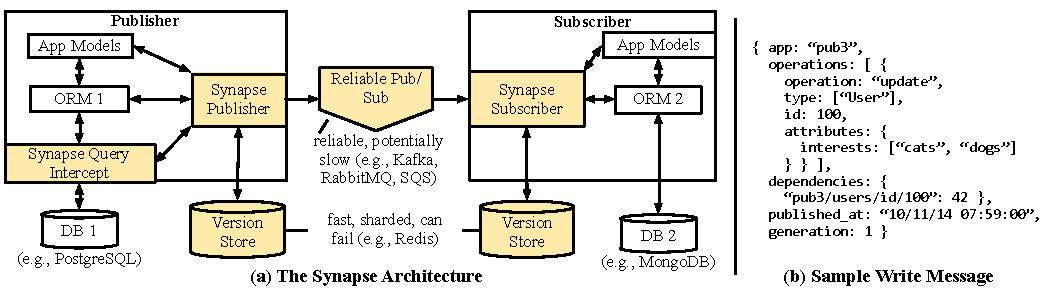
\includegraphics[width=.9\linewidth]{figures/synapse/architecture-less-detail.pdf} \vspace{-12pt}
 \caption{\small {{\bf The \synapse Architecture.}
   (a) \synapse components are shaded.  To replicate data between
       heterogeneous DBs, \synapse marshals the publisher's objects and
       sends them to subscribers, which unmarshal and save them into their
       DBs.  (b) Published message format (JSON).}}
 \label{synapse:fig:architecture}
 \vspace{-15pt}
\end{figure*}

\begin{figure}[t]
\begin{tabular}{c}
\begin{minipage}{.19\textwidth}
\vspace{-7pt}
\begin{lstlisting}[xleftmargin=1pt,framexleftmargin=1pt]
# Publisher 3 (Pub3).
# Runs on MongoDB.
class User
 include Mongoid::Document
 `\specialKeyword{publish}` do
  field :interests
 end
end
\end{lstlisting}
\end{minipage}\vspace{-8pt}\\
\begin{minipage}{.19\textwidth}
\begin{lstlisting}[xleftmargin=1pt,framexleftmargin=1pt]
# Subscriber 3a (Sub3a).
# Runs on any SQL DB.
# Searching for users based on
# interest is not supported.
class User<ActiveRecord::Base
 `\specialKeyword{subscribe}`, :from => :Pub3 do
  field :interests
 end
 serialize :interests
end
\end{lstlisting}
\end{minipage}\vspace{-8pt}\hfill
\end{tabular}
\begin{tabular}{c}
\begin{minipage}{.24\textwidth}
\begin{lstlisting}[xleftmargin=1pt,framexleftmargin=1pt]
# Subscriber 3b (Sub3b).
# Runs on any SQL DB.
# Supports searching for users by interest.
class User < ActiveRecord::Base
 has_many :interests
 `\specialKeyword{subscribe}` :from => :Pub3 do
  field :interests, :as => :interests_virt
 end
 def interests_virt=(tags)
  Interest.add_or_remove(self, tags)
 end
end
class Interest < ActiveRecord::Base
 belongs_to :user
 field :tag
 def self.add_or_remove(user, tags)
   # create/remove interests from DB.
 end
end
\end{lstlisting}
\end{minipage}
\end{tabular}
\vspace{-6pt}
\caption{{\bf Example 3: MongoDB/SQL.}
Shows one publisher running on MongoDB (Pub3) and two SQL subscribers
(Sub3a,b).  Default translations work, but may be suboptimal due to
mismatches between DBs.  Optimizing translation is easy with \synapse.
}
\label{synapse:fig:mongo-sql}
\vspace{-6pt}
\end{figure}

\heading{Example 3: Matching Data Types with Virtual Attributes.}
At times, DBs mismatch on data types.  As an example, we showcase a specific
case of integration between MongoDB and SQL.
MongoDB, a document-oriented database, has become popular among startups
lately thanks to its schemaless data model that allows for frequent
structural changes.  Since the DB imposes so little structure, importing data
into or exporting data from MongoDB is typically similar to
\label{synapse:fig:mongo-to-star}. We choose here a more corner case example to
show \synapse's applicability to complex situations.

\F~\ref{synapse:fig:mongo-sql} shows a MongoDB publisher (Pub3), which leverages a
special MongoDB feature that is not generally available in SQL,
Array types, to store user interests.  \F\ref{synapse:fig:mongo-sql} shows two options
for integrating the interests into a SQL subscriber.  The first option (Sub3a),
which works on all SQL DBs, is to serialize the array field.
In this case, we automatically flatten the array and store it in as text, which would not support efficient queries on interests.

The most straightforward solution to translate this array type to a generic SQL DB is to create an additional model, {\code \footnotesize Interest}, and a one-to-many relationship to it from {\code \footnotesize User}.
Sub3b shows how \synapse's virtual attribute abstraction easily accomplishes
this task, creating the {\code \footnotesize Interest} model and a virtual
attribute  ({\code \footnotesize interests\_virt}) to insert the new interests
received into the separate table.

   comment

   comment
\subsection{\synapse Architecture}
\label{synapse:sec:arch}

\F~\ref{synapse:fig:architecture}(a) shows the \synapse architecture applied to an
application with a single publisher and subscriber. The publisher and subscriber
may be backed by different DBs with distinct engines, data models, or disk
layouts. In our example, the publisher runs on PostgreSQL, a relational DB,
while the subscriber runs on MongoDB, a document DB. At a high level, \synapse
marshals the publisher's model instances (i.e. objects) and publishes them to
subscribers, which unmarshal the objects and persists them through the
subscriber's ORM.

\synapse consists of two DB- and ORM-agnostic modules ({\em \synapse
Publisher} and {\em \synapse Subscriber}), which encapsulate most of the
publishing and subscribing logic, and one DB-specific module ({\em \synapse
Query Intercept}), which intercepts queries and relates them to the objects they
access. On the publisher side, \synapse interposes between the ORMs and the DB
driver to intercept updates of all published models, such as creations, updates,
or deletions of instances -- collectively called {\em writes} -- before they are
committed to the DB. The interposition layer identifies exactly which objects
are being written and passes them onto the {\em \synapse Publisher},
\synapse's DB-independent core. The Publisher then marshals all published
attributes of any created or updated objects, attaches the IDs of any deleted
objects, and constructs a {\em write message}. \synapse sends the message to a
reliable, persistent, and scalable message broker system, which distributes the
message to the subscribers. All writes within a single transaction are combined
into a single message.

The message broker reliably disseminates the write message across subscribers.
Of the many existing message brokers~\cite{jms,kafka,pubsubhubbub,rabbitmq},
we use RabbitMQ~\cite{rabbitmq} in our implementation, using it to provide a
dedicated queue for each subscriber app. Messages in the queue are processed in
parallel by multiple subscriber workers per application, which can be threads,
processes, or machines.

When a new message is available in the message broker, a \synapse subscriber
worker picks it up and unmarshals all received objects by invoking relevant
constructors and attribute setters (using the language's reflection interface).
The worker then persists the update to the underlying DB. When writing to
models, prescribed callbacks are invoked by the ORM. When transactions are
supported, the message is processed within a transaction.

\subsubsection{Model-Driven Replication}
\label{synapse:sec:arch:cross-db-propagation}

To synchronize distinct DBs, \synapse needs to (1) identify the objects being
written on the publisher, (2) marshal them for shipping to the subscribers, (3)
unmarshal back to objects on the subscriber side, (4) and persist them.
Although steps 1 and 4 are DB specific, we leverage ORMs to abstract the DB
specific logic.

To intercept writes, \synapse contains a DB-engine specific query interceptor.
Collecting information about objects written is
generally straightforward, as many DBs can easily output the rows affected
by each query. For example, in SQL, an {\code INSERT}, or {\code DELETE}
query ending with {\code RETURNING *} will return the contents of the
written rows. Many DBs support this feature, including: Oracle, PostgreSQL, SQL
Server, MongoDB, TokuMX, and RethinkDB. For DBs without this feature
(e.g., MySQL, Cassandra), we develop a protocol that involves performing an additional
query to identify data being written; it is safe but somewhat more expensive.

After intercepting a write, \synapse uses the ORM to map from the raw data
written back to application objects (e.g. an instance of the {\tt User} model).
The published attributes of these written object(s) are marshaled to JSON, and published
along with object dependencies (described in
\S\ref{synapse:sec:arch:cross-db-causality}) and a generation number (for recovery,
described in \S\ref{synapse:sec:arch:bootstrapping}). When marshaling objects,
\synapse also includes each object's complete inheritance tree, allowing
subscribers to consume polymorphic models.
\F~\ref{synapse:fig:architecture}(b) shows a write message produced
upon a {\code Post} creation; the post object's marshalling is in the message's
{\code attributes} field.

On the subscriber, \synapse unmarshals a new or updated object by (1)
instantiating a new instance of that type, or finding it in the DB based on its primary key with
the ORM's {\tt find} method, (2) recursively assigning its
subscribed attributes from those included in the message by calling the
object setter methods, and (3) calling the {\code save} or {\code
destroy} method on the object. For a delete operation, step (2) is skipped.
Different ORMs may have different names for these methods (e.g. {\tt find} vs
{\tt find\_by}) but their translation is trivial. Any callbacks specified by the
programmer are automatically called by the ORM.

\subsubsection{Enforcing Delivery Semantics} \label{synapse:sec:arch:cross-db-causality}

\synapse enforces update-message ordering with three different
delivery modes: global, causal, and weak. The performance of each delivery mode
varies, as \S\ref{synapse:sec:evaluation:delivery} will show.

\headingi{Global Ordering:}
The global ordering has the strongest delivery semantics: all publisher writes are serialized via a global lock and delivered to subscribers in order.

\headingi{Causal Ordering:}
Causal ordering identifies, for each write $W$, the prior writes that must
be applied before $W$ to avoid negative effects, such as sending a notification
for a new post to an out-of-date friends set.
\synapse implements causality in a manner very similar to other
causal systems~\cite{ahamad1995causal,Birman:1991:LCA:128738.128742,eiger,bolton}
and its dependency tracking mechanism is described in \S\ref{synapse:sec:arch:deps}.
When a publisher writes in its DB, \synapse updates causal dependency versions in its
version store and then sends the new write to the subscribers, which buffer it.
Each subscriber applies this buffered write to its DB once it has applied all
of the write's dependencies and updates its version store.
In practice, message loss may happen (see \S\ref{synapse:sec:eval:ease-of-use}), which
results in unavailable subscribers.

\headingi{Weak Ordering:}
To maintain availability despite message loss, we provide a weak
ordering mode that never blocks and offers this guarantee: as writes and
updates arrive for a document, they are always increasing.
Since \synapse transmits all published attributes (as opposed to deltas), the subscriber can always fast forward to the latest received version.

   comment

\subsubsection{Tracking Causal Dependencies} \label{synapse:sec:arch:deps}

To enforce causal ordering, \synapse tracks dependencies between updates.  To
first order, \synapse takes an explicit approach to identifying
dependencies, an approach that was adopted by other prior
systems~\cite{bolton,cops,Bailis:2012:PDC:2391229.2391251}.
Specifically, using two constructs in
our API, {\code with\_write\_dep} and {\code with\_read\_dep}, a developer
can specify write and read dependencies, respectively.  Each call takes as a
parameter a URI describing the dependency target. E.g.,
{\code"social\_app/ users/name/"+my\_name\_var} would reference a dependency in
the app {\code SocialApp}, on all instances of the model {\code User} that have
a {\code name} attribute equal to the app's variable, {\code my\_name\_var}.

Unlike prior work using explicit dependencies, \synapse additionally embeds
mechanisms to automatically identify dependencies.  They work well in
practice, but they may not be complete.  \synapse tracks dependencies
within the scope of individual controllers by intercepting read and write
queries and declaring a dependency from any write on all previously read objects
in the cope of that controller execution.  Similarly, all write queries
become dependent on all write queries previously executed in the scope of the
same executing controller. Between controller executions, \synapse tracks
dependencies within the scope of the user session, by including the current user
object as a dependency on all writes.  Finally, \synapse tracks dependencies
within background jobs, e.g., with Sidekiq~\cite{sidekiq}.

In many cases, \synapse can easily determine exactly which objects are read
or written by each query. \synapse automatically intercepts queries of the
form { \code SELECT x,y FROM z WHERE $<$flat expression$>$} with {\code x$=$id}
or when {\em flat expression} specifies a primary key equality constraint.
In our experience, these constitute the vast majority of true dependency
queries.  \synapse detects during testing when a read query does not match its
simple parsing structure and signals these queries to developers, who can
manually provide dependency tracking as necessary.  In the over a dozen
applications we have integrated with \synapse, we have not encountered one
single query that could be considered as a dependency but is not marked as such
by \synapse automatically.  In contrast, prior work relying on explicit
dependencies requires their use with {\em all writes}, which would believe is
onerous for developers and error-prone.

\subsubsection{Bootstrapping and Reliability} \label{synapse:sec:arch:bootstrapping}

When a new subscriber comes online, it must synchronize with the publisher in a
three-step bootstrapping process. First, all current publisher versions are sent
in bulk and saved in the subscriber's version store. Second, all the subscribed model
objects are sent and persisted in the subscriber's DB. Third, all the messages
published during the previous steps are processed to finish synchronizing the
objects and versions. Once all the messages are processed, the subscriber is now
{\em in sync} and operates with the configured delivery semantics.
Subscriber code may call {\code Synapse.bootstrap?} to determine whether \synapse
is still bootstrapping or in sync. \F~\ref{synapse:fig:welcome-email} shows an example of
how the mailer subscriber checks for bootstrapping completion before sending emails.

The subscriber can fail and its queue may grow to an arbitrary size. To
alleviate this issue, \synapse decommissions the subscriber from the
\synapse ecosystem and kills its queue once the queue size reaches a
configurable limit. If the subscriber comes back, \synapse initiates a
{\em partial bootstrap} to get the application back in sync.

Failures may also happen when the version store dies on either the publisher or subscriber
side. When the subscriber's version store dies, a partial bootstrap is initiated. When
the publisher's version store dies, a generation number reliably stored is incremented
and publishing resumes. Messages embed this generation number as shown on
\F~\ref{synapse:fig:architecture}(b). When subscribers see this new generation number
 in messages, they wait until all the previous generation messages are
processed. This generation change incurs a global synchronization barrier and
temporarily slows subscribers.

\subsubsection{Testing Framework}
\label{synapse:sec:testing}

\synapse provides a solid testing framework to help with development and
maintenance of apps.  For instance, \synapse statically checks that subscribers
don't attempt to subscribe to models and attributes that are unpublished,
providing warnings immediately. \synapse also simplifies integration testing by
reusing model factories from publishers on subscribers.  If a publisher
contains a model factory (e.g. data samples), then \synapse will seamlessly
generate integration tests by using these factories to emulate the payloads that
would be received in the subscriber app in a production environment.  This way,
developers are confident that the integration of their ecosystem of applications
is well tested before deploying into the production environment.

\setlength{\tabcolsep}{3pt}
\begin{table}[t]
 \centering {\footnotesize
  \begin{tabular}{l l l l r r}\toprule
   {\bf DB}       & {\bf ORM}    & {\bf Pub?} & {\bf Sub?} & {\bf ORM LoC} &
{\bf DB LoC} \\ \midrule
    PostgreSQL    & ActiveRecord & Y          & Y          & 474           & 44
         \\
    MySQL         & ActiveRecord & Y          & Y          & ''            & 52
         \\
    Oracle        & ActiveRecord & Y          & Y          & ''            & 47
         \\
    MongoDB       & Mongoid      & Y          & Y          & 399           & 0
         \\
    TokuMX        & Mongoid      & Y          & Y          & ''            & 0
         \\
    Cassandra      & Cequel       & Y         & Y          & 219           & 0
         \\
    Elasticsearch & Stretcher    & N/A        & Y          & 0             & 0
         \\
    Neo4j         & Neo4j        & N          & Y          & 0             & 0
         \\
    RethinkDB     & NoBrainer    & N          & Y          & 0             & 0
         \\
    Ephemerals    & N/A           & Y         & N/A          & N/A           & N/A
	\\
    Observers    & N/A           & N/A        & Y          & N/A           & N/A
         \\
  \bottomrule
  \end{tabular}
 }
 \vspace{-0.3cm}
 \caption{{\small {\bf Support for Various DBs.}
 Shows ORM- and DB-specific lines of code (LoC) to support varied DBs.
 For ORMs supporting many DBs (e.g., ActiveRecord), adding a new DB comes for free.}}
 \label{synapse:tab:db-heterogeneity}
\end{table}
\setlength{\tabcolsep}{5pt}

\subsubsection{Supporting New DBs and ORMs}
Adding subscriber support for a new ORM is trivial: a developer need only map the CRUD operations (create/read/update/delete) into \synapse's engine.
To add publisher support for a new ORM, a developer needs to first plug into the ORM's interfaces to intercept queries on their way to the DB (all queries for causality and writes for replication).
Then, the developer needs to add two phase commit hooks to the DB driver for transactional DBs (as discussed in \S\ref{synapse:sec:arch:bootstrapping}).

To illustrate the effort of supporting new DBs and ORMs, we report our development experience on the nine DBs listed in Table~\ref{synapse:tab:db-heterogeneity}.
Our first supported DB was PostgreSQL, taking a single developer approximately one week, and resulting in 474 lines of code specific to ActiveRecord (the ORM; for query intercept) and 44 lines specific to PostgreSQL (for two phase commit). 
After building support for this DB, supporting other SQL DBs, such as MySQL and Oracle, was trivial: about 50 lines of DB-specific, implemented in about a couple of hours for each.
Supporting subsequent DBs (e.g., MongoDB, TokuMX, and Cassandra) was equally simple and took just a few days and 200-300 lines of code per ORM.
Thus, in our experience, supporting various DBs is a very reasonable task for an experienced programmer.
\subsection{Applications}
\label{synapse:sec:apps}

We and others have built or modified 14 web applications to share data with
one another through \synapse.  Those built by others have been
deployed in production by a startup, \crowdtap.  The applications we built
extend popular open-source apps to integrate them into data-driven ecosystems. 
Overall, our development and deployment experience has been positive: we made
{\em no logical changes} to application code, only adding on
average a single line of configuration per attribute of each model published.
At the same time, we achieved great benefits from using \synapse.  

\subsubsection{\synapse at \crowdtap}
\label{synapse:sec:apps:crowdtap}

\crowdtap is an online marketing-services company contracted by major brands such as Verizon, AT\&T, Sony and MasterCard.
\crowdtap has grown rapidly since its founding, and by October 2014 has seen over 450,000 users.
As \crowdtap grew and gained more clients, both their application offering and development team evolved.

At first, engineers attempted to enhance their core application by building new features directly into the same codebase and DB.
However, as new features were added, the data was used in different ways, requiring different indexes and denormalization, bloating the DB.
When features were canceled, traces of their schema changes were often left orphaned.
Moreover, it was difficult to bring newly hired engineers up to speed with the complex and rapidly developing codebase and DB.
To alleviate this issue, engineers factored out some features and provided them
data access via synchronous APIs, but found that this technique was difficult to
get right.
Specifically, a bug in an e-commerce service, which accessed user data from
\crowdtap's core app via a synchronous API, was able to bring down the entire app due to
the lack of performance isolation.  Installing rate limits between the components
of their app was not good option for \crowdtap, and they preferred the
de-coupling that a replication-based solution cross-service would provide.
Synchronization of these DBs then became a challenge.

To address these challenges, \crowdtap began to experiment with \synapse,
first to provide synchronization between their original core app and a separate
targeting service.  These services had previously communicated over a
synchronous API; this API was factored out, and replaced with \synapse,
reducing the app from 1500 LoC to 500 LoC.  While previous attempts to integrate
this feature required the deep knowledge of the core application held by senior
engineers, this integration was performed by a newly-hired engineer.

After this initial integration, two other \crowdtap engineers extracted two other business features, the mailer and the analytics engine from the main application, instead using \synapse to provide data replication.
The email service notifies users of new actions and subscribes to 24 of the core service's models to isolate all notification related aspects within their application, while the analytics engine subscribes to a similarly complex number of models.

\crowdtap's engineering management was so pleased with the ease of development, ease of maintenance, and performance of \synapse, that after this experience, all major features have been built with it (totaling nine apps now).
\F~\ref{synapse:fig:crowdtap-ecosystem} shows the high-level architecture of the \synapse ecosystem at \crowdtap.
\synapse-related code is trivial in size and logic.
The \crowdtap main application consists of approximately 17,000 lines of ruby code, and publishes 257 attributes of 53 different models.
However, the \synapse-related configuration lines are minimal: only 360 (less
than 7 lines of configuration per model, on average).

\crowdtap has chosen different delivery semantics for their various subscribers
(shown with different arrows in \F\ref{synapse:fig:crowdtap-ecosystem}). While all
publishers are configured to support causal delivery mode, subscribers are
configured with either causal or weak delivery modes, depending on their
semantics requirements. The mailer service registers for data from
the Main app in causal mode so as to avoid sending inconsistent emails.
In contrast, the analytics engine lacks stringent order
requirements, hence it selects  a weak consistency model.

\begin{figure}[t]
\centering
   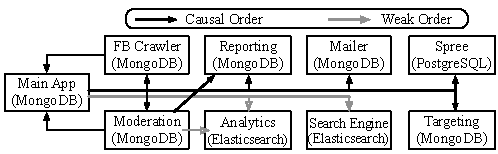
\includegraphics[width=3.3in]{figures/synapse/eco-crowdtap.pdf}
      \vspace{-20pt}
   \caption{\textbf{\crowdtap's services.} Arrows show \synapse connections.}
   \label{synapse:fig:crowdtap-ecosystem}
\end{figure}

\iffalse
\begin{figure}
\begin{minipage}{.225\textwidth}
\begin{lstlisting}[xleftmargin=3pt]
#Semantic Analyzer App (Postgres).
class User < ActiveRecord::Base
 include Synapse::Subscriber
 subscribe :email, from: 'diaspora'
 include Synapse::Publisher
 publish :interests
end
class Post < ActiveRecord::Base
 include Synapse::Subscriber
 subscribe :author_id, :public,
      :contents, from: 'diaspora'
 before_create do  #do the analysis
  #concepts attr defined in schema.
  self.concepts = Textalytics.
           analyze(contents)
 end
 after_create do  #update author
  author.interests += self.concepts
  author.save()
 end
end
\end{lstlisting}
\end{minipage}\hfill
\begin{minipage}{.225\textwidth}
\begin{lstlisting}
#Modified Spree App (MySQL).
class User < ActiveRecord::Base
 include Synapse::Subscriber
 #Subscribe to both the original
 #model and its decoration.
 subscribe :email, from: 'diaspora'
 subscribe :interests,
       from: 'diaspora_topic'
end
# Search controller.
class TargetedSearch<Spree::Search
 def get_base_scope
  tags = current_user.interests
  base_scope = super
  if tags.present?
   base_scope.reorder!('tags.count')
  end
  return base_scope
 end
end
`\ `
\end{lstlisting}
\end{minipage}
\vspace{-0.5cm}
\caption{\small {\bf Targeted Product Search for Spree.}
On the left, the Semantic Analyzer service subscribes to Diaspora and decorates
the {\code User} model with the topics of his latest posts. On the right, a
modified Spree registers for the semantic analyzer's interests decoration, and
returns products related to interests.
}
\label{synapse:fig:spree-code}
\end{figure}
\fi
\begin{figure*}[t]
 \centering \subfigure[{\bf Execution Sample:}
 \ding{172} a user posts on Diaspora. The mailer \ding{173} and semantic
 analyzer \ding{174} receive the post in parallel. Diaspora \ding{175} and Spree
 \ding{176} each receive the decorated model with in parallel.
]{ 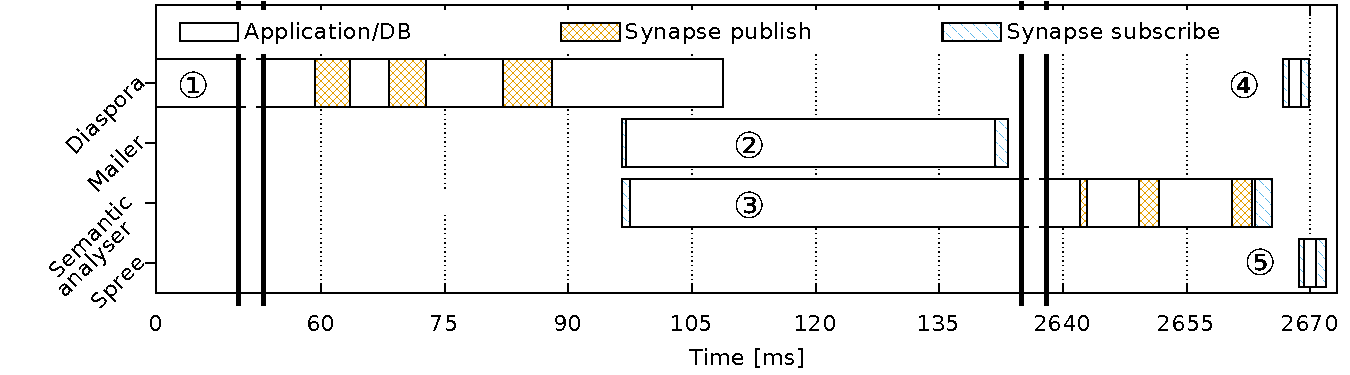
\includegraphics[width=0.48\linewidth]{figures/synapse/diaspora1.pdf}
  \label{synapse:fig:diaspora1}
 } \hfill \subfigure[{\bf Execution with Subscriber Disconnection:}
 \ding{172} and \ding{174} User 1 posts. \ding{173} and \ding{175} User 2 posts.
 Mailer comes online and processes the each users first request \ding{176}, then
 each user's second request \ding{177} in parallel.]{
   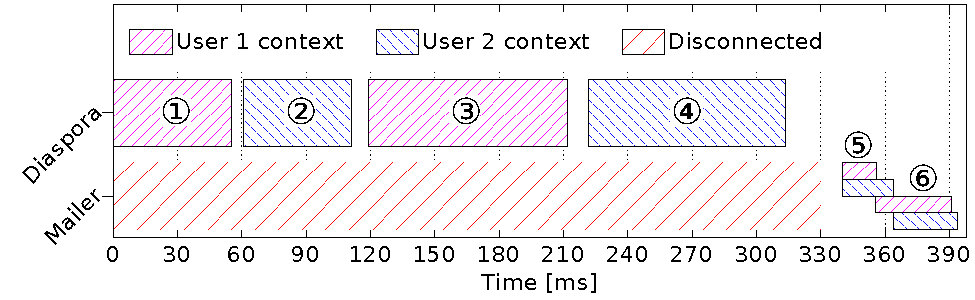
\includegraphics[width=0.48\linewidth]{figures/synapse/diaspora2.pdf}
  \label{synapse:fig:diaspora2}
 }
\vspace{-0.3cm}
 \caption{\small {\bf Execution Samples in Social Ecosystem.}
  Time grows from left to right on x axis.
  (a) Execution in the open-source ecosystem when a user posts a new message.
  (b) Execution when two users post messages with the mailer disconnected.
     }
     \vspace{-0.5cm}
\end{figure*}

\subsubsection{\synapse in Open-Source Apps}
\label{synapse:sec:apps:social}
\begingroup
\setlength{\columnsep}{6pt}
We used \synapse to build a new feature for \emph{Spree}, a popular open source
e-commerce application that powers over
\begin{wrapfigure}{r}{1.4in}
\centering
   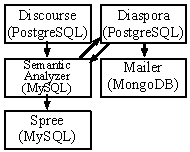
\includegraphics[width=1.2in]{figures/synapse/eco-social.pdf}
      \vspace{-6pt}
   \caption{\textbf{Social Product Recommender.} Arrows show \synapse
connections.}
   \label{synapse:fig:social-ecosystem}
\end{wrapfigure}
45,000 e-commerce websites world
wide~\cite{spree-site}.
By integrating \emph{Diaspora}, a Facebook-like open source social networking
application and \emph{Discourse}, an open source discussion board, with Spree,
we
were able to create a social-based product recommender.
\F\ref{synapse:fig:social-ecosystem} shows the architecture of the ecosystem.
We started by configuring Diaspora and Discourse to publish the models
for posts, friends, and access control lists.
We needed to add only several lines of declarative configuration each app: 23
for Diaspora (compared to its 30K lines of code), 5 for Discourse (compared to
its 21K lines), and 7 for Spree (compared to its 37K lines).

Next, we built a semantic analyzer that subscribes to these posts and extracts topics of interest, decorating Users with apparent topics of interest (using an out-of-the-box semantic analyzer, Textalytics~\cite{textalytics}).
The analyzer publishes its decorated {\code User} model (with user interests) to Spree.
\endgroup

Finally, since Spree did not have \emph{any} recommendation mechanism in place, we added several lines of code to it to implement generic targeted searching.
With this code in place, one can construct as complex a recommendation engine as
one can muster, although our prototype uses a very simple keyword-based matching
between the users' interests and product descriptions. Such code need not be
concerned with where the user's interests come from as they
automatically exist as part of the data model (thanks to \synapse).

\label{synapse:sec:examples}

\synapse addresses many of the challenges of heterogeneous-DB applications automatically through its use of ORMs, often being entirely plug-and-play.
In other cases, the programmer may need to perform explicit translations on the subscriber to align the data models.
Our experience suggests that \synapse's abstractions facilitate these translations, and we illustrate our experience using examples showcasing \synapse's usability with each major class of DB: SQL, document, analytic, and graph.

\begin{figure}[t]
\begin{tabular}{c}
\begin{minipage}{.22\textwidth}
\begin{lstlisting}[xleftmargin=1pt,framexleftmargin=1pt]
# Publisher 1 (Pub1).
# Runs on MongoDB.
class User
 include Mongoid::Document
 `\specialKeyword{publish}` do
  field :name
 end
end
\end{lstlisting}
\end{minipage}\vspace{-8pt}\\
\begin{minipage}{.22\textwidth}
\begin{lstlisting}[xleftmargin=1pt,framexleftmargin=1pt]
# Subscriber 1a (Sub1a).
# Runs on any SQL DB.
class User<ActiveRecord::Base
 `\specialKeyword{subscribe}` :from => :Pub1 do
  field :name
 end
end
\end{lstlisting}
\end{minipage}
\end{tabular}\hfill
\begin{tabular}{c}
\begin{minipage}{0.22\textwidth}
\begin{lstlisting}[xleftmargin=1pt,framexleftmargin=1pt]
# Subscriber 1b (Sub1b).
# Runs on Elasticsearch.
class User < Stretcher::Model
 `\specialKeyword{subscribe}` :from => :Pub1 do
  property :name,:analyzer=>:simple
 end
end
\end{lstlisting}
\end{minipage}\vspace{-8pt}\\
\begin{minipage}{0.22\textwidth}
\begin{lstlisting}[xleftmargin=1pt,framexleftmargin=1pt]
# Subscriber 1c (Sub1c).
# Runs on MongoDB.
class User
 include Mongoid::Document
 `\specialKeyword{subscribe}` :from => :Pub1 do
  field :name
 end
end
\end{lstlisting}
\end{minipage}
\end{tabular}
\vspace{-16pt}
\caption{{\bf Example 1: Basic Integration.}
Shows publishing/subscribing examples with actual ORMs.
\synapse code is trivial.  This is the common case in practice.
}
\label{synapse:fig:mongo-to-star}
\end{figure}

\heading{Example 1: Basic Integrations.}  Our experience suggests that most
integrations with \synapse are entirely automatic and require only simple
annotations of what should be published or subscribed, similar to the ones shown
in \F\ref{synapse:fig:pub-sub}.  To showcase, \F\ref{synapse:fig:mongo-to-star} shows the
integration of a MongoDB publisher (Pub1) with three
subscribers: SQL (Sub1a), Elasticsearch (Sub1b), and
MongoDB (Sub1c). The programmers write their models using
the specific syntax that the underlying ORM
provides.  Barring the {\code {\footnotesize publish/subscribe}} keywords, the
models are exactly how each programmer would model them if they were not using
\synapse (i.e., the data were local to their service).  In our experience
building and deploying \synapse, this is by far the most
frequent case of integration.

That said, there are at times more complex situations, where programmers must
intervene to address mismatches between schemas, supported data types, or
optimal layouts.  We find that even in these cases, \synapse provides just the
right abstractions to help the programmer address them easily and elegantly.
We describe next complex examples, which illustrate \synapse's flexibility
and great added value.  We stress that not all integrations between a given DB
pair will face such difficulties, and vice versa, the same difficulty might be
faced between other pairs than those we illustrate.

\begin{figure}
\begin{tabular}{c}
\begin{minipage}{.23\textwidth}
\begin{lstlisting}[xleftmargin=3pt]
# Publisher 2 (Pub2).
# Runs on any SQL DB.
class User<ActiveRecord::Base
 `\specialKeyword{publish}` do
  field :name
  field :likes
 end
 has_many :friendships
end
class Friendship<ActiveRecord::Base
 `\specialKeyword{publish}` do
  belongs_to :user1, :class => User
  belongs_to :user2, :class => User
 end
end
\end{lstlisting}
\end{minipage}\\
\begin{minipage}{.21\textwidth}
\vspace{0.2cm}
\caption{{\bf Example 2: SQL/Neo4j.}
Pub2 (SQL) stores friendships in their own table; Sub2 (Neo4j) stores
them as edges between Users. }
\vspace{-0.2cm}
\label{synapse:fig:sql-to-neo4j}
\end{minipage}
\end{tabular}\hfill
\begin{tabular}{c}
\begin{minipage}{.21\textwidth}
\begin{lstlisting}
# Subscriber 2 (Sub2).
# Runs on Neo4j.
class User  # persisted model
  include Neo4j::ActiveNode
  `\specialKeyword{subscribe}` :from => :Pub2 do
   property :name
   property :likes
  end
  has_many :both, :friends,
   :class => User
end
class Friendship  # not persisted
 include `\specialKeyword{Synapse::Observer}`
 `\specialKeyword{subscribe}` :from => :Pub2 do
  belongs_to :user1, :class => User
  belongs_to :user2, :class => User
 end
 after_create do
  user1.friends << user2
 end
 after_destroy do
  user1.friends.delete(user2)
 end
end
\end{lstlisting}
\end{minipage}
\end{tabular}
\end{figure}

\heading{Example 2: Mapping Data Models with Observers.}
Different DBs model data in different ways so as to optimize different modes of
accessing it. This example shows how to map the data models between a SQL and
Neo4j DB to best leverage the DBs' functions.  Neo4j, a graph-oriented DB, is
optimized for graph-structured data and queries. It stores relationships between
data items -- such as users in a social network or products in an e-commerce app
-- as edges in a graph and is optimized for queries that must traverse the graph
such as those of recommendation engines. In contrast, SQL stores relationships
in separate tables. When integrating these two DBs, model mismatches may occur.
\F\ref{synapse:fig:sql-to-neo4j} illustrates this use case with an example.

Pub2, the main application, stores Users and their friends in a SQL DB.
Sub2, an add-on recommendation engine, integrates the user and friendship
information into Neo4j to provide users with recommendations of what their
friends or network of friends liked. Its common type of query thus involves
traversing the user's social graph, perhaps several levels deep.  As in the
previous examples, we see here that the programmer defines his subscriber's User
model in the way that he would normally do so for that DB (the top of
Sub2).  However, in this case, \synapse's default translation (achieved by just
annotating data with publish/subscribe) would yield low performance since it
would store both the user and the friendship models as nodes, just like the
publisher's SQL schema does, ignoring the benefits of Neo4j.

To instead store friendships as edges in a graph between users, the programmer
leverages our observer abstraction.  She defines an observer model to
subscribe to the Friendship model, which rather than persisting the data as-is,
simply adds or removes edges among User nodes.  This solution, which involves
minimal and conceptually simple programmer input, lets the subscriber
leverage Neo4j's full power.

\begin{figure*}[t+]
 \centering 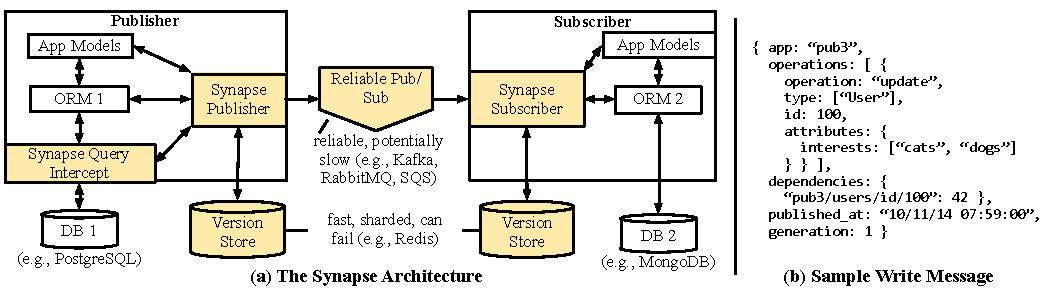
\includegraphics[width=.9\linewidth]{figures/synapse/architecture-less-detail.pdf} \vspace{-12pt}
 \caption{\small {{\bf The \synapse Architecture.}
   (a) \synapse components are shaded.  To replicate data between
       heterogeneous DBs, \synapse marshals the publisher's objects and
       sends them to subscribers, which unmarshal and save them into their
       DBs.  (b) Published message format (JSON).}}
 \label{synapse:fig:architecture}
 \vspace{-15pt}
\end{figure*}

\begin{figure}[t]
\begin{tabular}{c}
\begin{minipage}{.19\textwidth}
\vspace{-7pt}
\begin{lstlisting}[xleftmargin=1pt,framexleftmargin=1pt]
# Publisher 3 (Pub3).
# Runs on MongoDB.
class User
 include Mongoid::Document
 `\specialKeyword{publish}` do
  field :interests
 end
end
\end{lstlisting}
\end{minipage}\vspace{-8pt}\\
\begin{minipage}{.19\textwidth}
\begin{lstlisting}[xleftmargin=1pt,framexleftmargin=1pt]
# Subscriber 3a (Sub3a).
# Runs on any SQL DB.
# Searching for users based on
# interest is not supported.
class User<ActiveRecord::Base
 `\specialKeyword{subscribe}`, :from => :Pub3 do
  field :interests
 end
 serialize :interests
end
\end{lstlisting}
\end{minipage}\vspace{-8pt}\hfill
\end{tabular}
\begin{tabular}{c}
\begin{minipage}{.24\textwidth}
\begin{lstlisting}[xleftmargin=1pt,framexleftmargin=1pt]
# Subscriber 3b (Sub3b).
# Runs on any SQL DB.
# Supports searching for users by interest.
class User < ActiveRecord::Base
 has_many :interests
 `\specialKeyword{subscribe}` :from => :Pub3 do
  field :interests, :as => :interests_virt
 end
 def interests_virt=(tags)
  Interest.add_or_remove(self, tags)
 end
end
class Interest < ActiveRecord::Base
 belongs_to :user
 field :tag
 def self.add_or_remove(user, tags)
   # create/remove interests from DB.
 end
end
\end{lstlisting}
\end{minipage}
\end{tabular}
\vspace{-6pt}
\caption{{\bf Example 3: MongoDB/SQL.}
Shows one publisher running on MongoDB (Pub3) and two SQL subscribers
(Sub3a,b).  Default translations work, but may be suboptimal due to
mismatches between DBs.  Optimizing translation is easy with \synapse.
}
\label{synapse:fig:mongo-sql}
\vspace{-6pt}
\end{figure}

\heading{Example 3: Matching Data Types with Virtual Attributes.}
At times, DBs mismatch on data types.  As an example, we showcase a specific
case of integration between MongoDB and SQL.
MongoDB, a document-oriented database, has become popular among startups
lately thanks to its schemaless data model that allows for frequent
structural changes.  Since the DB imposes so little structure, importing data
into or exporting data from MongoDB is typically similar to
\label{synapse:fig:mongo-to-star}. We choose here a more corner case example to
show \synapse's applicability to complex situations.

\F~\ref{synapse:fig:mongo-sql} shows a MongoDB publisher (Pub3), which leverages a
special MongoDB feature that is not generally available in SQL,
Array types, to store user interests.  \F\ref{synapse:fig:mongo-sql} shows two options
for integrating the interests into a SQL subscriber.  The first option (Sub3a),
which works on all SQL DBs, is to serialize the array field.
In this case, we automatically flatten the array and store it in as text, which would not support efficient queries on interests.  ORMs, such as

The most straightforward solution to translate this array type to a generic SQL DB is to create an additional model, {\code \footnotesize Interest}, and a one-to-many relationship to it from {\code \footnotesize User}.
Sub3b shows how \synapse's virtual attribute abstraction easily accomplishes
this task, creating the {\code \footnotesize Interest} model and a virtual
attribute  ({\code \footnotesize interests\_virt}) to insert the new interests
received into the separate table.

   comment

   comment

\subsection{Evaluation}
\label{synapse:sec:evaluation}

We leverage both our deployment and the applications we built to answer three
core evaluation questions about \synapse: (Q1) How expensive is it
on the publisher side? (Q2) How well does it scale? (Q3) How do its various
delivery modes compare? and (Q4) How useful is it in practice?

To answer these questions, we ran experiments on Amazon AWS with up to 1,000
c3.large instances (2-core, 4GB) running simultaneously to saturate \synapse.
As workloads, we used a mix of \crowdtap production traffic and microbenchmarks
that stress the system in ways that production workload cannot.  Unless
otherwise noted, our evaluation focuses on the causal delivery mode, which is
the default setting in our prototype.  After providing some sample executions,
we next discuss each evaluation question in turn.

\subsubsection{Sample Executions}
\label{synapse:sec:evaluation:sample-runs}

To build intuition into how \synapse behaves and the kinds of overheads it
brings, we show two sample executions of our open-source ecosystem
applications (see \S\ref{synapse:sec:apps:social}). All applications are configured
with a causal delivery mode, hence the examples reflect this mode's functioning.

Figure~\ref{synapse:fig:diaspora1} shows a timeline of the applications' execution
starting with a user's post to Diaspora and ending with Spree's receipt of the
semantically-enhanced User model. We observe that \synapse delivers messages
shortly after publication (within 5ms), in parallel to both the mailer and
the semantic analyzer.  Figure~\ref{synapse:fig:diaspora2}  illustrates visually
\synapse's causal engine in action. It shows two users posting messages on
different Diaspora profiles app while a Mailer subscriber is deployed to notify
a user's friends whenever the user makes a new post.  Initially, the mailer is
disconnected. When the mailer comes back online, it processes messages from the
two users in parallel, but processes each user's posts in serial order, thereby
enforcing causality.

\setlength{\tabcolsep}{4pt}

\subsubsection{Application Overheads (Q1)}
\label{synapse:sec:evaluation:overhead}

We next evaluate \synapse's publishing overheads in the context of real
applications: \crowdtap and the open-source apps we modified. For \crowdtap, we
instrumented \crowdtap's main Web application to record performance metrics and
recorded accesses to the application over the 24 hour period of April 16th,
2014. In total, we recorded one fifth of the traffic totaling 170,000 accesses
to application controllers. For each controller, we measured the average
number of published messages, the average number of dependencies per message
published, the average execution time of the controller, and the average
\synapse overhead, compared to the raw controller latency. This workload is
realistic, however it is not high enough to bottleneck \synapse. We evaluate
the scalability of \synapse directly in \S\ref{synapse:sec:evaluation:scalability}.

\begin{figure*}[t]
 \subfigure[c][{\bf \synapse Overheads at \crowdtap}]{ \raisebox{2.1cm}
{\footnotesize
     \begin{tabular}{l|r|r|r|r|r} \hline
    {\bf Most Popular} & {\bf \% Calls}  & {\bf Published}                     &
\multicolumn{1}{c|}{{\bf Avg.}} & {\bf Controller} & \multicolumn{1}{c}{{\bf
\synapse}}    \\
     {\bf Controllers} & {\bf (of 170k)} & \multicolumn{1}{c|}{{\bf Messages}} &
{\bf \# Deps}                   & {\bf Time (ms)}  & \multicolumn{1}{c}{{\bf
Overhead (ms)}} \\ \hline

      awards/index  & 17.0\% & 0.00 & 0.00  & 56.5  & 0.01 (0.03\%)  \\
     brands/show    & 16.0\% & 0.03 & 0.06  & 97.0  & 0.61 (0.60\%)  \\
     actions/index  & 15.0\% & 0.67 & 13.31 & 170.0 & 12.00 (7.00\%) \\
     me/show        & 12.0\% & 0.00 & 0.00  & 14.7  & 0.00 (0.00\%)  \\
     actions/update & 11.5\% & 3.46 & 9.79  & 240.0 & 65.00 (27.0\%) \\

       \hline
     \multicolumn{6}{l}{ {\bf Average overhead across all 55 controllers:}
4.40\%, standard deviation=8.80\% }
       \vspace{-45pt}
      \end{tabular}
     }
     \label{synapse:tab:crowdtap-overheads}
    }
    \hspace{1cm}
    \subfigure[c][{\bf \synapse Overheads in Real Applications}]{
     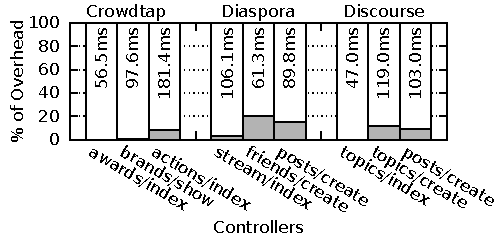
\includegraphics[width=7cm]{figures/synapse/overhead-hist.pdf}
     \label{synapse:fig:app-overheads}
    }
\vspace{-10pt}
    \caption{\small {\bf Application Publishing Overheads.}
      (a) \crowdtap dependencies and overheads, sampled from production data.
          For each of the five most frequently invoked controllers in \crowdtap,
          shows the percent of calls to it, average number of published
          messages, average number of dependencies between messages,
          the average controller execution time, and the average overhead from
          \synapse.
      (b) \synapse overhead (gray parts) for 3 controllers in 3 different
          applications. Labels give the total controller times.
          {\em \synapse publisher overheads are small.}
    }
    \vspace{-15pt}
   \end{figure*}
\setlength{\tabcolsep}{5pt}

   \begin{figure*}[t]
    \centering \subfigure[{\bf Publisher Overhead vs. Dependencies}]{
      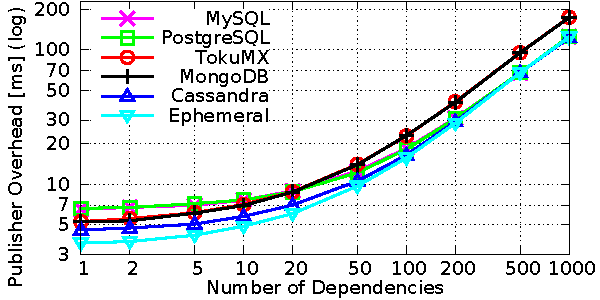
\includegraphics[width=0.31\linewidth]{figures/synapse/overheadvsdeps.pdf}
      \label{synapse:fig:overhead}
    } \hspace{0.1cm} \subfigure[{\bf Throughput on Different DBs}]{
      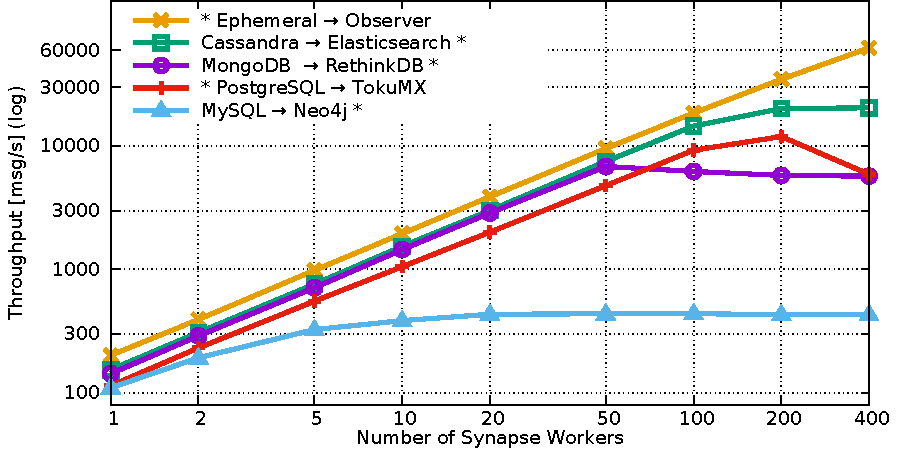
\includegraphics[width=0.31\linewidth]{figures/synapse/db-throughput-vs-workers.pdf}
      \label{synapse:fig:dbs-throughput}
    } \hspace{0.1cm} \subfigure[{\bf Throughput on Various Delivery Semantics}]{
      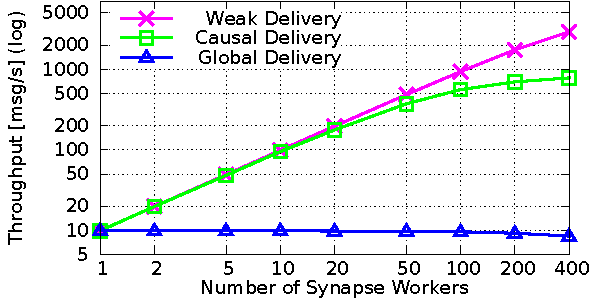
\includegraphics[width=0.31\linewidth]{figures/synapse/throughputvsworkerssaturate.pdf}
      \label{synapse:fig:parallel-throughput}
    }
    \vspace{-0.4cm}
    \caption{\small {\bf Microbenchmark Results.}
     (a) Publisher overhead on different DBs.
     (b) Throughput vs number of workers end to end benchmark.
         Each line represents a different DB setup.
         The slowest end in each pair is annotated with a (*) symbol.
     (c) Throughput vs number of workers with subscribers running a 100ms callback.
         Each line represents a different delivery mode.
         {\em Causal and weak delivery modes scale well.}
     \vspace{-15pt} }
   \end{figure*}

Figure \ref{synapse:tab:crowdtap-overheads} shows our results. In total, 55 controllers
were invoked. We show average overheads across them, as well as detailed
information about the five most frequently accessed controllers, which account
for over 70\% of the traffic. On average, \synapse overheads are low: 4.4\%.
For the most popular two controllers ({\code awards/index} and {\code
brands/show}), the overheads are even lower: 0.03-0.6\%. This is because they
exhibit very few published messages (writes). As expected, \synapse overhead
is higher in controllers that publish more messages, showing a maximum overhead
of 27\% for the controller {\code actions/update}. The number of dependencies also
impacts the overhead, with the controller {\code actions/index} showing a 7\%
overhead for 13.31 dependencies on average per update in that controller.

To complement our \crowdtap results, we measured controllers in our opens-source
applications, as well. Figure \ref{synapse:fig:app-overheads} shows the \synapse
overheads in for several controllers within Diaspora and Discourse (plus
\crowdtap for consistency). Grey areas are \synapse overheads. Overheads
remain low for the two open-source applications. Read-only controllers, such as
{\code stream/index} and {\code topics/index} in Diaspora and Discourse,
respectively, exhibit near-zero overheads; write controllers have up to 20\%
overhead.

These results show that \synapse overheads with real applications are low and
likely unnoticeable to users. However, the results are insufficient to assess
performance under stress, a topic that we discuss next.

\subsubsection{Scalability (Q2)}
\label{synapse:sec:evaluation:scalability}

To evaluate \synapse throughput and latency under high load, we developed a
stress-test microbenchmark, which simulates a social networking site. Users
continuously create posts and comments; comments are related to posts and create
cross-user dependencies. We issue traffic as fast as possible to saturate \synapse, with a
uniform distribution of 25\% posts and 75\% comments. We run this experiment
by deploying identical numbers of publishers and subscribers (up to 400 for
each) in Amazon AWS. As persistence layers, we use several of our supported
DBs and combinations. We applied different DBs as publishers and
subscribers. We measure a variety of metrics, including the overheads for
creating a post, as well as \synapse's throughput.

\heading{Overheads under Heavy Load.}
\F~\ref{synapse:fig:overhead} shows the overheads for different DBs with increasing
numbers of dependencies. Focusing on the one-dependency case (x=1), \synapse
adds overheads ranging from 4.5ms overhead on Cassandra to 6.5ms on PostgreSQL.
This is in comparison to the 0.81ms and 1.9ms latencies that PostgreSQL and
Cassandra, respectively, exhibit {\em without} \synapse. However, compared to
realistic Web controller latencies of tens of ms, these overheads are barely
user-visible. As the number of dependencies increases, the overhead grows slowly
at first, remaining below 10ms for up to 20 dependencies. It then shoots up to a
high 173ms for 1,000 dependencies. Fortunately, as shown in
Figure~\ref{synapse:tab:crowdtap-overheads}, dependencies in real applications remain
fairly low (below 13 on average for \crowdtap).

\heading{Cross-DB Throughputs.}
\F~\ref{synapse:fig:dbs-throughput} shows how \synapse's end-to-end throughput scales
with the number of publisher/subscriber workers, for various DB
combinations, as well as for our
DB-less models (observer to ephemeral). We keep the number of dependencies per
message constant at 4 and shard the version stores on 80 AWS instances. We have not sharded
any of the DBs. For ephemerals, \synapse scales linearly with the number of
workers, reaching a throughput of more than 60,000 msg/s. Even at such high
rates, \synapse does not become a bottleneck.  When DBs are used to
back the publishers and subscribers, the throughput grows linearly with the
number of workers until one of the DBs saturates. Saturation happens when the
slowest of the publisher and subscriber DBs reaches its maximum throughput. The
figure marks with a * the DB that bottlenecks in each combination. For
instance, PostgreSQL bottlenecks at 12,000 writes/s, and Elasticsearch at
20,000 writes/s.

\subsubsection{Delivery Semantic Comparison (Q3)}
\label{synapse:sec:evaluation:delivery}

\synapse supports three delivery modes -- global, causal, and weak -- which
provide different scaling properties.
\F\ref{synapse:fig:parallel-throughput} compares subscriber scalability with 
increased number of subscriber workers available to process writes in parallel.
We configure subscribers with a 100-ms callback delay to simulate
denormalization and DB commits.  The global delivery mode, which requires the
subscriber to commit each write serially, scales poorly.  The causal
delivery mode, which only requires the subscriber to serialize dependent
updates, provides much better scalability.  Its peak throughput is limited by
the inherent parallelism of the workload.  Finally, the weak delivery mode
scales perfectly, never reaching its peak up to 400 subscriber workers.
In practice, we recommend choosing either the causal or weak mode.

\subsubsection{Production Notes (Q4)}
\label{synapse:sec:eval:ease-of-use}

As stated before, \crowdtap has given us very positive feedback on \synapse's
usability and value.  We next relate several interesting stories from
their use of \synapse in production:

\headingi{Supports Live Migrations:} \crowdtap discovered a new use for
\synapse that we had not anticipated.  They used it to implement live DB
migrations.  Unhappy with MongoDB's performance, they migrated their Main App to
TokuMX, another document-oriented DB.  To do so, they bootstrapped a subscriber
app implementing the same functionality as the original app but running on
TokuMX. The subscriber registered for all the Main App's data.  Once it was up
to date, developers just switched their load balancer to the new application and
the migration was completed with little downtime.  They also applied this
mechanism to address otherwise difficult schema migration challenges.

\headingi{Supports Agile Development:} A key aspect in a startup company is
agility.  New features must be rolled out quickly and securely evaluated.
According to \crowdtap, \synapse helps with that. One developer said: ``It
allows us to be very agile. We can experiment with new features, with real
data coming from production.''  For example, during a hackathon, one of the
developers implemented a new reporting prototype. He was able to subscribe to
real time production data without impacting the rest of the system thanks to
\synapse's isolation properties. The business team immediately adopted this
reporting tool, and has been using it ever since.

\headingi{Flexible Semantic Matters:} Interestingly, \crowdtap initially
configured all of its services to run in causal mode.  However, during an
upgrade of RabbitMQ, the (otherwise reliable) message queuing system that
\synapse relies upon, some updates were lost due to an upgrade failure.
Two subscribers deadlocked, and their queues were filling up, since they were
missing dependencies and could not consume the updates.  After timeouts, \synapse's
recovery mechanisms, which rebootstrap the subscribers, kicked in
and the system was unblocked.  However, the subscriber apps were unavailable for
a long period of time. \crowdtap now chooses between causal and weak delivery
modes for each of its subscribers, taking into account its availability/consistency
needs.  It is not an easy choice, but according to them, it {\em can} and {\em must}
be done in a production environment where even reliable components can fail.

\subsubsection{Summary}

We have shown that \synapse is easy to integrate with applications,
and can support multiple, different DBs with reasonable effort. \synapse adds
reasonable overhead on real applications, and is not a bottleneck for
scalability.  Moreover, although still a research prototype, it has been shown
to be valuable beyond its initial promise in production.

\subsection{Related Work}
\label{synapse:sec:related}

\synapse builds upon an immense body of work spanning multiple fields,
including systems, DBs, and software engineering. The major relevant
directions of prior research are: DB replication, data warehousing, federated
DBs, pub/sub systems, and consistency models. We adopt various techniques from
these areas, but instantiate them in unique ways for the domain of modern
MVC-based applications. This lets us break through challenges incurred by more
general prior approaches, and design the first real-time service integration
system that supports both SQL and NoSQL DBs with simple APIs, strong semantics,
and good scalability.

\heading{Same-DB Replication.}
The vast majority of work in DB replication (a good survey of which can be found
in Cecchet, et.al.~\cite{candea-db-replication}) involves replicating data
across different instances of {\em the same DB engine} to increase the DB's
availability, reliability, or throughput.  Traditional DB replication systems
plug in at low levels~\cite{candea-db-replication}, which makes them DB
specific: e.g., they intercept updates inside their engines (e.g., Postgres
replication~\cite{postgres-r}), between the DB driver and the DB engine (e.g.,
MySQL replication~\cite{mysql-replication}), or at the driver level (e.g.,
Middle-R~\cite{middle-r}).  \synapse operates at a much higher level -- the
ORM -- keeping it largely independent of the DB.

\heading{Data Warehousing and Change Capture Systems.}
Data warehousing is a traditional approach for replicating data across
heterogeneous DBs~\cite{books/daglib/0029346,Chaudhuri:1997:ODW:248603.248616}.
While many warehousing techniques~\cite{Chan:1999:DSM:319757.319787,10.1109/TKDE.2005.16,Yang:1997:AMV:645923.673657,dynamo-es-river,mongo-es-river,mosql} are not suitable for
real-time integration, change-data capture systems, one class of data
warehousing systems, are focused on real-time transfer of data updates
between different DB engines. 
Moreover, most traditional data warehousing systems, developed by the DB
community, are focused on replicating data between different SQL DB vendors.
Replication is usually implemented either by installing
triggers that update data in other DBs upon local updates, or by tailing the
transaction log and replaying it on other DBs, as LinkedIn's Databus
does~\cite{databus}.

Triggers are unfortunately not supported by NoSQL DBs, which invalidates this approach for our purposes.
For instance, although the SymmetricDS \cite{symmetricDS} project supports synchronizing data \emph{to} a MongoDB subscriber, it can not replicate data \emph{from} a MongoDB publisher.
Although transaction logs are often supported, it is
generally agreed that parsing these logs is extremely fragile and difficult,
since the logs are proprietary and not guaranteed to be stable across version
updates~\cite{databus}.  \synapse differs from all of these systems by
replicating at the level of ORMs, a much more generic and stable layer, which
lets it replicate data between both SQL and NoSQL engines.

In general, existing systems for replicating between SQL and NoSQL DBs, such as MoSQL \cite{mosql}, MongoRiver \cite{mongo-es-river} and DynamoRiver \cite{dynamo-es-river} work between only specific pairs of DBs, and offer different programming abstractions, semantics and delay properties (most in fact are non-realtime).
In contrast, \synapse provides a novel, unified framework for integrating
many DB types in realtime.

\heading{DB Federation.}
The DB community has long studied the general topic of integrating data from
different DBs into one application, a topic generally known as DB
federation~\cite{ramakrishnan2003database}. Like \synapse, federation systems
establish a translation layer between the different DBs, and typically rely on
DB views -- materialized or not -- to perform translations.  Some systems even
leverage ORMs to achieve uniform access to heterogeneous
DBs~\cite{conf/otm/BalstersH09}. However, these systems are fundamentally
different from \synapse: they let the {\em same} application access data
stored in different DBs uniformly, whereas \synapse lets {\em different}
applications (subscribers) replicate data from one DB (the publisher).  Such
replication, inspired by service-oriented architectures, promotes isolation
and lets the subscribers use the best types of DBs, indexes, and layouts that
are optimal for each case.

Similar to DB federation is projects that aim to create ``universal'' ORMs, which definite a common interface to all DBs (SQL or otherwise), such as Hibernate \cite{hibernate}, DataMapper \cite{datamapper} and CaminteJS \cite{camintejs}.
Such ORMs should in theory ease development of an application that accesses data across different DBs, a problem complementary to that which \synapse solves.
However, since they expose a purely generic interface, such an ORM will encourage a design that does not cater to the individual features provided by each DB.
In contrast, \synapse encourages developers to use different ORMs for different sorts of DBs, providing a common programming abstraction to replicate the data across them.

\heading{Publish/Subscribe Systems.}
\synapse's API is inspired by publish/subscribe systems, a long-time active
area of research~\cite{siena,scribe,thialfi,gryphon,pubsubhubbub,hermes}.
\synapse also incorporates a reliable messaging system,
RabbitMQ~\cite{rabbitmq}, but could use other systems that ensure eventual and
scalable dissemination of messages to subscribers~\cite{kafka,scribe}.
All of these systems require programmers to both specify which messages should
be included in which unit of order, while \synapse contexts {\em
transparently} intercepts data updates, compiles their dependencies
automatically, and publishes them.

\heading{Causality.}
Many consistency models have been developed, which establish varied tradeoffs
between the safety properties of the system (e.g., the accuracy and freshness of
reads) versus its availability and scale~\cite{brewer-conj}.
Among these consistency models, causal
consistency~\cite{Lamport:1978:TCO:359545.359563}
has been demonstrated to provide a good balance between semantics and
scalability~\cite{cops,eiger} and is the strongest model achievable with high
availability under network partitions~\cite{mahajan11cacTR}.  Many
implementations of causal consistency exist in the context of
{\em same-DB replication}~\cite{eiger,cops,bolton,Du:2013:OSC:2523616.2523628,Belaramani:2006:PR:1267680.1267685,Ladin:1992:PHA:138873.138877,bayou,zawirski13swiftcloud,Wang:2013:RSS:2482626.2482661,Birman:1991:LCA:128738.128742}.  \synapse applies these approaches to provide
causal order of update delivery between {\em distinct DBs}.

\subsection{Conclusion} \label{synapse:sec:conclusion}

\synapse is an easy-to-use, strong-semantics cross-DB system for
large-scale, data-driven web service integration. It leverages high-level
abstractions of web application frameworks, Models and Controllers. Models
provided by ORMs are used to equip \synapse of a common translation layer
compatible with many SQL and NoSQL DBs. Controllers are used to
support application-specific consistency semantics.
We have implemented \synapse for Rails
applications, demonstrated that it provides highly scalable performance,
released it open source on GitHub, and deployed it in production
to run the Web services for a company.


\clearpage

% \part{Appendices}
% \appendix
% \chapter{Appendix title}

Sample text sample text sample text. Sample text sample text sample text.
Sample text sample text sample text. Sample text sample text sample text.
Sample text sample text sample text. Sample text sample text sample text.
Sample text sample text sample text. Sample text sample text sample text.
Sample text sample text sample text. Sample text sample text sample text.
Sample text sample text sample text. Sample text sample text sample text.

\section{Sample section}
Sample text sample text sample text. Sample text sample text sample text.
Sample text sample text sample text. Sample text sample text sample text.
Sample text sample text sample text. Sample text sample text sample text.

\subsection{Sample subsection}
Sample text sample text sample text. Sample text sample text sample text.
Sample text sample text sample text. Sample text sample text sample text.
Sample text sample text sample text. Sample text sample text sample text.

\subsection{Sample subsubsection}
Sample text sample text sample text. Sample text sample text sample text.
Sample text sample text sample text. Sample text sample text sample text.
Sample text sample text sample text. Sample text sample text sample text.

\section{Sample section}
Sample text sample text sample text. Sample text sample text sample text.
Sample text sample text sample text. Sample text sample text sample text.
Sample text sample text sample text. Sample text sample text sample text.

\subsection{Sample subsection}
Sample text sample text sample text. Sample text sample text sample text.
Sample text sample text sample text. Sample text sample text sample text.
Sample text sample text sample text. Sample text sample text sample text.


%%%
%%% Bibliography
%%%
\part{Bibliography}
\addcontentsline{toc}{chapter}{Bibliography}
\bibliography{main,refs}
\bibliographystyle{named} 

\end{document}
